\documentclass[a4paper]{article}
\usepackage[ngerman]{babel}
\usepackage[utf8]{inputenc}
\usepackage{multicol}
\usepackage{calc}
\usepackage{ifthen}
\usepackage[landscape]{geometry}
\usepackage{amsmath,amsthm,amsfonts,amssymb}
\usepackage{color,graphicx,overpic}
\usepackage{xcolor, listings}
\usepackage[compact]{titlesec} %less space for headers
\usepackage{mdwlist} %less space for lists
\usepackage{pdflscape}
\usepackage{verbatim}
\usepackage[most]{tcolorbox}
\usepackage[hidelinks,pdfencoding=auto]{hyperref}
\usepackage{bussproofs}
\usepackage{fancyhdr}
\usepackage{lastpage}
\pagestyle{fancy}
\fancyhf{}
\fancyhead[L]{Logik und Logikprogrammierung}
\fancyfoot[L]{\thepage/\pageref{LastPage}}
\renewcommand{\headrulewidth}{0pt} %obere Trennlinie
\renewcommand{\footrulewidth}{0pt} %untere Trennlinie

\pdfinfo{
  /Title (Logik und Logikprogrammierung - Cheatsheet)
  /Creator (TeX)
  /Producer (pdfTeX 1.40.0)
  /Author (Robert Jeutter)
  /Subject ()
}

%%% Code Listings
\definecolor{codegreen}{rgb}{0,0.6,0}
\definecolor{codegray}{rgb}{0.5,0.5,0.5}
\definecolor{codepurple}{rgb}{0.58,0,0.82}
\definecolor{backcolour}{rgb}{0.95,0.95,0.92}
\lstdefinestyle{mystyle}{
 backgroundcolor=\color{backcolour},  
 commentstyle=\color{codegreen},
 keywordstyle=\color{magenta},
 numberstyle=\tiny\color{codegray},
 stringstyle=\color{codepurple},
 basicstyle=\ttfamily,
 breakatwhitespace=false, 
}
\lstset{style=mystyle, upquote=true}

%textmarker style from colorbox doc
\tcbset{textmarker/.style={%
    enhanced,
    parbox=false,boxrule=0mm,boxsep=0mm,arc=0mm,
    outer arc=0mm,left=2mm,right=2mm,top=3pt,bottom=3pt,
    toptitle=1mm,bottomtitle=1mm,oversize}}

% define new colorboxes
\newtcolorbox{hintBox}{textmarker,
  borderline west={6pt}{0pt}{yellow},
  colback=yellow!10!white}
\newtcolorbox{importantBox}{textmarker,
  borderline west={6pt}{0pt}{red},
  colback=red!10!white}
\newtcolorbox{noteBox}{textmarker,
  borderline west={3pt}{0pt}{green},
  colback=green!10!white}

% define commands for easy access
\renewcommand{\note}[2]{\begin{noteBox} \textbf{#1} #2 \end{noteBox}}
\newcommand{\warning}[1]{\begin{hintBox} \textbf{Warning:} #1 \end{hintBox}}
\newcommand{\important}[1]{\begin{importantBox} \textbf{Important:} #1 \end{importantBox}}


% This sets page margins to .5 inch if using letter paper, and to 1cm
% if using A4 paper. (This probably isn't strictly necessary.)
% If using another size paper, use default 1cm margins.
\ifthenelse{\lengthtest { \paperwidth = 11in}}
  { \geometry{top=.5in,left=.5in,right=.5in,bottom=.5in} }
  {\ifthenelse{ \lengthtest{ \paperwidth = 297mm}}
    {\geometry{top=1.3cm,left=1cm,right=1cm,bottom=1.2cm} }
    {\geometry{top=1.3cm,left=1cm,right=1cm,bottom=1.2cm} }
  }

% Redefine section commands to use less space
\makeatletter
\renewcommand{\section}{\@startsection{section}{1}{0mm}%
                {-1ex plus -.5ex minus -.2ex}%
                {0.5ex plus .2ex}%x
                {\normalfont\large\bfseries}}
\renewcommand{\subsection}{\@startsection{subsection}{2}{0mm}%
                {-1explus -.5ex minus -.2ex}%
                {0.5ex plus .2ex}%
                {\normalfont\normalsize\bfseries}}
\renewcommand{\subsubsection}{\@startsection{subsubsection}{3}{0mm}%
                {-1ex plus -.5ex minus -.2ex}%
                {1ex plus .2ex}%
                {\normalfont\small\bfseries}}
\makeatother

% Don't print section numbers
\setcounter{secnumdepth}{0}

\setlength{\parindent}{0pt}
\setlength{\parskip}{0pt plus 0.5ex}  
% compress space
\setlength\abovedisplayskip{0pt}
\setlength{\parskip}{0pt}
\setlength{\parsep}{0pt}
\setlength{\topskip}{0pt}
\setlength{\topsep}{0pt}
\setlength{\partopsep}{0pt}
\linespread{0.5}
\titlespacing{\section}{0pt}{*0}{*0}
\titlespacing{\subsection}{0pt}{*0}{*0}
\titlespacing{\subsubsection}{0pt}{*0}{*0}

\begin{document}

\raggedright
\begin{multicols}{3}\scriptsize
  % multicol parameters
  % These lengths are set only within the two main columns
  %\setlength{\columnseprule}{0.25pt}
  \setlength{\premulticols}{1pt}
  \setlength{\postmulticols}{1pt}
  \setlength{\multicolsep}{1pt}
  \setlength{\columnsep}{2pt}

  \subsubsection{Probleme mit natürlicher Sprache}

  \begin{enumerate*}
    \item Zuordnung von Wahrheitswerten zu natürlichsprachigen Aussagen ist problematisch. (Ich habe nur ein bißchen getrunken.)
    \item Natürliche Sprache ist oft schwer verständlich.
    \item Natürliche Sprache ist mehrdeutig.
    \item Natürliche Sprache hängt von Kontext ab.
  \end{enumerate*}

  \section{Aussagenlogik}
  In der Aussagenlogik gehen wir von ``Aussagen'' aus, denen wir (zumindest prinzipiell) Wahrheitswerte zuordnen können.

  Die Aussagen werden durch ``Operatoren'' verbunden.

  Für zusammengesetzten Aussagen verwenden wir $\varphi,\psi$ usw.

  Durch die Wahl der erlaubten Operatoren erhält man unterschiedliche ``Logiken''.

  Da der Wahrheitswert einer zusammengesetzten Aussage nur vom Wahrheitswert der Teilaussagen abhängen soll, sind Operatoren wie ``weil'' oder ``obwohl'' nicht zulässig.

  \subsection{Syntax der Aussagenlogik}
  Eine atomare Formel hat die Form $p_i$ (wobei $i\in\mathbb{N}=\{0,1,...\}$). Formeln werden durch folgenden induktiven Prozess definiert:
  \begin{enumerate*}
    \item Alle atomaren Formeln und $\bot$ sind Formeln.
    \item Falls $\varphi$ und $\psi$ Formeln sind, sind auch $(\varphi\wedge\psi),(\varphi\wedge\psi)$($\varphi \rightarrow\psi$) und $\lnot\varphi$Formeln.
    \item Nichts ist Formel, was sich nicht mittels der obigen Regeln erzeugen läßt.
  \end{enumerate*}

  Beispielformel: $\lnot((\lnot p_4 \vee p_1)\wedge\bot)$

  Präzedenz der Operatoren:
  \begin{itemize*}
    \item $\leftrightarrow$ bindet am schwächsten
    \item $\rightarrow$\ldots{}
    \item $\vee$\ldots{}
    \item $\wedge$\ldots{}
    \item $\lnot$ bindet am stärksten
  \end{itemize*}

  \subsection{Natürliches Schließen}
  Ein (mathematischer) Beweis zeigt, wie die Behauptung aus den Voraussetzungen folgt.
  Analog zeigt ein ``Beweisbaum'' (=``Herleitung'' = ``Deduktion''), wie eine Formel der Aussagenlogik aus Voraussetzungen (ebenfalls Formeln der Aussagenlogik) folgt.
  Diese ``Deduktionen'' sind Bäume, deren Knoten mit Formeln beschriftet sind:
  \begin{itemize*}
    \item an der Wurzel steht die Behauptung (= Konklusion $\varphi$)
    \item an den Blättern stehen Voraussetzungen (= Hypothesen oder Annahmen aus $\Gamma$)
    \item an den inneren Knoten stehen ``Teilergebnisse'' und ``Begründungen''
  \end{itemize*}

  \subsection{Konstruktion von Deduktionen}
  Aus der Annahme der Aussage $\varphi$ folgt $\varphi$ unmittelbar: eine triviale Deduktion

  $\varphi$ mit Hypothesen $\{\varphi\}$ und Konklusion $\varphi$.

  \subsubsection{Konjunktionseinführung}
  Ist D eine Deduktion von $\varphi$ mit Hypothesen aus $\Gamma$ und ist E eine Deduktion von $\psi$ mit Hypothesen aus $\Gamma$, so ergibt sich die folgende Deduktion von $\varphi\wedge\psi$ mit Hypothesen aus $\Gamma$:
  \begin{prooftree}
    \AxiomC{$\varphi$}
    \AxiomC{$\psi$}
    \RightLabel{\scriptsize ($\wedge I$)}
    \BinaryInfC{$\varphi\wedge\psi$}
  \end{prooftree}

  \subsubsection{Konjunktionselimination}
  Ist D eine Deduktion von $\varphi\wedge\psi$ mit Hypothesen aus $\Gamma$, so ergeben sich die folgenden Deduktionen von $\varphi$ bzw. von $\psi$ mit Hypothesen aus $\Gamma$:

  \begin{prooftree}
    \AxiomC{$\varphi\wedge\psi$}
    \RightLabel{\scriptsize ($\wedge E_1$)}
    \UnaryInfC{$\varphi$}
  \end{prooftree}
  \begin{prooftree}
    \AxiomC{$\varphi\wedge\psi$}
    \RightLabel{\scriptsize ($\wedge E_2$)}
    \UnaryInfC{$\psi$}
  \end{prooftree}

  \subsubsection{Implikationseinführung}
  Ist D eine Deduktion von $\psi$ mit Hypothesen aus $\Gamma\cup\{\varphi\}$, so ergibt sich die folgende Deduktion von $\varphi\rightarrow\psi$ mit Hypothesen aus $\Gamma$:
  \begin{prooftree}
    \AxiomC{$\psi$}
    \RightLabel(\scriptsize ($\rightarrow I)$)
    \UnaryInfC{$\varphi\rightarrow\psi$}
  \end{prooftree}

  \subsubsection{Implikationselimination oder modus ponens}
  Ist D eine Deduktion von $\varphi$ mit Hypothesen aus $\Gamma$ und ist E eine Deduktion von $\varphi\rightarrow\psi$ mit Hypothesen aus $\Gamma$, so ergibt sich die folgende Deduktion von $\psi$ mit Hypothesen aus $\Gamma$:
  \begin{prooftree}
    \AxiomC{$\varphi$}
    \AxiomC{$\varphi\rightarrow\psi$}
    \RightLabel(\scriptsize ($\rightarrow E)$)
    \BinaryInfC{$\varphi$}
  \end{prooftree}

  \subsubsection{Disjunktionselimination}
  Ist D eine Deduktion von $\varphi\vee\psi$ mit Hypothesen aus $\Gamma$, ist E eine Deduktion von $\sigma$ mit Hypothesen aus $\Gamma\cup\{\varphi\}$und ist F eine Deduktion von $\sigma$ mit Hypothesen aus $\Gamma\cup\{\psi\}$, so ergibt sich die folgende Deduktion von $\sigma$ mit Hypothesen aus $\Gamma$:
  \begin{prooftree}
    \AxiomC{$\varphi\vee\psi$}
    \AxiomC{$\sigma$}
    \AxiomC{$\sigma$}
    \RightLabel(\scriptsize ($\vee E)$)
    \TrinaryInfC{$\sigma$}
  \end{prooftree}

  \subsubsection{Negationseinführung}
  Ist D eine Deduktion von $\bot$ mit Hypothesen aus $\Gamma\cup\{\varphi\}$, so ergibt sich die folgende Deduktion von $\lnot\varphi$ mit Hypothesen aus $\Gamma$:
  \begin{prooftree}
    \AxiomC{$\bot$}
    \RightLabel(\scriptsize ($\lnot I)$)
    \UnaryInfC{$\varphi$}
  \end{prooftree}

  \subsection{Negationselimination}
  Ist D eine Deduktion von $\lnot\varphi$ mit Hypothesen aus $\Gamma$ und ist E eine Deduktion von $\varphi$ mit Hypothesen aus $\gamma$, so ergibt sich die folgende Deduktion von $\bot$ mit Hypothesen aus $\Gamma$:
  \begin{prooftree}
    \AxiomC{$\lnot\varphi$}
    \AxiomC{$\varphi$}
    \RightLabel(\scriptsize ($\lnot E)$)
    \BinaryInfC{$\bot$}
  \end{prooftree}

  \subsubsection{Falsum}
  Ist D eine Deduktion von $\bot$ mit Hypothesen aus $\Gamma$, so ergibt sich die folgende Deduktion von $\varphi$ mit Hypothesen aus $\Gamma$:
  \begin{prooftree}
    \AxiomC{$\bot$}
    \RightLabel(\scriptsize ($\bot)$)
    \UnaryInfC{$\varphi$}
  \end{prooftree}

  \subsubsection{reductio ad absurdum}
  Ist D eine Deduktion von $\bot$ mit Hypothesen aus $\Gamma\cup\{\lnot\varphi\}$, so ergibt sich die folgende Deduktion von $\varphi$ mit Hypothesen aus $\Gamma$:
  \begin{prooftree}
    \AxiomC{$\bot$}
    \RightLabel(\scriptsize ($raa)$)
    \UnaryInfC{$\varphi$}
  \end{prooftree}

  \subsection{Regeln des natürlichen Schließens}
  \note{Definition}{Für eine Formelmenge $\Gamma$ und eine Formel $\varphi$ schreiben wir $\Gamma\Vdash\varphi$ wenn es eine Deduktion gibt mit Hypothesen aus $\Gamma$ und Konklusion $\varphi$. Wir sagen "$\varphi$ ist eine syntaktische Folgerung von $\Gamma$".

    Eine Formel $\varphi$ ist ein Theorem, wenn $\varnothing\Vdash\varphi$ gilt.}

  \subsubsection{Bemerkung}
  $\Gamma\Vdash\varphi$ sagt (zunächst) nichts über den Inhalt der Formeln in $\Gamma\cup\{\varphi\}$ aus, sondern nur über die Tatsache, dass $\varphi$ mithilfe des natürlichen Schließens aus den Formeln aus $\Gamma$ hergeleitet werden kann.

  Ebenso sagt "$\varphi$ ist Theorem" nur, dass $\varphi$ abgeleitet werden kann, über "Wahrheit" sagt dieser Begriff (zunächst) nichts aus.

  \subsubsection{Satz}
  Für alle Formeln $\varphi$ und $\psi$ gilt $\{\lnot(\varphi\vee\psi)\}\Vdash\lnot\varphi\wedge\lnot\psi$.

  Beweis: Wir geben eine Deduktion an...
  \begin{itemize*}
    \item $\{\lnot\varphi\wedge\lnot\psi\}\Vdash\lnot(\varphi\vee\psi)$
    %\includegraphics[width=\linewidth]{Assets/Logik-beispiel-1.png)
    \item $\{\lnot\varphi\vee\lnot\psi\}\Vdash\lnot(\varphi\wedge\psi)$
    %\includegraphics[width=\linewidth]{Assets/Logik-beispiel-2.png)
    \item $\{\varphi\vee\psi\} \Vdash \psi\vee\varphi$
    %\includegraphics[width=\linewidth]{Assets/Logik-beispiel-3.png)
  \end{itemize*}

  \subsubsection{Satz}
  Für jede Formel $\varphi$ ist $\lnot\lnot\varphi\rightarrow\varphi$ ein Theorem.

  Beweis: Wir geben eine Deduktion mit Konklusion $\lnot\lnot\varphi\rightarrow\varphi$ ohne Hypothesen an...

  %\includegraphics[width=\linewidth]{Assets/Logik-beispiel-5.png)

  \subsubsection{Satz}
  Für jede Formel $\varphi$ ist $\varphi\vee\lnot\varphi$ ein Theorem.

  Beweis: Wir geben eine Deduktion mit Konklusion $\varphi\vee\lnot\varphi$ ohne Hypothesen an...

  %\includegraphics[width=\linewidth]{Assets/Logik-beispiel-6.png)

  Bemerkung: Man kann beweisen, dass jede Deduktion der letzten beiden Theoreme die Regel (raa) verwendet, sie also nicht "intuitionistisch" gelten.

  \subsubsection{Satz}
  $\{\lnot(\varphi\wedge\psi)\}\Vdash\lnot\varphi\vee\lnot\psi$

  %\includegraphics[width=\linewidth]{Assets/Logik-beispiel-4.png)

  \subsection{Semantik}
  Formeln sollen Verknüpfungen von Aussagen widerspiegeln, wir haben dies zur Motivation der einzelnen Regeln des natürlichen Schließens genutzt.
  Aber die Begriffe "syntaktische Folgerung" und "Theorem" sind rein syntaktisch definiert.

  Erst die jetzt zu definierende "Semantik" gibt den Formeln "Bedeutung".

  Idee der Semantik: wenn man jeder atomaren Formel $p_i$ einen Wahrheitswertzuordnet, so kann man den Wahrheitswert jeder Formel berechnen.

  Es gibt verschiedene Möglichkeiten, Wahrheitswerte zu definieren:
  \begin{itemize*}
    \item zweiwertige oder Boolesche Logik $B=\{0,1\}$: Wahrheitswerte "wahr"=1 und "falsch"= 0
    \item dreiwertige Kleene-Logik $K_3=\{0,\frac{1}{2},1\}$: zusätzlicher Wahrheitswert "unbekannt"$=\frac{1}{2}$
    \item Fuzzy-Logik $F=[0,1]$: Wahrheitswerte sind "Grad der Überzeugtheit"
    \item unendliche Boolesche Algebra $B_R$= Menge der Teilmengen von $\mathbb{R}$; $A\subseteq\mathbb{R}$ ist "Menge der Menschen, die Aussage für wahr halten"
    \item Heyting-Algebra $H_R$= Menge der offenen Teilmengen von $\mathbb{R}$
    \item Erinnerung: $A\subseteq\mathbb{R}$ offen, wenn $\forall a\in A\exists\epsilon >0:(a-\epsilon,a+\epsilon)\subseteq A$, d.h., wenn $A$ abzählbare Vereinigung von offenen Intervallen $(x,y)$ ist.
  \end{itemize*}

  Beispiele:
  \begin{itemize*}
    \item offen: $(0,1), \mathbb{R}_{>0}, \mathbb{R}\backslash\{0\}, \mathbb{R}\backslash\mathbb{N}$
    \item nicht offen: $[1,2), \mathbb{R}_{\geq 0}, \mathbb{Q}, \mathbb{N}, \{\frac{1}{n} | n\in\mathbb{N}\}, \mathbb{R}\backslash\mathbb{Q}$
  \end{itemize*}


  Sei W eine Menge von Wahrheitswerten.\\
  Eine W-Belegung ist eine Abbildung $B:V\rightarrow W$, wobei $V\subseteq\{p_0 ,p_1 ,...\}$ eine Menge atomarer Formeln ist.

  Die W-Belegung $B:V\rightarrow W$ paßt zur Formel $\phi$, falls alle atomaren Formeln aus $\phi$ zu V gehören.

  Sei nun B eine W-Belegung. Was ist der Wahrheitswert der Formel $p_0\vee p_1$ unter der Belegung B?

  Zur Beantwortung dieser Frage benötigen wir eine Funktion $\vee_W :W\times W\rightarrow W$ (analog für $\wedge,\rightarrow,\lnot$).

  \subsection{Wahrheitswertebereiche}
  \note{Definition}{Sei W eine Menge und $R\subseteq W\times W$ eine binäre Relation.
    \begin{itemize*}
      \item R ist reflexiv, wenn $(a,a)\in R$ für alle $a\in W$ gilt.
      \item R ist antisymmetrisch, wenn $(a,b),(b,a)\in R$ impliziert, dass $a=b$ gilt (für alle $a,b\in W$).
      \item R ist transitive, wenn $(a,b),(b,c)\in R$ impliziert, dass $(a,c)\in R$ gilt (für alle $a,b,c\in W$).
      \item R ist eine Ordnungsrelation, wenn R reflexiv, antisymmetrisch und transitiv ist. In diesem Fall heißt das Paar $(W,R)$ eine partiell geordnete Menge.
    \end{itemize*}
  }

  Beispiel
  \begin{enumerate*}
    \item Sei $\leq$ übliche Ordnung auf $\mathbb{R}$und $W\subseteq\mathbb{R}$. Dann ist $(W,\leq)$ partiell geordnete Menge.
    \item Sei $X$ eine Menge und $W\subseteq P(X)$. Dann ist $(W,\subseteq)$ partiell geordnete Menge.
    \item Sei $W=P(\sum *)$ und $\leq_p$ die Relation "es gibt Polynomialzeitreduktion" (vgl. "Automaten, Sprachen und Komplexität"). Diese Relation ist reflexiv, transitiv, aber nicht antisymmetrisch (denn $3-SAT\leq_p HC$ und $HC\leq_p 3-SAT$).
  \end{enumerate*}

  \note{Definition}{Sei $(W,\leq)$ partiell geordnete Menge, $M\subseteq W$ und $a\in W$.
    \begin{itemize*}
      \item a ist obere Schranke von $M$, wenn $m\leq a$ für alle $m\in M$ gilt.
      \item a ist kleinste obere Schranke oder Supremum von $M$, wenn $a$ obere Schranke von $M$ ist und wenn $a\leq b$ für alle oberen Schranken $b$ von $M$ gilt. Wir schreiben in diesem Fall $a=sup \ M$.
      \item a ist untere Schranke von $M$, wenn $a\leq m$ für alle $m\in M$ gilt.
      \item a ist größte untere Schranke oder Infimum von $M$, wenn a untere Schranke von $M$ ist und wenn $b\leq a$ für alle unteren Schranken $b$ von $M$ gilt. Wir schreiben in diesem Fall $a=inf\ M$.
    \end{itemize*}
  }

  Beispiel
  \begin{enumerate*}
    \item  betrachte $(W,\leq)$ mit $W=\mathbb{R}$ und $\leq$ übliche Ordnung auf $\mathbb{R}$.
    \begin{itemize*}
      \item Dann gelten $sup[0,1] = sup(0,1) =1$.
      \item $sup\ W$ existiert nicht (denn $W$ hat keine obere Schranke).
    \end{itemize*}
    \item betrachte $(W,\subseteq)$ mit $X$ Menge und $W =P(X)$.
    \begin{itemize*}
      \item $sup\ M=\bigcup_{A\in M} A$ für alle $M\subseteq W$
    \end{itemize*}
    \item betrachte $(W,\subseteq)$ mit $W=\{\{0\},\{1\},\{0,1,2\},\{0,1,3\}\}$.
    \begin{itemize*}
      \item $sup\{\{0\},\{0,1,2\}\}=\{0,1,2\}$
      \item $\{0,1,2\}$ und $\{0,1,3\}$ sind die oberen Schranken von $M=\{\{0\},\{1\}\}$, aber $M$ hat kein Supremum
    \end{itemize*}
  \end{enumerate*}

  \note{Definition}{ Ein (vollständiger) Verband ist eine partiell geordnete Menge $(W,\leq)$, in der jede Menge $M\subseteq W$ ein Supremum $sup\ M$ und ein Infimum $inf\ M$ hat.}
  In einem Verband $(W,\leq)$ definieren wir:
  \begin{itemize*}
    \item $0_W = inf\ W$ und $1_W= sup\ W$
    \item $a\wedge_W b= inf\{a,b\}$ und $a\vee_W b= sup\{a,b\}$ für $a,b\in W$
  \end{itemize*}

  Bemerkung: In jedem Verband $(W,\leq)$ gelten $0_W= sup\ \varnothing$ und $1_W= inf\ \varnothing$ (denn jedes Element von $W$ ist obere und untere Schranke von $\varnothing$).

  \note{Definition}{Ein Wahrheitswertebereich ist ein Tupel $(W,\leq,\rightarrow W,\lnot W)$, wobei $(W,\leq)$ ein Verband und $\rightarrow W:W^2 \rightarrow W$ und $\lnot W:W\rightarrow W$  Funktionen sind.}

  \subsubsection{Beispiel}
  \begin{itemize*}
    \item Der Boolesche Wahrheitswertebereich B ist definiert durch die Grundmenge $B=\{0,1\}$, die natürliche Ordnung $\leq$ und die Funktionen $\lnot_B (a) = 1-a$, $\rightarrow_B(a,b) = max(b, 1 -a)$. Hier gelten:
    \begin{itemize*}
      \item $0_B=0$, $1_B= 1$,
      \item $a\wedge_B b= min(a,b)$, $a\vee_B b= max(a,b)$
    \end{itemize*}
    \item Der Kleenesche Wahrheitswertebereich $K_3$ ist definiert durch die Grundmenge $K_3=\{0,\frac{1}{2},1\}$ mit der natürlichen Ordnung $\leq$ und durch die Funktionen $\lnot_{K_3} (a) = 1 -a $, $\rightarrow_{K_3} (a,b) = max(b, 1-a)$. Hier gelten:
    \begin{itemize*}
      \item $\lnot_{K_3} = 0$, $1_{K_3} = 1$
      \item $a\wedge_{K_3} b= min(a,b)$, $a\vee_{K_3} b= max(a,b)$
    \end{itemize*}
    \item Der Wahrheitswertebereich F der Fuzzy-Logik ist definiert durch die Grundmenge $F=[0,1]\subseteq\mathbb{R}$ mit der natürlichen Ordnung $\leq$ und durch die Funktionen $\lnot_F (a) = 1-a$, $\rightarrow_F (a,b) = max(b, 1-a)$. Hier gelten:
    \begin{itemize*}
      \item $0_F= 0$, $1_F= 1$
      \item $a\wedge_F b= min(a,b)$, $a\vee_F b= max(a,b)$
    \end{itemize*}
    \item Der Boolesche Wahrheitswertebereich $B_R$ ist definiert durch die Grundmenge $B_R=\{A|A\subseteq \mathbb{R}\}$ mit der Ordnung $\subseteq$ und durch die Funktionen $\lnot_{B_R} (A) =\mathbb{R}\backslash A$, $\rightarrow_{B_R} (A,B) = B\cup\mathbb{R}\backslash A$. Hier gelten:
    \begin{itemize*}
      \item $0_{B_R}=\varnothing$, $1_{B_R}=\mathbb{R}$
      \item $A\wedge_{B_R} B=A\cap B$, $A\vee_{B_R} B=A\cup B$
    \end{itemize*}
    \item Der Heytingsche Wahrheitswertebereich $H_R$ ist definiert durch die Grundmenge $H_{mathbb{R}} =\{A\subseteq\mathbb{R} | \text{A ist offen}\}$, die Ordnung $\subseteq$ und durch die Funktionen $\lnot_{H_R} (A) = Inneres(\mathbb{R}\backslash A)$, $\rightarrow_{H_R} (A,B) =Inneres(B\cup \mathbb{R}\backslash A)$. Hier gelten:
    \begin{itemize*}
      \item $0_{H_R}=\varnothing$, $1_{H_R}=\mathbb{R}$
      \item $A\wedge_{H_R} B= A\cap B$, $A\vee_{H_R} B=A\cup B$
      \item Erinnerung: $Inneres(A) =\{a\in A|\exists \epsilon > 0 : (a-\epsilon,a+\epsilon)\subseteq A\}$
      \item Beispiele: $Inneres((0,1))=(0,1)=Inneres([0,1]),Inneres(N)=\varnothing,Inneres(\mathbb{R}_{\geq 0}) = \mathbb{R}_{> 0}$
    \end{itemize*}
  \end{itemize*}


  Sei W ein Wahrheitswertebereich und B eine W-Belegung. Induktiv über den Formelaufbau definieren wir den Wahrheitswert $\hat{B}(\phi)\in W$ jeder zu $B$ passenden Formel $\phi$:
  \begin{itemize*}
    \item $\hat{B}(\bot) = 0_W$
    \item $\hat{B}(p) = B(p)$ falls $p$ eine atomare Formel ist
    \item $\hat{B}((\phi\wedge \psi )) = \hat{B}(\phi)\wedge_W \hat{B}(\psi )$
    \item $\hat{B}((\phi\vee \psi )) = \hat{B}(\phi)\vee_W \hat{B}(\psi )$
    \item $\hat{B}((\phi\rightarrow \psi )) = \rightarrow W(\hat{B}(\phi),\hat{B}(\psi ))$
    \item $\hat{B}(\lnot\phi) = \lnot W(\hat{B}(\phi))$
  \end{itemize*}

  Wir schreiben im folgenden $B(\phi)$ anstatt $\hat{B}(\phi)$.

  Beispiel: Betrachte die Formel $\phi= ((p\wedge q)\rightarrow (q\wedge p))$.
  \begin{itemize*}
    \item Für eine beliebige B-Belegung $B:\{p,q\}\rightarrow B$ gilt $B((p\wedge q)\rightarrow (q\wedge p)) = max(B(q\wedge p), 1 -B(p\wedge q)) = max(min(B(q),B(p)), 1 -min(B(p),B(q))) = 1 = 1_B$
    \item Für die $K_3$-Belegung $B:\{p,q\}\rightarrow K_3$ mit $B(p) =B(q) = \frac{1}{2}$ gilt $B((p\wedge q)\rightarrow (q\wedge p)) = max(B(q\wedge p), 1 -B(p\wedge q))= max(min(B(q),B(p)), 1 -min(B(p),B(q))) = \frac{1}{2} \not= 1_{K_3}$
    \item analog gibt es eine F-Belegung $B:\{p,q\}\rightarrow F$, so dass $B((p\wedge q)\rightarrow (q\wedge p)) \not = 1_F$ gilt.
    \item Für eine beliebige $H_{mathbb{R}}$-Belegung $B:\{p,q\}\rightarrow H_R$ gilt $B((p\wedge q)\rightarrow (q\wedge p)) = Inneres(B(q\wedge p)\cup \mathbb{R}\backslash B(p\wedge q)) = Inneres((B(q)\cap B(p))\cup \mathbb{R}\backslash (B(p)\cap B(q))) = Inneres(\mathbb{R}) = \mathbb{R} = 1_{H_R}$
  \end{itemize*}

  \subsection{Folgerung und Tautologie}
  Sei W ein Wahrheitswertebereich.
  Eine Formel $\phi$ heißt eine W-Folgerung der Formelmenge $\Gamma$, falls für jede W-Belegung B, die zu allen Formeln aus $\Gamma \cup\{\phi\}$ paßt, gilt:
  $inf\{B(\gamma )|\gamma \in \Gamma \}\leq B(\phi)$

  Wir schreiben $\Gamma \Vdash W\phi$, falls $\phi$ eine W-Folgerung von $\Gamma$ ist.

  Bemerkung: Im Gegensatz zur Beziehung $\Gamma \vdash \phi$, d.h. zur syntaktischen Folgerung, ist $\Gamma \Vdash W \phi$ eine semantische Beziehung.

  Eine W-Tautologie ist eine Formel $\phi$ mit $\varnothing \Vdash W\phi$, d.h. $B(\phi) = 1_W$ für alle passenden W-Belegungen B (denn $inf\{\hat{B}(\gamma )|\gamma \in \varnothing \}= inf \varnothing = 1_W)$.

  Wahrheitstafel für den Booleschen Wahrheitswertebereich B:

  | RL  | AK  | BK  | $AK\vee BK$ | $AK\rightarrow BK$ | $(BK\wedge RL)\rightarrow\lnot AK$ | RL  | $\lnot AK$ |
  | --- | --- | --- | ----------- | ------------------ | ---------------------------------- | --- | ---------- |
  | 0   | 0   | 0   | 0           | 1                  | 1                                  | 0   | 1          |
  | 0   | 0   | 1   | 1           | 1                  | 1                                  | 0   | 1          |
  | 0   | 1   | 0   | 1           | 0                  | 1                                  | 0   | 0          |
  | 0   | 1   | 1   | 1           | 1                  | 1                                  | 0   | 0          |
  | 1   | 0   | 0   | 0           | 1                  | 1                                  | 1   | 1          |
  | 1   | 0   | 1   | 1           | 1                  | 1                                  | 1   | 1          |
  | 1   | 1   | 0   | 1           | 0                  | 1                                  | 1   | 0          |
  | 1   | 1   | 1   | 1           | 1                  | 0                                  | 1   | 0          |


  Wir erhalten also $\{(AK\vee BK),(AK\rightarrow BK), ((BK\wedge RL)\rightarrow \lnot AK),RL\} \Vdash_B \lnot AK$
  und können damit sagen:

  "Wenn die Aussagen "Bauteil A oder Bauteil B ist kaputt" und "daraus, dass Bauteil A kaputt ist, folgt, dass Bauteil B kaputt ist" und... wahr sind, ... dann kann man die Folgerung ziehen: die Aussage "das Bauteil A ist heil" ist wahr."

  Erinnerung aus der ersten Vorlesung: $\{(AK\vee BK),(AK\rightarrow BK), ((BK\wedge RL)\rightarrow \lnot AK),RL\} \vdash  \lnot AK$

  Beispiel
  Sei $\phi$ beliebige Formel mit atomaren Formeln in V.
  \begin{itemize*}
    \item Sei $B:V\rightarrow B$ eine B-Belegung. Dann gilt
    $B(\lnot\lnot\phi\rightarrow\phi) = \rightarrow B(\lnot B\lnot B(B(\phi)),B(\phi)) = max(B(\phi), 1 -( 1 -( 1 -B(\phi)))) = max(B(\phi), 1 -B(\phi)) = 1 = 1_B$.
    Also ist $\lnot\lnot\phi\rightarrow\phi$ eine B-Tautologie (gilt ebenso für den Wahrheitswertebereich $B_R$).
    \item Sei $B:V\rightarrow H_R$ eine $H_R$-Belegung mit $B(\phi) =R\backslash\{0\}$. Dann gelten
    \begin{itemize*}
      \item $B(\lnot\phi) = Inneres(\mathbb{R}\backslash B(\phi)) = Inneres(\{0\}) =\varnothing$
      \item $B(\lnot\lnot\phi) = Inneres(\mathbb{R}\backslash B(\lnot\phi)) = Inneres(\mathbb{R}) = \mathbb{R}$
      \item $B(\lnot\lnot\phi\rightarrow\phi) = \rightarrow_{H_R} (B(\lnot\lnot\phi),B(\phi)) = \rightarrow_{H_R} (\mathbb{R},\mathbb{R}\backslash \{0\}) = Inneres(\mathbb{R}\backslash\{0\}\cup\mathbb{R}\backslash\mathbb{R}) = \mathbb{R}\backslash\{0\}\not =\mathbb{R}= 1_{H_R}$
      Also ist $\lnot\lnot\phi\rightarrow\phi$ keine $H_R$-Tautologie (gilt ebenso für die Wahrheitswertebereiche $K_3$ und $F$).
    \end{itemize*}
    \item Sei $B:V\rightarrow B$ eine B-Belegung. Dann gilt $B(\phi\vee\lnot\phi) = max(B(\phi), 1 -B(\phi)) = 1 = 1_B$.
    Also ist $\phi\vee\lnot\phi$ eine B-Tautologie (gilt ebenso für den Wahrheitswertebereich $B_R$).
    \item Sei $B:V\rightarrow H_R$ eine $H_R$-Belegung mit $B(\phi)=\mathbb{R}\backslash\{0\}$. Dann gilt
    $B(\phi\vee\lnot\phi) = B(\phi)\cup B(\lnot\phi) = \mathbb{R}\backslash\{0\}\cup \varnothing \not= 1_{H_R}$.
    Also ist $\phi\vee\lnot\phi$ keine $H_R$-Tautologie (gilt ebenso für die Wahrheitswertebereiche $K_3$ und $F$).
    \item Sei $B:V\rightarrow B$ eine B-Belegung. Dann gilt
    $B(\lnot\phi\rightarrow\bot) = \rightarrow_B(B(\lnot\phi),B(\bot)) = max(0,1-B(\lnot \phi)) = 1 -( 1 -B(\phi)) =B(\phi)$.
    Also haben wir $\{\lnot\phi\rightarrow\bot\}\Vdash B\phi$ und $\{\phi\}\Vdash B\lnot \phi\rightarrow\bot$.
    \begin{itemize*}
      \item Ebenso erhält man:
      \item $\{\lnot\phi\rightarrow\bot\}\Vdash_{K_3} \phi$
      \item $\{\phi\}\Vdash_{K_3} \lnot\phi\rightarrow\bot$
      \item $\{\lnot\phi\rightarrow\bot\}\Vdash_F\phi$
      \item $\{\phi\}\Vdash F\lnot\phi\rightarrow\bot$
    \end{itemize*}
    \item Sei $B:D\rightarrow H_R$ eine $H_R$-Belegung mit $B(\phi) =\mathbb{R}\backslash\{0\}$. Dann gilt
    $B(\lnot\phi\rightarrow\bot) = Inneres(B(\bot )\cup \mathbb{R}\backslash B(\lnot\phi))= Inneres(\varnothing \cup \mathbb{R}\backslash\varnothing)= \mathbb{R} \not\supseteq B(\phi)$.
    also $\{\lnot\phi\rightarrow\bot\}\not\Vdash_{H_R} \phi$.
    Es gilt aber $\{\phi\}\Vdash_{H_R}\lnot \phi\rightarrow\bot$.
  \end{itemize*}

  Zusammenfassung der Beispiele

  |                                                    | B   | $B_R$ | $K_3$ | F   | $H_R$ |                                                   |
  | -------------------------------------------------- | --- | ----- | ----- | --- | ----- | ------------------------------------------------- |
  | $\varnothing\Vdash_W\lnot\lnot\phi\rightarrow\phi$ | Y   | Y     | -     | -   | -     | $\varnothing\vdash \lnot\lnot\phi\rightarrow\phi$ |
  | $\varnothing\Vdash_W\phi\vee\lnot\phi$             | Y   | Y     | -     | -   | -     | $\varnothing\vdash\phi\vee\lnot\phi$              |
  | $\{\lnot\phi\rightarrow\bot\}\Vdash_W\phi$         | Y   | Y     | Y     | Y   | -     | $\{\lnot\phi\rightarrow\bot\}\vdash\phi$          |
  | $\{\phi\}\Vdash_W\lnot\phi\rightarrow\bot$         | Y   | Y     | Y     | Y   | Y     | $\{\phi\}\vdash\lnot\phi\rightarrow\bot$          |

  \begin{itemize*}
    \item $Y$ in Spalte W:W-Folgerung gilt
    \item $-$ in Spalte W:W-Folgerung gilt nicht
  \end{itemize*}


  \note{Überblick}{Wir haben definiert
    \begin{itemize*}
      \item $\Gamma\vdash\phi$ syntaktische Folgerung
      \begin{itemize*}
        \item Theorem ("hypothesenlos ableitbar")
      \end{itemize*}
      \item $\Gamma\Vdash_W \phi$ (semantische) W-Folgerung
      \begin{itemize*}
        \item W-Tautologie ("wird immer zu $1_W$ ausgewertet")
      \end{itemize*}
    \end{itemize*}
  }
  Frage: Was ist die Beziehung zwischen diesen Begriffen, insbes. zwischen "Theorem" und "W-Tautologie"? Da z.B. B-Folgerung $\not =K_3$-Folgerung, hängt die Anwort von W ab.

  \subsection{Korrektheit}
  Können wir durch mathematische Beweise zu falschen Aussagenkommen?

  Können wir durch das natürliche Schließen zu falschen Aussagen kommen?

  Existiert eine Menge $\Gamma$ von Formeln und eine Formel $\varphi$ mit $\Gamma\vdash\varphi$ und $\Gamma\not\Vdash_W \varphi$? Für welche Wahrheitswertebereiche W?

  Frage für diese Vorlesung: Für welche Wahrheitswertebereiche W gilt
  $\Gamma\vdash\varphi\Rightarrow\Gamma\vdash_W \varphi$
  bzw.
  $\varphi$ ist Theorem $\Rightarrow\varphi$ ist W-Tautologie?

  Beispiel: Betrachte den Kleeneschen Wahrheitswertebereich $K_3$.
  \begin{itemize*}
    \item Sei $p$ atomare Formel.
    $\frac{[p]^4}{p\rightarrow p}$
    Also gilt $\varnothing\vdash p\rightarrow p$, d.h. $p\rightarrow p$ ist Theorem.
    \item Sei $B$ $K_3$-Belegung mit $B(p)=\frac{1}{2}$. Dann gilt $B(p\rightarrow p) = max(B(p), 1-B(p)) =\frac{1}{2}$, also $inf\{B(\gamma)|\gamma\in\varnothing\}= 1 >\frac{1}{2} = B(p\rightarrow p)$.
  \end{itemize*}
  Damit haben wir gezeigt $\varnothing\not\Vdash_{K_3} p\rightarrow p$.

  Die Implikation $\Gamma\vdash\varphi\Rightarrow\Gamma\vdash_W \varphi$ gilt also NICHT für den Kleeneschen Wahrheitswertebereich $W=K_3$ und damit auch NICHT für den Wahrheitswertebereich der Fuzzy-Logik $F$.

  \note{Korrektheitslemma für nat. Schließen \& Wahrheitswertebereich B}{Sei $D$ eine Deduktion mit Hypothesen in der Menge $\Gamma$ und Konklusion $\varphi$. Dann gilt $\Gamma\vdash_B \varphi$, d.h. $inf\{B(\gamma)|\gamma\in\Gamma\}\leq B(\varphi)$ für alle passenden B-Belegungen $B$.}

  Beweis: Induktion über die Größe der Deduktion $D$ (d.h. Anzahl der Regelanwendungen).
  \begin{itemize*}
    \item I.A.: die kleinste Deduktion $D$ hat die Form $\varphi$ mit Hypothese $\varphi$ und Konklusion $\varphi$. Sei $B$ passendeB-Belegung. Hypothesen von $D$ in $\Gamma\Rightarrow\varphi\in\Gamma\Rightarrow inf\{B(\gamma)|\gamma\in\Gamma\}\leq B(\varphi)\Rightarrow\Gamma\vdash_B \varphi$
    \item I.V.: Behauptung gelte für alle Deduktionen, die kleiner sind als $D$.
    \item I.S.: Wir unterscheiden verschiedene Fälle, je nachdem, welche Regel als letzte angewandt wurde.
    \begin{itemize*}
      \item $(\wedge I)$ Die Deduktion hat die Form $\frac{\alpha\quad\beta}{\alpha\wedge\beta}$
      mit $\varphi=\alpha\wedge\beta$. Sei $B$ passende B-Belegung. Nach IV gelten $inf\{B(\gamma)|\gamma\in\Gamma\}\leq B(\alpha)$ und $inf\{B(\gamma)|\gamma\in\Gamma\}\leq B(\beta)$
      und damit
      $inf\{B(\gamma)|\gamma\in\Gamma\}\leq B(\alpha)\wedge_B B(\beta)=B(\alpha\wedge\beta) =B(\varphi)$.
      Da $B$ beliebig war, haben wir $\Gamma\vdash_B \varphi$ gezeigt.
      \item $(\vee E)$ Die Deduktion $D$ hat die Form $\frac{\alpha\vee\beta\quad\phi\quad\phi}{\phi}$
      Also gibt es Deduktion $E$ mit Hypothesen in $\Gamma$ und Konklusion $\alpha\vee\beta$ und Deduktionen $F$ und $G$ mit Hypothesen in $\Gamma\cup\{\alpha\}$ bzw. $\Gamma\cup\{\beta\}$ und Konklusion $\varphi$. Sei $B$ passende B-Belegung. Nach IV gelten
      $inf\{B(\gamma)|\gamma\in\Gamma\}\leq B(\alpha\vee\beta)$ (1)
      $inf\{B(\gamma)|\gamma\in\Gamma\cup\{\alpha\}\}\leq B(\varphi)$ (2)
      $inf\{B(\gamma)|\gamma\in\Gamma\cup\{\beta\}\}\leq B(\varphi)$ (3)
      Wir unterscheiden zwei Fälle:
      \begin{itemize*}
        \item $B(\alpha)\leq B(\beta)$:
        $inf\{B(\gamma)|\gamma\in\Gamma\}\leq B(\alpha\vee\beta) =B(\alpha)\vee_B B(\beta) =B(\beta)$ impliziert
        $inf\{B(\gamma)|\gamma\in\Gamma\}= inf\{B(\gamma)|\gamma\in\Gamma\cup\{\beta\}\}\leq B(\varphi)$
        \item $B(\alpha)>B(\beta)$: analog
        Da $B$ beliebig war, haben wir $\Gamma\vdash_B \varphi$ gezeigt.
      \end{itemize*}
      \item $(\rightarrow I)$ Die DeduktionDhat die Form $\frac{\beta}{\alpha\rightarrow\beta}$
      mit $\varphi=\alpha\rightarrow\beta$. Sei $B$ eine passende B-Belegung. Nach IV gilt
      $inf\{B(\gamma)|\gamma\in\Gamma\cup\{\alpha\}\}\leq B(\beta)$
      Wir unterscheiden wieder zwei Fälle:
      \begin{itemize*}
        \item $B(\alpha)=0:inf\{B(\gamma)|\gamma\in\Gamma\}\leq 1 =\rightarrow_B(B(\alpha),B(\beta)) = B(\alpha\rightarrow\beta) =B(\varphi)$
        \item $B(\alpha)=1:inf\{B(\gamma)|\gamma\in\Gamma\}=inf\{B(\gamma)|\gamma\in\Gamma\cup\{\alpha\}\}\leq B(\beta) =\rightarrow_B (B(\alpha),B(\beta)) = B(\alpha\rightarrow\beta) =B(\varphi)$
        Da $B$ beliebig war, habe wir $\Gamma\vdash_B \varphi$ gezeigt.
      \end{itemize*}
      \item $(raa)$ Die DeduktionDhat die Form $\frac{\bot}{\phi}$
      Sei $B$ eine passende B-Belegung. Nach IV gilt $inf\{B(\gamma)|\gamma\in\Gamma\cup\{\lnot\varphi\}\}\leq B(\bot) = 0$.
      Wir unterscheiden wieder zwei Fälle:
      \begin{itemize*}
        \item $inf\{B(\gamma)|\gamma\in\Gamma\}=0$: dann gilt $inf\{B(\gamma)|\gamma\in\Gamma\}\leq B(\varphi)$.
        \item $inf\{B(\gamma)|\gamma\in\Gamma\}=1$: Wegen $inf\{B(\gamma)|\gamma\in\Gamma\cup\{\lnot\varphi\}\}=0$ folgt $0 =B(\lnot\varphi)=\lnot_B (B(\varphi))$ und daher $B(\varphi)=1\geq inf\{B(\gamma)|\gamma\in\Gamma\}$.
        Da $B$ beliebig war, haben wir $\Gamma\vdash_B \varphi$ gezeigt.
      \end{itemize*}
    \end{itemize*}
  \end{itemize*}

  Ist die letzte Schlußregel in der Deduktion $D$ von der Form $(\wedge I), (\vee E), (\rightarrow I)$ oder $(raa)$, so haben wir die Behauptung des Lemmas gezeigt. Analog kann dies für die verbleibenden Regeln getan werden.

  \note{Korrektheitssatz für natürliches Schließen \& Wahrheitswertebereich $B$}{Für jede Menge von Formeln $\Gamma$ und jede Formel $\varphi$ gilt $\Gamma\vdash\varphi\Rightarrow\Gamma\vdash_B\varphi$.}

  Beweis: Wegen $\Gamma\vdash\varphi$ existiert eine Deduktion $D$ mit Hypothesen in $\Gamma$ und Konklusion $\varphi$. Nach dem Korrektheitslemma folgt $\Gamma\vdash_B \varphi$.


  \note{Korollar: Jedes Theorem ist eine B-Tautologie.}{Korrektheitssatz für natürliches Schließen \& Wahrheitswertebereich $B$
    Für jede Menge von Formeln $\Gamma$ und jede Formel $\varphi$ gilt  $\Gamma\vdash\varphi\Rightarrow\Gamma\vdash_{B_\mathbb{R}}\varphi$.}

  Beweis:
  \begin{enumerate*}
    \item Variante: verallgemeinere den Beweis von Korrektheitslemma und Korrektheitssatz für $B$ auf $B_\mathbb{R}$ (Problem: wir haben mehrfach ausgenutzt, dass $B=\{0,1\}$ mit $0<1$)
    \item Variante: Folgerung aus Korrektheitssatz für $B$.
  \end{enumerate*}

  \note{Korollar}{Jedes Theorem ist eine $B_\mathbb{R}$-Tautologie.}

  \note{Korrektheitslemma für nat. Schließen \& Wahrheitswertebereich  $H_{mathbb{R}}$ }{Sei $D$ eine Deduktion mit Hypothesen in der Menge $\Gamma$ und Konklusion $\varphi$, die die Regel $(raa)$ nicht verwendet. Dann gilt $\Gamma\vdash_{H_\mathbb{R}}\varphi$.}

  Beweis: ähnlich zum Beweis des Korrektheitslemmas für den Wahrheitswertebereich B. Nur die Behandlung der Regel $(raa)$ kann nicht übertragen werden.

  Beispiel: Sei $p$ eine atomare Formel.
  %\includegraphics[width=\linewidth]{Assets/Logik-beispiel-7.png)
  Also gilt $\{\lnot\lnot p\}\vdash p$, d.h. $p$ ist syntaktische Folgerung von $\lnot\lnot p$.
  \begin{itemize*}
    \item Sei $B$ $H_{mathbb{R}}$-Belegung mit $B(p)=\mathbb{R}\backslash\{0\}$.
    \item $\Rightarrow B(\lnot\lnot p) =\mathbb{R}\not\subseteq \mathbb{R}\backslash\{0\}=B(p)$
    \item $\Rightarrow\lnot\lnot p\not\Vdash_{H_{mathbb{R}}} p$, d.h. $p$ ist keine $H_{mathbb{R}}$ -Folgerung von $\lnot\lnot p$.
  \end{itemize*}

  \note{Korrektheitssatz für nat. Schließen \& Wahrheitswertebereich $H_{mathbb{R}}$ }{Für jede Menge von Formeln $\Gamma$ und jede Formel $\varphi$ gilt $\Gamma\vdash\varphi$ ohne $(raa)$ $\Rightarrow\Gamma\vdash_{H_{mathbb{R}}}\varphi$.}

  \note{Korollar}{Jedes $(raa)$-frei herleitbare Theorem ist eine $H_{mathbb{R}}$-Tautologie.}

  Folgerung: Jede Deduktion der Theoreme $\lnot\lnot\varphi\rightarrow\varphi$ und $\varphi\vee\lnot\varphi$ ohne Hypothesen verwendet $(raa)$.


  \subsection{Vollständigkeit}
  Können wir durch mathematische Beweise zu allen korrekten Aussagen kommen?

  Können wir durch das natürliche Schließen zu allen korrekten Aussagen kommen?

  Existiert eine Menge $\Gamma$ von Formeln und eine Formel $\varphi$ mit $\Gamma\vdash_W\varphi$ und $\Gamma\not\vdash\varphi$? Für welche Wahrheitswertebereiche $W$?

  Frage für diese Vorlesung: Für welche Wahrheitswertebereiche $W$ gilt $\Gamma\vdash_W \varphi\Rightarrow\Gamma\vdash\varphi$ bzw. $\varphi$ ist $W$-Tautologie $\Rightarrow\varphi$ ist Theorem?

  \subsubsection{Plan}
  \begin{itemize*}
    \item Sei $W$ einer der Wahrheitswertebereiche $B,K_3 ,F ,B_\mathbb{R}, H_{mathbb{R}}$.
    \item z.z. ist $\Gamma\vdash_W\varphi\Rightarrow\Gamma\vdash\varphi$.
    \item dies ist äquivalent zu $\Gamma\not\vdash\varphi\Rightarrow\Gamma\not\Vdash_W \varphi$.
    \item hierzu gehen wir folgendermaßen vor:
    \begin{itemize*}
      \item $\Gamma \not\Vdash_W\varphi$
      \item $\Leftrightarrow$ $\Gamma\cup\{\lnot\varphi\}$ konsistent
      \item $\Rightarrow$ $\exists\Delta\subseteq\Gamma\cup\{\lnot\varphi\}$ maximal konsistent
      \item $\Rightarrow$ $\Delta$ erfüllbar
      \item $\Rightarrow$ $\Gamma\cup\{\lnot\varphi\}$ erfüllbar
      \item $\Leftrightarrow$ $\Gamma\not\Vdash_B \varphi$
      \item $\Rightarrow$ $\Gamma\not\Vdash\varphi$
    \end{itemize*}
  \end{itemize*}

  \subsubsection{Konsistente Mengen}
  \note{Definition}{Sei $\Gamma$ eine Menge von Formeln. $\Gamma$ heißt inkonsistent, wenn $\Gamma\vdash\bot$ gilt. Sonst heißt $\Gamma$ konsistent.}

  \note{Lemma}{Sei $\Gamma$ eine Menge von Formeln und $\varphi$ eine Formel. Dann gilt $\Gamma\not\vdash\varphi \Leftrightarrow \Gamma\cup\{\lnot\varphi\}$ konsistent.}

  Beweis: Wir zeigen "$\Gamma\vdash\varphi\Leftrightarrow \Gamma\cup\{\lnot\varphi\}$ inkonsistent":
  \begin{itemize*}
    \item Richtung "$\Rightarrow$", gelte also $\Gamma \vdash \varphi$.
    \begin{itemize*}
      \item $\Rightarrow$ es gibt Deduktion $D$ mit Hypothesen in $\Gamma$ und Konklusion $\varphi$
      \item $\Rightarrow$ Wir erhalten die folgende Deduktion mit Hypothesen in $\Gamma\cup\{\lnot\varphi\}$ und Konklusion $\bot$: $\frac{\lnot\varphi\quad\varphi}{\bot}$
      \item $\Rightarrow\Gamma\cup\{\lnot\varphi\}\vdash\bot$, d.h.$\Gamma\cup\{\lnot\varphi\}$ ist inkonsistent.
    \end{itemize*}
    \item Richtung "$\Leftarrow$", sei also $\Gamma\cup\{\lnot\varphi\}$ inkonsistent.
    \begin{itemize*}
      \item $\Rightarrow$ Es gibt Deduktion $D$ mit Hypothesen in $\Gamma\cup\{\lnot\varphi\}$ und Konklusion $\bot$.
      \item $\Rightarrow$ Wir erhalten die folgende Deduktion mit Hypothesen in $\Gamma$ und Konklusion $\varphi$: $\frac{\bot}{\varphi}$
      \item $\Gamma\vdash\varphi$
    \end{itemize*}
  \end{itemize*}

  \subsubsection{Maximal konsistente Mengen}
  \note{Definition}{Eine Formelmenge $\Delta$ ist maximal konsistent, wenn sie konsistent ist und wenn gilt "$\sum\supseteq\Delta$ konsistent $\Rightarrow\sum = \Delta$".}

  \note{Satz}{Jede konsistente Formelmenge $\Gamma$ ist in einer maximal konsistenten Formelmenge $\Delta$ enthalten.}

  Beweis: Sei $\varphi_1,\varphi_2,...$ eine Liste aller Formeln (da wir abzählbar viele atomare
  Formeln haben, gibt es nur abzählbar viele Formeln)

  Wir definieren induktiv konsistente Mengen $\Gamma_n$:
  \begin{itemize*}
    \item Setze $\Gamma_1 = \Gamma$
    \item Setze $\Gamma_{n+1}= \begin{cases} \Gamma_n\cup\{\varphi_n\}\quad\text{ falls diese Menge konsistent} \\ \Gamma_n \quad\text{sonst}\end{cases}$
  \end{itemize*}

  Setze nun $\Delta =\bigcup_{n\geq 1} \Gamma_n$.
  \begin{enumerate*}
    \item Wir zeigen indirekt, dass $\Delta$ konsistent ist: Angenommen, $\Delta\vdash\bot$.
    \begin{itemize*}
      \item $\Rightarrow$ Es gibt Deduktion $D$ mit Konklusion $\bot$ und endlicher Menge von Hypothesen $\Delta'\subseteq\Delta$.
      \item $\Rightarrow$ Es gibt $n\geq 1$ mit $\Delta'\subseteq\Gamma_n$
      \item $\Rightarrow \Gamma_n\vdash\bot$, zu $\Gamma_n$ konsistent. Also ist $\Delta$ konsistent.
    \end{itemize*}
    \item Wir zeigen indirekt, dass $\Delta$ maximal konsistent ist. Sei also $\sum\supseteq\Delta$
    konsistent. Angenommen, $\sum\not=\Delta$.
    \begin{itemize*}
      \item $\Rightarrow$ es gibt $n\in N$ mit $\varphi_n\in\sum\backslash\Delta$
      \item $\Rightarrow \Gamma_n\cup\{\varphi_n\}\subseteq\Delta\cup\sum= \sum$ konsistent.
      \item $\Rightarrow \varphi_n \in\Gamma_{n+1}\subseteq \Delta$, ein Widerspruch, d.h. $\Delta$ ist max. konsistent.
    \end{itemize*}
  \end{enumerate*}

  \note{Lemma 1}{Sei $\Delta$ maximal konsistent und gelte $\Delta\vdash\varphi$. Dann gilt $\varphi\in\Delta$.}

  Beweis:
  \begin{enumerate*}
    \item Zunächst zeigen wir indirekt, dass $\Delta\cup\{\varphi\}$ konsistent ist:
    \begin{itemize*}
      \item Angenommen, $\Delta\cup\{\varphi\}\vdash\bot$.
      \item $\Rightarrow$ $\exists$ Deduktion $D$ mit Hypothesen in $\Delta\cup\{\varphi\}$ und Konklusion $\bot$.
      \item $\Delta\vdash \varphi \Rightarrow \exists$ Deduktion $E$ mit Hypothesen in $\Delta$ und Konklusion $\varphi$.
      \item $\Rightarrow$ Wir erhalten die folgende Deduktion: $\frac{\Delta \frac{\Delta}{\varphi}}{\bot}$
      \item Also $\Delta\vdash\bot$, ein Widerspruch zur Konsistenz von $\Delta$. Also ist $\Delta\cup\{\varphi\}$ konsistent.
    \end{itemize*}
    \item Da $\Delta\cup\{\varphi\}\supseteq\Delta$ konsistent und $\Delta$ maximal konsistent ist, folgt $\Delta=\Delta\cup\{\varphi\}$, d.h. $\varphi\in\Delta$.
  \end{enumerate*}

  \note{Lemma 2}{Sei $\Delta$ maximal konsistent und $\varphi$ Formel. Dann gilt $\varphi\not\in\Delta\Leftrightarrow\lnot\varphi\in\Delta$.}

  Beweis:
  \begin{itemize*}
    \item Zunächst gelte $\lnot\varphi\in\Delta$. Angenommen, $\varphi\in\Delta$. Dann haben wir die Deduktion $\frac{\lnot\varphi\quad\varphi}{\bot}$ und damit $\Delta\vdash\bot$, was der Konsistenz von $\Delta$ widerspricht.
    \item Gelte nun $\varphi\not\in\Delta$.
    \begin{itemize*}
      \item $\Rightarrow$ $\Delta(\Delta\cup\{\varphi\}\Rightarrow\Delta\cup\{\varphi\}$ inkonsistent (da $\Delta$ max. konsistent)
      \item $\Rightarrow$ Es gibt Deduktion $D$ mit Hypothesen in $\Delta\cup\{\varphi\}$ \& Konklusion $\bot$.
      \item $\Rightarrow$ Wir erhalten die folgende Deduktion: $\frac{\bot}{\lnot\varphi}$
      \item $\Rightarrow$ $\Delta\vdash\lnot\varphi\Rightarrow\lnot\varphi\in\Delta$ (nach Lemma 1)
    \end{itemize*}
  \end{itemize*}

  \subsection{Erfüllbare Mengen}

  \note{Definition}{Sei $\Gamma$ eine Menge von Formeln. $\Gamma$ heißt erfüllbar, wenn es eine passende B-Belegung $B$ gibt mit $B(\gamma) = 1_B$ für alle $\gamma\in\Gamma$.}

  Bemerkung
  \begin{itemize*}
    \item Die Erfüllbarkeit einer endlichen Menge $\Gamma$ ist entscheidbar:
    \begin{itemize*}
      \item Berechne Menge $V$ von in $\Gamma$ vorkommenden atomaren Formeln
      \item Probiere alle B-Belegungen $B:V\rightarrow B$ durch
    \end{itemize*}
    \item Die Erfüllbarkeit einer endlichen Menge $\Gamma$ ist NP-vollständig (Satz von Cook)
  \end{itemize*}

  \note{Satz}{Sei $\Delta$  eine maximal konsistente Menge von Formeln. Dann ist $\Delta$ erfüllbar.}

  Beweis: Definiere eine B-Belegung $B$ mittels $B(p_i) = \begin{cases} 1_B \quad\text{ falls } p_i\in\Delta \\ 0_B \quad\text{ sonst. } \end{cases}$
  Wir zeigen für alle Formeln $\varphi: B(\varphi) = 1_B \Leftarrow\Rightarrow\varphi\in\Delta$ (*)

  Der Beweis erfolgt per Induktion über die Länge von $\varphi$.

  \begin{enumerate*}
    \item I.A.: hat $\varphi$ die Länge 1, so ist $\varphi$ atomare Formel. Hier gilt (*) nach Konstruktion von $B$.
    \item I.V.: Gelte (*) für alle Formeln der Länge $<n$.
    \item I.S.: Sei $\varphi$ Formel der Längen$>1$. $\Rightarrow$ Es gibt Formeln $\alpha$ und $\beta$ der Länge$<n$ mit $\varphi\in\{\lnot\alpha,\alpha\wedge\beta,\alpha\vee\beta,\alpha\rightarrow\beta\}$.
  \end{enumerate*}
  \begin{itemize*}
    \item Wir zeigen (*) für diese vier Fälle einzeln auf den folgenden Folien.
    \item Zur Erinnerung: $\Delta$ max. konsistent, $\varphi$ Formel
    \begin{itemize*}
      \item Lemma 1: $\Delta\vdash\varphi\Rightarrow\varphi\in\Delta$
      \item Lemma 2: $\varphi\not\in\Delta\Leftarrow\Rightarrow\lnot\varphi\in\Delta$
    \end{itemize*}
  \end{itemize*}

  \begin{enumerate*}
    \item  $\varphi =\lnot\alpha$.
    $B(\varphi) = 1_B \Leftarrow\Rightarrow B(\alpha) = 0_B \Leftarrow\Rightarrow \alpha\not\in\Delta\Leftarrow\Rightarrow \Delta \owns\lnot\alpha =\varphi$
    \item $\varphi =\alpha\wedge\beta$.
    \begin{itemize*}
      \item $B(\varphi) = 1_B \Rightarrow B(\alpha) =B(\beta) = 1_B \Rightarrow\alpha,\beta\in\Delta\Rightarrow\Delta\vdash\varphi$ denn $\frac{\alpha\quad\beta}{\alpha\wedge\beta}$ ist Deduktion $\Rightarrow\varphi\in\Delta$.
      \item $\varphi$ $\in$ $\Delta$
      $\Rightarrow\Delta\vdash\alpha$ und $\Delta\vdash\beta$ denn $\frac{\varphi}{\alpha}$ und $\frac{\varphi}{\beta}$ sind Deduktionen. $\Rightarrow\alpha,\beta\in\Delta\Rightarrow B(\alpha),B(\beta) = 1_B=\Rightarrow B(\varphi) = 1_B$
    \end{itemize*}
    \item $\varphi =\alpha\vee\beta$.
    \begin{itemize*}
      \item $B(\varphi) = 1_B \Rightarrow B(\alpha) = 1_B$ oder $B(\beta) = 1_B$
      \begin{itemize*}
        \item angenommen, $B(\alpha) = 1_B \Rightarrow\alpha\in\Delta\Rightarrow\Delta\vdash\varphi$ denn $\frac{\alpha}{\varphi}$ ist Deduktion $\Rightarrow\varphi\in\Delta$
        \item angenommen, $B(\alpha) = 0_B \Rightarrow B(\beta) = 1_B$. weiter analog.
      \end{itemize*}
      \item $\varphi\in\Delta$. Dann gilt $\Delta\cup\{\lnot\alpha ,\lnot\beta\}\vdash \bot$ aufgrund der Deduktion
      %\includegraphics[width=\linewidth]{Assets/Logik-beispiel-8.png)
      Da $\Delta$ konsistent ist, folgt $\Delta\not=\Delta\cup\{\lnot\alpha,\lnot\beta\}$ und damit $\lnot\alpha\in\Delta$ oder $\lnot\beta\in\Delta$.
      $\Rightarrow\alpha\in\Delta$ oder $\beta\in\Delta$ nach Lemma 2
      $\Rightarrow B(\alpha) = 1_B$ oder $B(\beta) =1_B$
      $\Rightarrow B(\varphi) = 1_B$.
    \end{itemize*}
    \item $\varphi = \alpha\rightarrow\beta$.
    \begin{itemize*}
      \item $B(\varphi) = 1_B \Rightarrow B(\alpha) = 0_B$ oder $B(\beta) = 1_B \Rightarrow\lnot\alpha\in\Delta$ oder $\beta\in\Delta$
      Aufgrund nebenstehender Deduktionen gilt in beiden Fällen $\Delta\vdash\alpha\rightarrow\beta\Rightarrow\varphi\in\Delta$
      %\includegraphics[width=\linewidth]{Assets/Logik-beispiel-9.png)
      \item $\varphi\in\Delta$.
      Angenommen, $B(\varphi) = 0_B = \Rightarrow B(\alpha) = 1_B, B(\beta) = 0_B$
      $\Rightarrow\alpha\in\Delta, \beta\not\in\Delta \Rightarrow \lnot\beta\in\Delta$
      Aufgrund der nebenstehenden Deduktion gilt $\Delta\vdash\bot$, d.h. $\Delta$ ist inkonsistent, im Widerspruch zur Annahme. $\Rightarrow B(\varphi) = 1_B$
      %\includegraphics[width=\linewidth]{Assets/Logik-beispiel-10.png)
    \end{itemize*}
  \end{enumerate*}

  \note{Lemma}{Sei $\Gamma$ eine Menge von Formeln und $\varphi$ eine Formel. Dann gilt $\Gamma\not\Vdash_B\varphi\Leftarrow\Rightarrow\Gamma\cup\{\lnot \varphi\}$ erfüllbar.}

  Beweis: $\Gamma\not\Vdash_B\varphi$
  $\Leftarrow\Rightarrow$ es gibt passende B-Belegung $B$ mit $inf\{B(\gamma)|\gamma\in\Gamma\} \not\leq_B B(\varphi)$
  $\Leftarrow\Rightarrow$ es gibt passende B-Belegung $B$ mit $inf\{B(\gamma)|\gamma\in\Gamma\}= 1_B$ und $B(\varphi)=0_B$
  $\Leftarrow\Rightarrow$ es gibt passende B-Belegung $B$ mit $B(\gamma) = 1_B$ für alle $\gamma\in\Gamma$ und $B(\lnot\varphi) = 1_B$
  $\Leftarrow\Rightarrow \Gamma\cup\{\lnot\varphi\}$ erfüllbar

  \note{Beobachtung}{Sei $W$ einer der Wahrheitswertebereiche $B, K_3, F, H_R$ und $B_R,\Gamma$ eine Menge von Formeln und $\varphi$ eine Formel. Dann gilt $\Gamma\Vdash W\varphi\Rightarrow\Gamma\Vdash B\varphi$.}

  Beweis: Sei $B$ beliebige B-Belegung, die zu jeder Formel in $\Gamma\cup\{\varphi\}$ paßt. definiere W-Belegung $B_W$ durch $B_W(pi) = \begin{cases} 1_W \quad\text{ falls } B(p_i) = 1_B \\ 0_W \quad\text{ sonst} \end{cases}$.
  per Induktion über die Formelgröße kann man für alle Formeln $\psi$, zu denen $B$ paßt, zeigen:
  $B_W(\psi) = \begin{cases} 1_W \quad\text{ falls } B(\psi) = 1_B \\ 0_W \quad\text{ sonst.} \end{cases}$ (*)

  Wir unterscheiden zwei Fälle:
  \begin{itemize*}
    \item $inf\{B(\gamma)|\gamma\in\Gamma\}= 1_B \Rightarrow inf\{B_W(\gamma)|\gamma\in\Gamma\} = 1_W$ (wegen (*))
    $\Rightarrow 1_W = B_W(\varphi)$ (wegen $\Gamma\Vdash_W\varphi$)
    $\Rightarrow 1_B = B(\varphi)$ (wegen (*))
    $\Rightarrow inf\{B(\gamma)|\gamma\in\Gamma\} = 1_B \leq B(\varphi)$ und
    \item $inf\{B(\gamma)|\gamma\in\Gamma\} \not= 1_B \Rightarrow inf\{B(\gamma)|\gamma\in\Gamma\}= 0_B$
    $\Rightarrow inf\{B(\gamma)|\gamma\in\Gamma\}= 0_B \leq B(\varphi)$.
  \end{itemize*}

  Da $B$ beliebig war, gilt $\Gamma\Vdash_B \varphi$.

  \note{Satz (Vollständigkeitssatz)}{Sei $\Gamma$ eine Menge von Formeln, $\varphi$ eine Formel und $W$ einer der Wahrheitswertebereiche $B,K_3 , F, B_R$ und $H_R$. Dann gilt $\Gamma\Vdash_W\varphi \Rightarrow \Gamma\vdash\varphi$.
    Insbesondere ist jede W-Tautologie ein Theorem.}

  Beweis: indirekt
  \begin{itemize*}
    \item $\Gamma\not\Vdash$
    \item $\Gamma\cup\{\lnot\varphi\}$ konsistent
    \item $\exists\Delta\supseteq\Gamma\cup\{\lnot\varphi\}$ maximal konsistent
    \item $\Rightarrow\Delta$ erfüllbar
    \item $\Gamma\cup\{\lnot\varphi\}$ erfüllbar
    \item $\Gamma\not\Vdash_B \varphi$
    \item $\Gamma\not\Vdash_W \varphi$
  \end{itemize*}

  \subsection{Vollständigkeit und Korrektheit}
  \note{Satz}{Seien $\Gamma$ eine Menge von Formeln und $\varphi$ eine Formel. Dann gilt $\Gamma\vdash\varphi\Leftarrow\Rightarrow\Gamma\Vdash_B \varphi$.
    Insbesondere ist eine Formel genau dann eine B-Tautologie, wenn sie ein Theorem ist.}

  Beweis: Folgt unmittelbar aus Korrektheitssatz und Vollständigkeitssatz.

  \note{Bemerkung:}{
    \begin{itemize*}
      \item gilt für jede "Boolesche Algebra", z.B. $B_R$
      \item $\Gamma\vdash\varphi$ ohne ($raa$) $\Leftarrow\Rightarrow\Gamma\Vdash_{H_R} \varphi$ (Tarksi 1938)
    \end{itemize*}
  }

  \subsubsection{Folgerung 1: Entscheidbarkeit}
  \note{Satz}{die Menge der Theoreme ist entscheidbar.}

  Beweis: Sei $\varphi$ Formel und $V$ die Menge der vorkommenden atomaren Formeln. Dann gilt $\varphi$ Theorem
  \begin{itemize*}
    \item $\Leftarrow\Rightarrow\varphi$ B-Tautologie
    \item $\Leftarrow\Rightarrow$ für alle Abbildungen $B:V\rightarrow\{0_B, 1_B\}$ gilt $B(\varphi) = 1_B$
  \end{itemize*}

  Da es nur endlich viele solche Abbildungen gibt und $B(\varphi)$ berechnet werden kann, ist dies eine entscheidbare Aussage.

  \subsubsection{Folgerung 2: Äquivalenzen und Theoreme}
  \note{Definition}{Zwei Formeln $\alpha$ und $\beta$ heißen äquivalent $(\alpha\equiv\beta)$, wenn für alle passenden B-Belegungen $B$ gilt: $B(\alpha) =B(\beta)$.}

  \note{Satz}{ Es gelten die folgenden Äquivalenzen:
    \begin{enumerate*}
      \item $p_1 \vee p_2 \equiv p_2 \vee p_1$
      \item $(p_1 \vee p_2 )\vee p_3 \equiv p_1 \vee (p_2 \vee p_3 )$
      \item $p_1 \vee (p_2 \wedge p_3 )\equiv (p_1 \vee p_2 )\wedge (p_1 \vee p_3 )$
      \item $\lnot(p_1 \vee p_2 )\equiv\lnot p_1 \wedge\lnot p_2$
      \item $p_1 \vee p_1 \equiv p_1$
      \item $(p_1 \wedge \lnot p_1 )\vee p_2 \equiv p_2$
      \item $\lnot\lnot p_1\equiv p_1$
      \item $p_1 \wedge\lnot p_1 \equiv\bot$
      \item $p_1 \vee\lnot p_1 \equiv\lnot\bot$
      \item $p_1 \rightarrow p_2 \equiv \lnot p_1 \vee p_2$
    \end{enumerate*}
  }

  Beweis: Wir zeigen nur die Äquivalenz (3):
  Sei $B$ beliebige B-Belegung, die wenigstens auf $\{p_1, p_2, p_3\}$ definiert ist.
  Dazu betrachten wir die Wertetabelle:
  | $B(p_1)$ | $B(p_2)$ | $B(p_3)$ | $B(p_1\vee(p_2\wedge p_3))$ | $B((p_1\vee p_2)\wedge(p_1 \vee p_3 ))$ |
  | -------- | -------- | -------- | --------------------------- | --------------------------------------- |
  | $0_B$    | $0_B$    | $0_B$    | $0_B$                       | $0_B$                                   |
  | $0_B$    | $0_B$    | $1_B$    | $0_B$                       | $0_B$                                   |
  | $0_B$    | $1_B$    | $0_B$    | $0_B$                       | $0_B$                                   |
  | $0_B$    | $1_B$    | $1_B$    | $1_B$                       | $1_B$                                   |
  | $1_B$    | $0_B$    | $0_B$    | $1_B$                       | $1_B$                                   |
  | $1_B$    | $0_B$    | $1_B$    | $1_B$                       | $1_B$                                   |
  | $1_B$    | $1_B$    | $0_B$    | $1_B$                       | $1_B$                                   |
  | $1_B$    | $1_B$    | $1_B$    | $1_B$                       | $1_B$                                   |

  Die anderen Äquivalenzen werden analog bewiesen.

  Aus dieser Liste von Äquivalenzen können weitere hergeleitet werden:

  Beispiel: Für alle Formeln $\alpha$ und $\beta$ gilt $\lnot(\alpha\wedge\beta)\equiv\lnot\alpha\vee\lnot\beta$.

  Beweis: $\lnot(\alpha\wedge\beta) \equiv \lnot(\lnot\lnot\alpha\wedge\lnot\lnot\beta) \equiv \lnot\lnot(\lnot\alpha\vee\lnot\beta) \equiv \lnot\alpha\vee\lnot\beta$

  \note{Bemerkung}{Mit den üblichen Rechenregeln für Gleichungen können aus dieser Liste alle gültigen Äquivalenzen hergeleitet werden.}

  \paragraph{Zusammenhang zw. Theoremen und Äquivalenzen}
  \note{Satz}{Seien $\alpha$ und $\beta$ zwei Formeln. Dann gilt $\alpha\equiv\beta\Leftarrow\Rightarrow(\alpha\leftrightarrow\beta)$ ist Theorem.}

  Beweis: $\alpha\equiv\beta$
  \begin{itemize*}
    \item $\Leftarrow\Rightarrow$  für alle passenden B-Belegungen $B$ gilt $B(\alpha)=B(\beta)$
    \item $\Leftarrow\Rightarrow \{\alpha\}\Vdash_B\beta$ und $\{\beta\}\Vdash_B \alpha$
    \item $\Leftarrow\Rightarrow \{\alpha\}\vdash\beta$ und $\{\beta\}\vdash\alpha$ (nach Korrektheits- und Vollständigkeitssatz)
  \end{itemize*}

  es bleibt z.z., dass dies äquivalent zu $\varnothing\vdash(\alpha\leftrightarrow\beta)$ ist.
  \begin{itemize*}
    \item $\Rightarrow$: Wir haben also Deduktionen mit Hypothesen in $\{\alpha\}$ bzw. in $\{\beta\}$ und Konklusionen $\beta$ bzw.$\alpha$. Es ergibt sich eine hypothesenlose Deduktion von $\alpha\leftrightarrow\beta$:
    %\includegraphics[width=\linewidth]{Assets/Logik-deduktion-1.png)
    \item $\Leftarrow$: Wir haben also eine hypothesenlose Deduktion von $\alpha\leftrightarrow\beta$. Es ergeben sich die folgenden Deduktionen mit Hypothesen $\beta$ bzw. $\alpha$ und Konklusionen $\alpha$ bzw. $\beta$:
    %\includegraphics[width=\linewidth]{Assets/Logik-deduktion-2.png)
  \end{itemize*}

  \note{Satz}{Sei $\alpha$ eine Formel. Dann gilt $\alpha$ ist Theorem $\Leftarrow\Rightarrow\alpha\equiv\lnot\bot$.}

  Beweis: $\alpha$ ist Theorem
  \begin{itemize*}
    \item $\Leftarrow\Rightarrow\alpha$ ist B-Tautologie (Korrektheits\item und Vollständigkeitssatz)
    \item $\Leftarrow\Rightarrow$ für alle passenden B-Belegungen $B$ gilt $B(\alpha) = 1_B$
    \item $\Leftarrow\Rightarrow$ für alle passenden B-Belegungen $B$ gilt $B(\alpha) =B(\lnot\bot)$
    \item $\Leftarrow\Rightarrow\alpha\equiv\lnot\bot$
  \end{itemize*}

  \subsubsection{Folgerung 3: Kompaktheit}
  \note{Satz}{Sei $\Gamma$ eine u.U. unendliche Menge von Formeln und $\varphi$ eine Formel mit $\Gamma\Vdash_B\varphi$. Dann existiert $\Gamma'\subseteq\Gamma$ endlich mit $\Gamma'\Vdash_B \varphi$.}

  Beweis: $\Gamma\Vdash_B\varphi$
  \begin{itemize*}
    \item $\Rightarrow\Gamma\vdash\varphi$ (nach dem Vollständigkeitssatz)
    \item $\Rightarrow$ es gibt Deduktion von $\varphi$ mit Hypothesen $\gamma_1,...,\gamma_n\in\Gamma$
    \item $\Rightarrow\Gamma'=\{\gamma_1,...,\gamma_n\}\subseteq\Gamma$ endlich mit $\Gamma'\vdash\varphi$
    \item $\Rightarrow\Gamma'\Vdash_B\varphi$ (nach dem Korrektheitssatz).
  \end{itemize*}

  \note{Folgerung (Kompaktheits- oder Endlichkeitssatz)}{Sei $\Gamma$ eine u.U. unendliche Menge von Formeln. Dann gilt $\Gamma$ unerfüllbar $\Leftarrow\Rightarrow\exists\Gamma'\subseteq\Gamma$ endlich: $\Gamma'$ unerfüllbar}

  Beweis: $\Gamma$ unerfüllbar
  \begin{itemize*}
    \item $\Leftarrow\Rightarrow\Gamma\cup\{\lnot\bot\}$ unerfüllbar
    \item $\Leftarrow\Rightarrow\Gamma\Vdash_B\bot$
    \item $\Leftarrow\Rightarrow$ es gibt $\Gamma'\subseteq\Gamma$ endlich: $\Gamma'\Vdash_B\bot$
    \item $\Leftarrow\Rightarrow$ es gibt $\Gamma'\subseteq\Gamma$ endlich: $\Gamma'\cup\{\lnot\bot\}$ unerfüllbar
    \item $\Leftarrow\Rightarrow$ es gibt $\Gamma'\subseteq\Gamma$ endlich: $\Gamma'$ unerfüllbar
  \end{itemize*}


  \subsubsection{1. Anwendung des Kompaktheitsatzes: Färbbarkeit}
  \note{Definition}{Ein Graph ist ein Paar $G=(V,E)$ mit einer Menge $V$ und $E\subseteq\binom{V}{2} =\{X\subseteq V:|V\Vdash 2\}$.
    Für $W\subseteq V$ sei $G\upharpoonright_W= (W,E\cap\binom{W}{2})$ der von $W$ induzierte Teilgraph.
    Der Graph G ist 3-färbbar, wenn es eine Abbildung $f:V\rightarrow\{1,2,3\}$ mit $f(v)\not=f(w)$ für alle $\{v,w\}\in E$.}

  Bemerkung: Die 3-Färbbarkeit eines endlichen Graphen ist NP-vollständig

  \note{Satz}{Sei $G= (N,E)$ ein Graph. Dann sind äquivalent
    \begin{enumerate*}
      \item $G$ ist 3-färbbar.
      \item Für jede endliche Menge $W\subseteq N$ ist $G\upharpoonright_W$ 3-färbbar.
    \end{enumerate*}
  }

  Beweis:
  \begin{itemize*}
    \item $1.\Rightarrow 2.$ trivial
    \item $2.\Rightarrow 1.$ Sei nun, für alle endlichen Menge $W\subseteq N$, der induzierte Teilgraph $G\upharpoonright_W$ 3-färbbar.
  \end{itemize*}

  Wir beschreiben zunächst mit einer unendlichen Menge $\Gamma$ von Formeln, dass eine 3-Färbung existiert:
  \begin{itemize*}
    \item atomare Formeln $p_{n,c}$ für $n\in N$ und $c\in\{1,2,3\}$ (Idee: der Knoten n hat die Farbe c)
    \item $\Gamma$ enthält die folgenden Formeln:
    \begin{itemize*}
      \item für alle $n\in N:p_{n, 1} \vee p_{n, 2} \vee p_{n, 3}$ (der Knoten n ist gefärbt)
      \item für alle $n\in N:\bigwedge_{1\leq c< d \leq 3} \lnot(p_{n,c} \wedge p_{n,d})$ (der Knoten n ist nur mit einer Farbe gefärbt)
      \item für alle $\{m,n\}\in E: \bigwedge_{1\leq c\leq 3} \lnot(p_{m,c} \wedge p_{n,c})$ (verbundene Knoten m und n sind verschieden gefärbt)
    \end{itemize*}
  \end{itemize*}


  Behauptung: Jede endliche Menge $\Delta\subseteq\Gamma$ ist erfüllbar.

  Begründung:
  \begin{itemize*}
    \item Da $\Delta$ endlich ist, existiert endliche Menge $W\subseteq N$, so dass jede atomare Formel in $\Delta$ die Form $p_{n,c}$ für ein $n\in W$ und ein $c\in\{1,2,3\}$ hat.
    \item Nach Annahme existiert $f_W:W\rightarrow\{1,2,3\}$ mit $f_W(m) \not=f(n)$ f.a. $\{m,n\}\in E\cap\binom{W}{2}$.
    \item Definiere $B:\{p_{n,c}|n\in W, 1 \leq c\leq 3\}\rightarrow\{0,1\}$ durch $B(p_{n,c}) = \begin{cases} 1 \quad\text{ falls } f_W(n) = c \\ 0 \quad\text{ sonst.} \end{cases}$
    \item Diese Belegung erfüllt $\Delta$, d.h. $\Delta$ ist erfüllbar, womit die Behauptung gezeigt ist.
  \end{itemize*}

  Nach dem Kompaktheitssatz ist also $\Gamma$ erfüllbar.
  Sei $B$ erfüllende Belegung. Für $n\in N$ existiert genau ein $c\in\{1,2,3\}$ mit $B(p_{n,c}) =1$. Setze $f(n) =c$. Dann ist $f$ eine gültige Färbung des Graphen $G$.

  \subsubsection{2. Anwendung des Kompaktheitsatzes: Parkettierungen}
  Idee: Gegeben ist eine Menge von quadratischen Kacheln mit gefärbten Kanten. Ist es möglich, mit diesen Kacheln die gesamte Ebene zu füllen,so dass aneinanderstoßende Kanten gleichfarbig sind?

  Berühmtes Beispiel: Mit diesen 11 Kacheln kann die Ebene gefüllt werden, aber dies ist nicht periodisch möglich.
  %\includegraphics[width=\linewidth]{Assets/Logik-parkettierung-1.png)

  \note{Definition}{Ein Kachelsystem besteht aus einer endlichen Menge C von "Farben" und einer Menge K von Abbildungen $\{N,O,S,W\}\rightarrow C$ von "Kacheln".
    Eine Kachelung von $G\subseteq Z\times Z$ ist eine Abbildung $f:G\rightarrow K$ mit
    \begin{itemize*}
      \item $f(i,j)(N) =f(i,j+ 1 )(S)$ für alle $(i,j),(i,j+ 1 )\in G$
      \item $f(i,j)(O) =f(i+ 1 ,j)(W)$ für alle $(i,j),(i+ 1 ,j)\in G$
    \end{itemize*}
  }

  \note{Satz}{Sei $K$ ein Kachelsystem. Es existiert genau dann eine Kachelung von $Z\times Z$, wenn für jedes $n\in N$ eine Kachelung von $\{(i,j) :|i|,|j| \leq n\}$ existiert.}

  Beweis:
  \begin{itemize*}
    \item $\Rightarrow$: trivial
    \item $\Leftarrow$: Wir beschreiben zunächst mit einer unendlichen Menge $\Gamma$ von Formeln, dass eine Kachelung existiert:
    atomare Formeln $p_{k,i,j}$ für $k\in K$ und $i,j\in Z$ (Idee: an der Stelle $(i,j)$ liegt die Kachel $k$, d.h. $f(i,j) =k$)
    Für alle $(i,j)\in Z$ enthält $\Gamma$ die folgenden Formeln:
    \begin{itemize*}
      \item eine der Kacheln aus $K$ liegt an der Stelle $(i,j):\bigvee_{k\in K} p_{k,i,j}$
      \item es liegen nicht zwei verschiedene Kacheln an der Stelle $(i,j): \bigwedge_{k,k'\in K,k\not=k'} \lnot(p_{k,i,j}\wedge p_{k',i,j})$
      \item Kacheln an Stellen $(i,j)$ und $(i,j+1)$ "passen übereinander": $\bigvee_{k,k'\in K,k(N)=k'(S)} (p_{k,i,j}\wedge p_{k',i,j+1})$
      \item Kacheln an Stellen $(i,j)$ und $(i+1,j)$ "passen nebeneinander": $\bigvee_{k,k'\in K,k(W)=k'(O)} (p_{k,i,j}\wedge p_{k',i+1,j})$
    \end{itemize*}
  \end{itemize*}

  Sei nun $\Delta\subseteq\Gamma$ endlich.
  \begin{itemize*}
    \item $\Rightarrow$ es gibt $n\in N$, so dass $\Delta$ nur atomare Formeln der Form $p_{k,i,j}$ mit $|i|,|j|\leq n$ enthält.
    \item Voraussetzung $\Rightarrow$ es gibt Kachelung $g:\{(i,j) :|i|,|j| \leq n\}\rightarrow K$ für $k\in K$ und $|i|,|j|\leq n$ definiere $B(p_{k,i,j}) = \begin{cases} 1_B \quad\text{ falls } g(i,j) =k \\ 0_B \quad\text{ sonst} \end{cases}$
    \item $\Rightarrow B(\sigma) = 1_B$ für alle $\sigma\in\Delta$ (da $g$ Kachelung)
    \item Also haben wir gezeigt, dass jede endliche Teilmenge von $\Gamma$ erfüllbar ist.
    \item Kompaktheitssatz $\Rightarrow$ es gibt B-Belegung $B$ mit $B(\gamma) = 1_B$ für alle $\gamma\in\Gamma$
    \item $\Rightarrow$ es gibt Abbildung $f:Z\times Z\rightarrow K$ mit $f(i,j) =k \Leftarrow\Rightarrow B(p_{k,i,j}) = 1_B$.
    \item Wegen $B\Vdash\Gamma$ ist dies eine Kachelung.
  \end{itemize*}

  Weitere Anwendungen des Kompaktheitsatzes
  \begin{itemize*}
    \item abz. partielle Ordnungen sind linearisierbar
    \item abz. Gleichungssystem über $\mathbb{Z}_2$ lösbar $\Leftarrow\Rightarrow$ jedes endliche Teilsystem lösbar
    \item Heiratsproblem
    \item Kőnigs Lemma (Übung)
    \item ...
  \end{itemize*}

  Bemerkung: Der Kompaktheitssatz gilt auch, wenn die Menge der atomaren Formeln nicht abzählbar ist. Damit gelten die obigen Aussagen allgemeiner:
  \begin{itemize*}
    \item 3-Färbbarkeit: beliebige Graphen
    \item Linearisierbarkeit: beliebige partielle Ordnungen
    \item Lösbarkeit: beliebig große Gleichungssysteme über $\mathbb{Z}_2$
    \item ...
  \end{itemize*}


  \subsection{Erfüllbarkeit}
  \note{Erfüllbarkeitsproblem}{Eingabe: Formel $\Gamma$. Frage: existiert eine B-Belegung $B$ mit $B(\Gamma) = 1_B$.}

  \begin{itemize*}
    \item offensichtlicher Algorithmus: probiere alle Belegungen durch (d.h. stelle Wahrheitswertetabelle auf)$\rightarrow$ exponentielle Zeit
    \item "Automaten, Sprachen und Komplexität": das Problem ist NP-vollständig
    \item nächstes Ziel:spezielle Algorithmen für syntaktisch eingeschränkte Formeln $\Gamma$
    \item Spätere Verallgemeinerung dieser Algorithmen (letzte Vorlesung des Logik-Teils von "Logik und Logikprogrammierung") bildet Grundlage der logischen Programmierung.
  \end{itemize*}

  \subsubsection{Hornformeln (Alfred Horn, 1918-2001)}
  \note{Definition}{Eine Hornklausel hat die Form $(\lnot\bot\wedge p_1\wedge p_2\wedge ... \wedge p_n)\rightarrow q$ für $n\geq 0$, atomare Formeln $p_1 ,p_2 ,... ,p_n$ und $q$ atomare Formel oder $q=\bot$.
    Eine Hornformel ist eine Konjunktion von Hornklauseln.}

  Schreib- und Sprechweise
  \begin{itemize*}
    \item $\{p_1,p_2 ,... ,p_n\}\rightarrow q$ für Hornklausel $(\lnot\bot\wedge p_1 \wedge p_2 \wedge ...\wedge p_n)\rightarrow q$
    insbes. $\varnothing\rightarrow q$ für $\lnot\bot\rightarrow q$
    \item $\{(M_i\rightarrow q_i)| 1 \leq i\leq n\}$ für Hornformel $\bigwedge_{1 \leq i \leq n} (M_i\rightarrow q_i)$
  \end{itemize*}

  Bemerkung, in der Literatur auch:
  \begin{itemize*}
    \item $\{\lnot p_1,\lnot p_2 ,... ,\lnot p_n,q\}$ für $\{p_1 ,... ,p_n\}\rightarrow q$ mit $q$ atomare Formel
    \item $\{\lnot p_1,\lnot p_2 ,... ,\lnot p_n\}$ für $\{p_1 ,... ,p_n\}\rightarrow\bot$
    \item $\Box$ für $\varnothing\rightarrow\bot$, die "leere Hornklausel"
  \end{itemize*}

  \subsubsection{Markierungsalgorithmus}
  \begin{itemize*}
    \item Eingabe: eine endliche Menge $\Gamma$ von Hornklauseln.
  \end{itemize*}
  \begin{enumerate*}
    \item while es gibt in $\Gamma$ eine Hornklausel $M\rightarrow q$, so dass alle $p\in M$ markiert sind und $q$ unmarkierte atomare Formel ist:
    do markiere $q$ (in allen Hornklauseln in $\Gamma$)
    \item if $\Gamma$ enthält eine Hornklausel der Form $M\rightarrow\bot$, in der alle $p\in M$ markiert sind
    then return "unerfüllbar"
    else return "erfüllbar"
  \end{enumerate*}

  Beweis einer Folgerung: Beispiel
  \begin{itemize*}
    \item Ziel ist es, die folgende Folgerung zu zeigen: $\{(AK\vee BK),(AK\rightarrow BK),(BK\wedge RL\rightarrow\lnot AK),RL\}\Vdash\lnot AK$
    \item Lemma: man muß Unerfüllbarkeit der folgenden Menge zeigen: $\{(AK\vee BK),(AK\rightarrow BK),(BK\wedge RL\rightarrow \lnot AK),RL,\lnot\lnot AK\}$
    \item Dies ist keine Menge von Hornklauseln!
    \item Idee: ersetze $BK$ durch $\lnot BH$ in allen Formeln.
    \item Ergebnis:
    \begin{itemize*}
      \item Aus $AK\vee BK$ wird $\lnot BH\vee AK\equiv BH\rightarrow AK\equiv\{BH\}\rightarrow AK$.
      \item Aus $AK\rightarrow BK$ wird $AK\rightarrow\lnot BH\equiv\lnot AK\vee\lnot BH\equiv AK\wedge BH\rightarrow\bot\equiv\{AK,BH\} \rightarrow\bot$.
      \item Aus $BK\wedge RL\rightarrow\lnot AK$ wird $\lnot BH\wedge RL\rightarrow\lnot AK\equiv BH\vee\lnot RL\vee\lnot AK\equiv RL\wedge AK\rightarrow BH\equiv\{RL,AK\}\rightarrow BH$
      \item $RL\equiv (\varnothing\rightarrow RL)$
      \item $\lnot\lnot AK\equiv (\varnothing\rightarrow AK)$
    \end{itemize*}
    \item Wir müssen also zeigen, dass die folgende Menge von Hornklauseln unerfüllbar ist:
    $\{\{BH\}\rightarrow AK,\{AK,BH\}\rightarrow\bot,\{RL,AK\}\rightarrow BH,\varnothing\rightarrow RL,\varnothing\rightarrow AK\}$
  \end{itemize*}

  Der Markierungsalgorithmus geht wie folgt vor:
  \begin{enumerate*}
    \item Runde: markiere $RL$ aufgrund der Hornklausel $\varnothing\rightarrow RL$
    \item Runde: markiere $AK$ aufgrund der Hornklausel $\varnothing\rightarrow AK$
    \item Runde: markiere $BH$ aufgrund der Hornklausel $\{RL,AK\}\rightarrow BH$
    \item dann sind keine weiteren Markierungen möglich.
  \end{enumerate*}

  In der Hornklausel $\{AK,BH\}\rightarrow\bot$ sind alle atomaren Formeln aus $\{AK,BH\}$ markiert. Also gibt der Algorithmus aus, dass die Menge von Hornklauseln nicht erfüllbar ist.

  Nach unserer Herleitung folgern wir, dass das Teil $A$ heil ist.

  \begin{enumerate*}
    \item Der Algorithmus terminiert:
    in jedem Durchlauf der while-Schleife wird wenigstens eine atomare Formel markiert. Nach endlich vielen Schritten terminiert die Schleife also.
    \item Wenn der Algorithmus eine atomare Formelqmarkiert und wenn $B$ eine B-Belegung ist, die $\Gamma$ erfüllt, dann gilt $B(q) = 1_B$.
    Beweis: wir zeigen induktiv über $n$: Wenn $q$ in einem der ersten $n$ Schleifendurchläufe markiert wird, dann gilt $B(q) = 1_B$.
    \begin{itemize*}
      \item I.A. Die Aussage gilt offensichtlich für $n=0$.
      \item I.S. werde die atomare Formel $q$ in einem der ersten $n$ Schleifendurchläufe markiert. Dann gibt es eine Hornklausel $\{p_1,p_2 ,... ,p_k\}\rightarrow q$, so dass $p_1 ,... ,p_k$ in den ersten $n-1$ Schleifendurchläufen markiert wurden. Also gilt $B(p_1)=...=B(p_k) = 1_B$ nach IV.
      Da $B$ alle Hornformeln aus $\Gamma$ erfüllt, gilt insbesondere $B(\{p_1 ,p_2 ,... ,p_k\}\rightarrow q) = 1_B$ und damit $B(q) = 1_B$.
    \end{itemize*}
    \item Wenn der Algorithmus "unerfüllbar" ausgibt, dann ist $\Gamma$ unerfüllbar.
    Beweis: indirekt, wir nehmen also an, dass der Algorithmus "unerfüllbar" ausgibt, $B$ aber eine B-Belegung ist, die $\Gamma$ erfüllt.
    Sei $\{p_1 ,... ,p_k\}\rightarrow\bot$ die Hornklausel aus $\Gamma$, die die Ausgabe "unerfüllbar" verursacht (d.h. die atomaren Formeln $p_1 ,... ,p_k$ sind markiert).
    Nach 2. gilt $B(p_1) =...=B(p_k) = 1_B$, also $B(\{p_1 ,p_2 ,... ,p_k\}\rightarrow\bot) = 0_B$ im Widerspruch zur Annahme, dass $B$ alle Hornklauseln aus $\Gamma$ erfüllt.
    Also kann es keine erfüllende B-Belegung von $\Gamma$ geben.
    \item Wenn der Algorithmus "erfüllbar" ausgibt, dann erfüllt die folgende B-Belegung alle Formeln aus $\Gamma$:
    $B(p_i)=\begin{cases} 1_B \quad\text{ der Algorithmus markiert } p_i \\ 0_B \quad\text{ sonst} \end{cases}$
    Beweis:
    \begin{itemize*}
      \item Sei $M\rightarrow q$ eine beliebige Hornklausel aus $\Gamma$.
      \item Ist ein $p\in M$ nicht markiert, so gilt $B(\bigwedge_{p\in M} p) = 0_B$ und damit $B(M\rightarrow q) = 1_B$.
      \item Sind alle $p\in M$ markiert, so wird auch $q$ markiert, also $B(q) = 1_B$ und damit $B(M\rightarrow q) = 1_B$.
      \item Gilt $q=\bot$, so existiert unmarkiertes $p\in M$ (da der Algorithmus sonst "unerfüllbar" ausgegeben hätte), also $B(M\rightarrow\bot) = 1_B$ wie im ersten Fall.
    \end{itemize*}
    Also gilt $B(M\rightarrow q) = 1_B$ für alle Hornklauseln aus $\Gamma$, d.h. $\Gamma$ ist erfüllbar.
  \end{enumerate*}

  \note{Satz}{Sei $\Gamma$ endliche Menge von Hornklauseln. Dann terminiert der Markierungsalgorithmus mit dem korrekten Ergebnis.}

  Beweis: Die Aussagen 1.-4. beweisen diesen Satz.

  Bemerkungen:
  \begin{itemize*}
    \item Mit einer geeigneten Implementierung läuft der Algorithmusin linearer Zeit.
    \item Wir haben sogar gezeigt, dass bei Ausgabe von "erfüllbar" eine erfüllende B-Belegung berechnet werden kann.
  \end{itemize*}

  \subsubsection{SLD-Resolution}
  \note{Definition}{Sei $\Gamma$ eine Menge von Hornklauseln. Eine SLD-Resolution aus $\Gamma$ ist eine Folge $(M_0\rightarrow\bot,M_1\rightarrow\bot,... ,M_m\rightarrow\bot)$ von Hornklauseln mit
    \begin{itemize*}
      \item $(M_0\rightarrow\bot)\in\Gamma$
      \item für alle $0\leq n<m$ existiert $(N\rightarrow q)\in\Gamma$ mit $q\in M_n$ und $M_{n+1} = M_n\backslash\{q\}\cup N$
    \end{itemize*}
  }

  Beispiel:
  \begin{itemize*}
    \item $\Gamma =\{\{BH\}\rightarrow AK,\{AK,BH\}\rightarrow\bot,\{RL,AK\}\rightarrow BH,\varnothing\rightarrow RL,\varnothing\rightarrow AK\}$
    \item $M_0 =\{AK,BH\}$
    \item $M_1 =M_0 \backslash\{BH\}\cup\{RL,AK\}=\{RL,AK\}$
    \item $M_2 =M_1 \backslash\{RL\}\cup\varnothing =\{AK\}$
    \item $M_3 =M_2 \backslash\{AK\}\cup\varnothing =\varnothing$
  \end{itemize*}

  \note{Lemma A}{Sei $\Gamma$ eine (u.U. unendliche) Menge von Hornklauseln und $(M_0\rightarrow\bot, M_1\rightarrow\bot,... , M_m\rightarrow\bot)$ eine SLD-Resolution aus $\Gamma$ mit $M_m=\varnothing$. Dann ist $\Gamma$ nicht erfüllbar.}

  Beweis:
  \begin{itemize*}
    \item indirekt: angenommen, es gibt B-Belegung $B$ mit $B(N\rightarrow q) = 1_B$ für alle $(N\rightarrow q)\in\Gamma$.
    \item Wir zeigen für alle $0\leq n\leq m$ per Induktion über n: es gibt $p\in M_n$ mit $B(p) = 0_B$ (4)
    \item I.A.: $n=0:(M_0 \rightarrow\bot,...)$ SLD-Resolution $\Rightarrow(M_0\rightarrow\bot)\in\Gamma$
    \begin{itemize*}
      \item $\Rightarrow B(M_0\rightarrow\bot) = 1_B$
      \item $\Rightarrow$ es gibt $p\in M_0$ mit $B(p) = 0_B$
    \end{itemize*}
    \item I.V.: sei $n<m$ und $p\in M_n$ mit $B(p) = 0_B$
    \item I.S.: $(... ,M_n\rightarrow\bot,M_{n+ 1}\rightarrow\bot,...)$ SLD-Resolution $\Rightarrow$ es gibt $(N\rightarrow q)\in\Gamma$ mit $M_{n+1} =M_n\backslash\{q\}\cup N$ und $q\in M_n$. Zwei Fälle werden unterschieden:
    \begin{enumerate*}
      \item $p\not=q$: dann gilt $p\in M_{n+1}$ mit $B(p) = 0_B$
      \item $p=q:(N\rightarrow q)\in\Gamma\Rightarrow B(N\rightarrow q) = 1_B$ es gibt $p'\in N\subseteq M_{n+1}$ mit $B(p')=0_B$
      in jedem der zwei Fälle gilt also (4) für $n+1$.
    \end{enumerate*}
    \item Damit ist der induktive Beweis von (4) abgeschlossen.
    \item Mit $m=n$ haben wir insbesondere "es gibt $p\in M_m$ mit $B(p) = 0_B$" im Widerspruch zu $M_m=\varnothing$. Damit ist der indirekte Beweis abgeschlossen.
  \end{itemize*}

  \note{Lemma B}{Sei $\Gamma$ eine (u.U. unendliche) unerfüllbare Menge von Hornklauseln. Dann existiert eine SLD-Resolution $(M_0\rightarrow\bot,...,M_m\rightarrow\bot)$ aus $\Gamma$ mit $M_m=\varnothing$.}

  Beweis: Endlichkeitssatz: es gibt $\Delta\subseteq\Gamma$ endlich und unerfüllbar. Bei Eingabe von$\Delta$ terminiert Markierungsalgorithmus mit "unerfüllbar"
  \begin{itemize*}
    \item $r\geq 0...$ Anzahl der Runden
    \item $q_i...$ Atomformel, die in $i$ Runde markiert wird $(1\leq i\leq r)$
  \end{itemize*}

  Behauptung: Es gibt $m\leq r$ und SLD-Resolution $(M_0\rightarrow\bot,...,M_m\rightarrow\bot)$ aus $\Delta$ mit $M_m=\varnothing$ und $M_n\subseteq\{q_1,q_2,... ,q_{r-n}\}$ f.a. $0\leq n\leq m$. (5)

  Beweis der Behauptung: Wir konstruieren die Hornklauseln $M_i\rightarrow\bot$ induktiv:
  \begin{itemize*}
    \item I.A.: Da der Markierungsalgorithmus mit "unerfüllbar" terminiert, existiert eine Hornklausel $(M_0\rightarrow\bot)\in\Gamma$ mit $M_0\subseteq\{q_1,... ,q_{r- 0}\}$. $(M_0\rightarrow\bot)$ ist SLD-Resolution aus $\Delta$, die (5) erfüllt.
    \item I.V.: Sei $n\leq r$ und $(M_0\rightarrow\bot,... ,M_n\rightarrow\bot)$ SLD-Resolution, so dass (5) gilt.
    \item I.S.: wir betrachten drei Fälle:
    \begin{enumerate*}
      \item Fall $M_n=\varnothing$: mit $m:=n$ ist Beweis der Beh. abgeschlossen.
      \item Fall $n=r$: Nach (5) gilt $M_n\subseteq\{q_1,...,q_{r-n}\}=\varnothing$. Mit $m:=n$ ist der Beweis der Beh. abgeschlossen.
      \item Fall $n<r$ und $M_n \not=\varnothing$. Sei $k$ maximal mit $q_k\in M_n\subseteq\{q_1,q_2,... ,q_{r-n}\}$. Also existiert $(N\rightarrow q_k)\in\Delta$, so dass $N\subseteq\{q_1,... ,q_{k-1}\}$. Setze $M_{n+1}=M_n\backslash\{q_k\}\cup N\subseteq\{q_1,... ,q_{k-1}\}\subseteq\{q_1,...,q_{r-(n+1)}\}$.
    \end{enumerate*}
  \end{itemize*}

  Damit ist der induktive Beweis der Beh. abgeschlossen, woraus das Lemma unmittelbar folgt.

  \note{Satz}{Sei $\Gamma$ eine (u.U. unendliche) Menge von Hornklauseln. Dann sind äquivalent:
    \begin{enumerate*}
      \item $\Gamma$ ist nicht erfüllbar.
      \item Es gibt eine SLD-Resolution $(M_0\rightarrow\bot,M_1\rightarrow\bot,... ,M_m\rightarrow\bot)$ aus $\Gamma$ mit $M_m=\varnothing$.
    \end{enumerate*}
  }

  Beweis: Folgt unmittelbar aus Lemmata A und B.

  Beispiel: $\Gamma=\{\{a,b\}\rightarrow\bot,\{a\}\rightarrow c, \{b\}\rightarrow c,\{c\}\rightarrow a,\varnothing\rightarrow b$; alle SLD-Resolutionen aus$\Gamma$ kann man durch einen Baum beschreiben:
  %\includegraphics[width=\linewidth]{Assets/Logik-beispiel-11.png)

  Die Suche nach einer SLD-Resolution mit $M_m=\varnothing$ kann grundsätzlich auf zwei Arten erfolgen:
  \begin{itemize*}
    \item Breitensuche:
    \begin{itemize*}
      \item findet SLD-Resolution mit $M_m=\varnothing$ (falls sie existiert), da Baum endlich verzweigend ist (d.h. die Niveaus sind endlich)
      \item hoher Platzbedarf, da ganze Niveaus abgespeichert werden müssen (in einem Binärbaum der Tiefe $n$ kann es Niveaus der Größe $2^n$ geben)
    \end{itemize*}
    \item Tiefensuche:
    \begin{itemize*}
      \item geringerer Platzbedarf (in einem Binärbaum der Tiefe $n$ hat jeder Ast die Länge $\leq n$)
      \item findet existierende SLD-Resolution mit $M_m=\varnothing$ nicht immer (siehe Beispiel)
    \end{itemize*}
  \end{itemize*}

  \subsection{Zusammenfassung Aussagenlogik}
  \begin{itemize*}
    \item Das natürliche Schließen formalisiert die "üblichen" Argumente in mathematischen Beweisen.
    \item Unterschiedliche Wahrheitswertebereiche formalisieren unterschiedliche Vorstellungen von "Wahrheit".
    \item Das natürliche Schließen ist vollständig und korrekt für den Booleschen Wahrheitswertebereich.
    \item Der Markierungsalgorithmus und die SLD-Resolution sind praktikable Verfahren, um die Erfüllbarkeit von Hornformeln zu bestimmen.
  \end{itemize*}

  \section{Kapitel 2: Prädikatenlogik}

  Beispiel: Graphen
  %\includegraphics[width=\linewidth]{Assets/Logik-prädikatenlogik-graph.png)
  Um über diesen Graphen Aussagen in der Aussagenlogik zu machen, verwenden wir Formeln $\varphi_{i,j}$ für $1\leq i,j\leq 9$ mit $\varphi_{i,j}=\begin{cases} \lnot\bot\quad\text{ falls} (v_i,v_j) Kante\\ \bot\quad\text{ sonst}\end{cases}$
  \begin{itemize*}
    \item Die aussagenlogische Formel $\bigvee_{1\leq i,j\leq 9} \varphi_{i,j}$ sagt aus, dass der Graph eine Kante enthält.
    \item Die aussagenlogische Formel $\bigwedge_{1\leq i\leq 9} \bigvee_{1\leq j\leq 9} \varphi_{i,j}$ sagt aus, dass jeder Knoten einen Nachbarn hat
    \item Die aussagenlogische Formel $\bigvee_{1\leq i,j,k\leq 9 verschieden} \varphi_{i,j}\wedge\varphi_{j,k}\wedge\varphi_{k,i}$ sagt aus, dass der Graph ein Dreieck enthält.
  \end{itemize*}
  Man kann so vorgehen, wenn der Graph bekannt und endlich ist. Sollen analoge Aussagen für einen anderen Graphen gemacht werden, so ist die Kodierungsarbeit zu wiederholen.

  Beispiel: Datenbanken
  \begin{itemize*}
    \item Im folgenden reden wir über die Studenten und die Lehrenden in Veranstaltungen zur Theoretischen Informatik in diesem Semester. Betrachte die folgenden Aussagen:
    \begin{itemize*}
      \item Jeder ist Student oder wissenschaftlicher Mitarbeiter oder Professor.
      \item Dietrich Kuske ist Professor.
      \item Kein Student ist Professor.
      \item Jeder Student ist jünger als jeder Professor.
      \item Es gibt eine Person, die an den Veranstaltungen "Logik und Logikprogrammierung" und "Algorithmen und Datenstrukturen" teilnimmt.
      \item Es gibt eine Person, die kein wissenschaftlicher Mitarbeiter ist und nicht an beiden Veranstaltungen teilnimmt.
      \item Jeder Student ist jünger als die Person, mit der er am besten über Informatik reden kann.
    \end{itemize*}
    \item Um sie in der Aussagenlogik machen zu können, müssen wir atomare Aussagen für "Hans ist Student", "Otto ist jünger als Ottilie" usw. einführen. Dies ist nur möglich, wenn
    \begin{enumerate*}
      \item  alle involvierten Personen bekannt sind und fest stehen und
      \item es nur endlich viele involvierte Personen gibt.
    \end{enumerate*}
    \item Sollen analoge Aussagen für das vorige oder das kommende Jahr gemacht werden, so ist die gesamte Kodierungsarbeit neu zu machen.
  \end{itemize*}


  \subsection{Kodierung in einer Struktur}
  \begin{itemize*}
    \item Grundmenge: Die Studenten und die Lehrenden in Veranstaltungen zur Theoretischen Informatik in diesem Sommersemester
    \item Teilmengen:
    \begin{itemize*}
      \item $S(x)$ "x ist Student"
      \item $LuLP(x)$ "x nimmt an der Veranstaltung LuLP teil"
      \item $AuD(x)$ "x nimmt an der Veranstaltung AuD teil"
      \item $Pr(x)$ "x ist Professor"
      \item $WM(x)$ "x ist wissenschaftlicher Mitarbeiter"
    \end{itemize*}
    \item Relationen:
    \begin{itemize*}
      \item $J(x,y)$ "x ist jünger als y"
    \end{itemize*}
    \item Funktion:
    \begin{itemize*}
      \item $f(x)$ ist diejenige Person (aus dem genannten Kreis), mit der x am besten über Informatik reden kann.
    \end{itemize*}
    \item Konstante:
    \begin{itemize*}
      \item $dk$ Dietrich Kuske
    \end{itemize*}
  \end{itemize*}

  Die in der Aussagenlogik nur schwer formulierbaren Aussagen werden nun
  \begin{itemize*}
    \item Für alle $x$ gilt $S(x)\vee WM(x)\vee Pr(x)$
    \item $Pr(dk)$
    \item Für alle $x$ gilt $S(x)\rightarrow\lnot Pr(x)$
    \item Für alle $x$ und $y$ gilt $(S(x)\wedge Pr(y))\rightarrow J(x,y)$
    \item Es gibt ein $x$ mit $LuLP(x)\wedge AuD(x)$
    \item Es gibt ein $x$ mit $((\lnot LuLP(x)\vee\lnot AuD(x))\wedge\lnot WM(x))$
    \item Für alle $x$ gilt $S(x)\rightarrow J(x,f(x))$
  \end{itemize*}

  Bemerkung: Diese Formulierungen sind auch brauchbar, wenn die Grundmenge unendlich ist. Sie sind auch unabhängig vom Jahr (im nächsten Jahr können diese Folien wieder verwendet werden).

  Ziel
  \begin{itemize*}
    \item Wir wollen in der Lage sein, über Sachverhalte in "Strukturen" (Graphen, Datenbanken, relle Zahlen, Gruppen... ) zu reden.
    \item Dabei soll es "Relationen" geben, durch die das Enthaltensein in einer Teilmenge oder Beziehungen zwischen Objekten ausgedrückt werden können (z.B. $S(x),J(x,y),...$ )
    \item Weiter soll es "Funktionen" geben, durch die Objekte (oder Tupel von Objekten) auf andere Objekte abgebildet werden (z.B. $f$)
    \item Nullstellige Funktionen (ohne Argumente): Konstante (z.B. $dk$)
  \end{itemize*}

  Fragen
  \begin{itemize*}
    \item Nach welchen Regeln bildet man korrekte Formeln?
    \item Was ist eine Struktur?
    \item Wann hat eine Aussage in einer Struktur eine Bedeutung (ist "sinnvoll")?
    \item Wann "gilt" eine Aussage in einer Struktur?
    \item Gibt es Formeln, die in allen Strukturen gelten?
    \item Kann man solche Formeln algorithmisch identifizieren? Gibt es einen Beweiskalkül wie das natürliche Schließen oder die SLD-Resolution?
    \item .........
  \end{itemize*}

  \subsection{Syntax der Prädikatenlogik}
  Formeln machen Aussagen über Strukturen. Dabei hat es keinen Sinn zu fragen, ob eine Formel, die über Studenten etc. redet, im Graphen $G$ gilt.

  \note{Definition}{Eine Signatur ist ein Tripel $\sum=(\Omega, Rel,ar)$, wobei $\Omega$ und $Rel$ disjunkte Mengen von Funktions- und Relationsnamen sind und $ar:\Omega\cup Rel\rightarrow\mathbb{N}$ eine Abbildung ist.}

  Beispiel: $\Omega=\{f,dk\}$ mit $ar(f) =1,ar(dk)=0$ und $Rel=\{S,LuLP,AuD,Pr,WM,J\}$ mit $ar(S) =ar(LuLP) =ar(AuD) =ar(Pr) =ar(WM) =1 undar(J) = 2$ bilden die Signatur der Datenbank von vorhin.
  \begin{itemize*}
    \item typische Funktionsnamen: $f, g, a, b...$ mit $ar(f),ar(g) > 0$ und $ar(a) =ar(b) = 0$
    \item typische Relationsnamen: $R,S,...$
  \end{itemize*}

  \note{Definition}{Die Menge der Variablen ist $Var=\{x_0,x_1 ,...\}$.}

  \note{Definition}{Sei $\sum$ eine Signatur. Die Menge $T_{\sum}$ der $\sum$-Terme ist induktiv definiert:
    \begin{enumerate*}
      \item Jede Variable ist ein Term, d.h. $Var\subseteq T_{\sum}$
      \item ist $f\in\Omega$ mit $ar(f)=k$ und sind $t_1,...,t_k\in T_{\sum}$, so gilt $f(t_1,...,t_k)\in T_{\sum}$
      \item Nichts ist $\sum$-Term, was sich nicht mittels der obigen Regeln erzeugen läßt.
    \end{enumerate*}
  }

  Beispiel:In der Signatur der Datenbank von vorhin haben wir u.a. die folgenden Terme:
  \begin{itemize*}
    \item $x_1$ und $x_8$
    \item $f(x_0)$ und $f(f(x_3))$
    \item $dk()$ und $f(dk())$ - hierfür schreiben wir kürzer $dk$ bzw. $f(dk)$
  \end{itemize*}

  \note{Definition}{Sei $\sum$ Signatur. Die atomaren $\sum$-Formeln sind die Zeichenketten der Form
    \begin{itemize*}
      \item $R(t_1,t_2,...,t_k)$ falls $t_1,t_2,...,t_k\in T_{\sum}$ und $R\in Rel$ mit $ar(R)=k$ oder
      \item $t_1=t_2$ falls $t_1,t_2\in T_{\sum}$ oder
      \item $\bot$.
    \end{itemize*}
  }

  Beispiel: In der Signatur der Datenbank von vorhin haben wir u.a. die folgenden atomaren Formeln:
  \begin{itemize*}
    \item $S(x_1)$ und $LuLP(f(x4))$
    \item $S(dk)$ und $AuD(f(dk))$
  \end{itemize*}

  \note{Definition}{Sei $\sum$ Signatur. $\sum$-Formeln werden durch folgenden induktiven Prozeß definiert:
    \begin{enumerate*}
      \item Alle atomaren $\sum$-Formeln sind $\sum$-Formeln.
      \item Falls $\varphi$ und $\Psi$ $\sum$-Formeln sind, sind auch $(\varphi\wedge\Psi)$,$(\varphi\vee\Psi)$ und $(\varphi\rightarrow\Psi)$ $\sum$-Formeln.
      \item Falls $\varphi$ eine $\sum$-Formel ist, ist auch $\lnot\varphi$ eine $\sum$-Formel.
      \item Falls $\varphi$ eine $\sum$-Formel und $x\in Var$, so sind auch $\forall x\varphi$ und $\exists x\varphi$ $\sum$-Formeln.
      \item Nichts ist $\sum$-Formel, was sich nicht mittels der obigen Regeln erzeugen läßt.
    \end{enumerate*}
  }

  Ist die Signatur $\sum$ aus dem Kontext klar, so sprechen wir einfach von Termen, atomaren Formeln bzw.Formeln.

  Beispiel:In der Signatur der Datenbank von vorhin haben wir u.a. die folgenden Formeln:
  \begin{itemize*}
    \item $\forall x_0 (S(x_0)\vee WM(x_0)\vee Pr(x_0))$
    \item $Pr(dk)$
    \item $\forall x_3 (S(x_3)\rightarrow\lnot Pr(x_3))$
    \item $\forall x_0 \forall x_2 ((S(x_0)\wedge Pr(x_2))\rightarrow J(x_0,x_2))$
    \item $\exists x_1 (LuLP(x_1)\wedge AuD(x_1))$
    \item $\exists x_2 ((\lnot LuLP(x_2)\vee\lnot AuD(x_2))\wedge\lnot WM(x_2))$
    \item $\forall x_1 (S(x_1)\rightarrow J(x_1,f(x_1)))$
  \end{itemize*}

  Wir verwenden die aus der Aussagenlogik bekannten Abkürzungen, z.B. steht $\varphi\leftrightarrow\Psi$ für $(\varphi\rightarrow\Psi)\wedge(\Psi\rightarrow\varphi)$.

  Zur verbesserten Lesbarkeit fügen wir mitunter hinter quantifizierten Variablen einen Doppelpunkt ein, z.B. steht $\exists x\forall y:\varphi$ für $\exists x\forall y\varphi$

  Ebenso verwenden wir Variablennamen $x$,$y$,$z$ u.ä.

  Präzedenzen: $\lnot,\forall x,\exists x$ binden am stärksten

  Beispiel: $(\lnot\forall x:R(x,y)\wedge\exists z:R(x,z))\rightarrow P(x,y,z)$ steht für $((\lnot(\forall x:R(x,y))\wedge\exists z:R(x,z))\rightarrow P(x,y,z))$

  \subsection{Aufgabe}
  Im folgenden seien
  \begin{itemize*}
    \item $P$ ein-stelliges, $Q$ und $R$ zwei-stellige Relationssymbole,
    \item $a$ null-stelliges und $f$ ein-stelliges Funktionssymbol und
    \item $x,y$ und $z$ Variable.
  \end{itemize*}

  Welche der folgenden Zeichenketten sind Formeln?
  |                                               |      |
  | --------------------------------------------- | ---- |
  | $\forall x P(a)$                              | ja   |
  | $\forall x\exists y(Q(x,y)\vee R(x))$         | nein |
  | $\forall x Q(x,x)\rightarrow\exists x Q(x,y)$ | ja   |
  | $\forall x P(f(x))\vee\forall x Q(x,x)$      | ja   |
  | $\forall x(P(y)\wedge\forall y P(x))$         | ja   |
  | $P(x) \rightarrow\exists x Q(x,P(x))$         | nein |
  | $\forall f\exists x P(f(x))$                  | nein |

  \note{Definition}{Sei $\sum$ eine Signatur. Die Menge $FV(\varphi)$ der freien Variablen einer $\sum$-Formel $\varphi$ ist induktiv definiert:
    \begin{itemize*}
      \item Ist $\varphi$ atomare $\sum$-Formel, so ist $FV(\varphi)$ die Menge der in $\varphi$ vorkommenden Variablen.
      \item $FV(\varphi\Box\Psi) =FV(\varphi)\cup FV(\Psi)$ für $\Box\in\{\wedge,\vee,\rightarrow\}$
      \item $FV(\lnot\varphi) =FV(\varphi)$
      \item $FV(\exists x\varphi) =FV(\forall x\varphi) =FV(\varphi)\backslash\{x\}$.
    \end{itemize*}
    Eine $\sum$-Formel $\varphi$ ist geschlossen oder ein $\sum$-Satz, wenn $FV(\varphi)=\varnothing$ gilt.}

  Was sind die freien Variablen der folgenden Formeln? Welche Formeln sind Sätze?
  |                                                                         | freie Variablen? | Satz? |
  | ----------------------------------------------------------------------- | ---------------- | ----- |
  | $\forall x P(a)$                                                        | nein             | ja    |
  | $\forall x Q(x,x)\rightarrow\exists x Q(x,y)$                           | y                | nein  |
  | $\forall x P(x)\vee\forall x Q(x,x)$                                    | nein             | ja    |
  | $\forall x(P(y)\wedge\forall y P(x))$                                   | y                | nein  |
  | $\forall x(\lnot\forall y Q(x,y)\wedge R(x,y))$                         | y                | nein  |
  | $\exists z(Q(z,x)\vee R(y,z))\rightarrow\exists y(R(x,y)\wedge Q(x,z))$ | x,y,z            | nein  |
  | $\exists x(\lnot P(x)\vee P(f(a)))$                                     | nein             | ja    |
  | $P(x)\rightarrow\exists x P(x)$                                         | x                | nein  |
  | $\exists x\forall y((P(y)\rightarrow Q(x,y))\vee\lnot P(x))$            | x                | nein  |
  | $\exists x\forall x Q(x,x)$                                             | nein             | ja    |

  Semantik der Prädikatenlogik
  \begin{itemize*}
    \item Erinnerung: Die Frage "Ist die aussagenlogische Formel $\varphi$ wahr oder falsch?" war sinnlos, denn wir wissen i.a. nicht, ob die atomaren Aussagen wahr oder falsch sind.
    \item Analog: Die Frage "Ist die prädikatenlogische Formel $\varphi$ wahr oder falsch?" ist sinnlos, denn wir wissen bisher nicht, über welche Objekte, über welche "Struktur" $\varphi$ spricht.
  \end{itemize*}

  \note{Definition}{Sei $\sum$ eine Signatur. Eine $\sum$-Struktur ist ein Tupel $A=(U_A,(f^A)_{f\in\Omega},(R^A)_{R\in Rel})$, wobei
    \begin{itemize*}
      \item $U_A$ eine nichtleere Menge, das Universum,
      \item $R^A\supseteq U_A^{ar(R)}$ eine Relation der Stelligkeit $ar(R)$ für $R\in Rel$ und
      \item $f^A:U_A^{ar(f)}\rightarrow U_A$ eine Funktion der Stelligkeit $ar(f)$ für $f\in\Omega$ ist.
    \end{itemize*}
  }

  Bemerkung: $U_A^0=\{()\}$.
  \begin{itemize*}
    \item Also ist $a^A:U_A^0\rightarrow U_A$ für $a\in\Omega$ mit $ar(a)=0$ vollständig gegeben durch $a^A(())\in U_A$. Wir behandeln 0-stellige Funktionen daher als Konstanten.
    \item Weiterhin gilt $R^A=\varnothing$ oder $R^A=\{()\}$ für $R\in Rel$ mit $ar(R)=0$.
  \end{itemize*}

  Beispiel: Graph
  \begin{itemize*}
    \item Sei $\sum=(\Omega ,Rel,ar)$ mit $\Omega=\varnothing ,Rel=\{E\}$ und $ar(E)=2$ die Signatur der Graphen.
    \item Um den Graphen als $\sum$-Struktur $A=(UA,EA)$ zu betrachten, setzen wir
    \begin{itemize*}
      \item $UA=\{v_1,v_2,...,v_9\}$ und
      \item $EA=\{(v_i,v_j)|(v_i,v_j) ist Kante\}$
    \end{itemize*}
  \end{itemize*}

  Im folgenden sei $\sum$ eine Signatur, A eine $\sum$-Struktur und $\rho:Var\rightarrow U_A$ eine Abbildung (eine Variableninterpretation).
  Wir definieren eine Abbildung $\rho':T\sum\rightarrow U_A$ induktiv für $t\in T_{\sum}$:
  \begin{itemize*}
    \item ist $t\in Var$, so setze $\rho'(t) =\rho(t)$
    \item ansonsten existieren $f\in\Omega$ mit $ar(f)=k$ und $t_1,...,t_k\in T_{\sum}$ mit $t=f(t_1,...,t_k)$. Dann setze $\rho'(t) =f^A(\rho'(t_1),...,\rho'(t_k))$.
  \end{itemize*}
  Die Abbildung $\rho'$ ist die übliche "Auswertungsabbildung".
  Zur Vereinfachung schreiben wir auch $\rho(t)$ an Stelle von $\rho'(t)$.

  Beispiel:
  \begin{itemize*}
    \item Seien $A=(R,f^A,a^A)$ mit $f^A$ die Subtraktion und $a$ nullstelliges Funktionssymbol mit $a^A=10$. Seien weiter $x,y\in Var$ mit $\rho(x)=7$ und $\rho(y)=-2$. Dann gilt $\rho(f(a,f(x,y))) =\rho(a)-(\rho(x)-\rho(y)) =a^A-(\rho(x)-\rho(y)) = 1$
    \item Seien $A= (Z,f^A,a^A)$ mit $f^A$ die Maximumbildung, $a$ nullstelliges Funktionssymbol mit $a^A=10$. Seien weiter $x,y\in Var$ mit $\rho(x)=7$ und $\rho(y)=-2$. In diesem Fall gilt $\rho(f(a,f(x,y))) = max(\rho(a),max(\rho(x),\rho(y)) = max(a^A,max(\rho(x),\rho(y))) = 10$
  \end{itemize*}

  Bemerkung: Wir müssten also eigentlich noch vermerken, in welcher Struktur $\rho(t)$ gebildet wird - dies wird aber aus dem Kontext immer klar sein.

  Für eine $\sum$-Formel $\varphi$ definieren wir die Gültigkeit in einer $\sum$-Struktur $A$ unter der Variableninterpretation $\rho$ (in Zeichen: $A\Vdash_\rho\varphi$) induktiv:
  \begin{itemize*}
    \item $A\Vdash_\rho\bot$ gilt nicht.
    \item $A\Vdash_\rho R(t_1,...,t_k)$ falls $(\rho(t_1),...,\rho(t_k))\in R^A$ für $R\in Rel$ mit $ar(R)=k$ und $t_1,...,t_k\in T_{\sum}$.
    \item $A\Vdash_\rho t_1 =t_2$ falls $\rho(t_1) =\rho(t_2)$ für $t_1,t_2\in T_{\sum}$.
  \end{itemize*}

  Für $\sum$-Formeln $\varphi$ und $\Psi$ und $x\in Var$:
  \begin{itemize*}
    \item $A\Vdash_p \varphi\wedge\Psi$ falls $A\Vdash_p\varphi$ und $A\Vdash_p \Psi$.
    \item $A\Vdash_p \varphi\vee\Psi$ falls $A\Vdash_p\varphi$ oder $A\Vdash_p\Psi$ .
    \item $A\Vdash_p \varphi\rightarrow\Psi$ falls nicht $A\Vdash_p\varphi$ oder $A\Vdash_p\Psi$ .
    \item $A\Vdash_p \lnot\varphi$ falls $A\Vdash_p \varphi$ nicht gilt.
    \item $A\Vdash_p \exists x\varphi$ falls ???
    \item $A\Vdash_p \forall x\varphi$ falls ???
  \end{itemize*}

  Für $x\in Var$ und $a\in U_A$ sei $\rho[x\rightarrow a]:Var\rightarrow U_A$ die Variableninterpretation, für die gilt $(\rho[x\rightarrow a])(y) = \begin{cases} \rho(y) \quad\text{ falls } x\not=y \\ a \quad\text{ sonst } \end{cases}$
  \begin{itemize*}
    \item $A\Vdash_p \exists x\varphi$ falls es $a\in U_A$ gibt mit $A\Vdash_{p[x\rightarrow a]}\varphi$.
    \item $A\Vdash_p \forall x\varphi$ falls $A\Vdash_{p[x\rightarrow a]}\varphi$ für alle $a\in U_A$.
  \end{itemize*}

  \note{Definition}{Sei $\sum$ eine Signatur, $\varphi$ eine $\sum$-Formel, $\Delta$ eine Menge von $\sum$-Formeln und $A$ eine $\sum$-Struktur.
    \begin{itemize*}
      \item $A\Vdash\varphi$ ($A$ ist Modell von $\varphi$) falls $A\Vdash_p\varphi$ für alle Variableninterpretationen $\rho$ gilt.
      \item $A\Vdash\Delta$ falls $A\Vdash\Psi$ für alle $\Psi\in\Delta$.
    \end{itemize*}
  }

  Aufgaben
  \begin{itemize*}
    \item Sei $A$ die Struktur, die dem vorherigen Graphen entspricht
    \item Welche der folgenden Formeln $\varphi$ gelten in $A$, d.h. für welche Formeln gilt $A\Vdash_p\varphi$ für alle Variableninterpretationen $\rho$?
    \begin{enumerate*}
      \item $\exists x\exists y:E(x,y)$
      \item $\forall x\exists y:E(x,y)$
      \item $\exists x\forall y:(x\not=y\rightarrow E(x,y))$
      \item $\forall x\forall y:(x\not=y\rightarrow E(x,y))$
      \item $\exists x\exists y\exists z:(E(x,y)\wedge E(y,z)\wedge E(z,x))$
    \end{enumerate*}
    \item In der Prädikatenlogik ist es also möglich, die Eigenschaften vom Anfang des Kapitels auszudrücken, ohne den Graphen direkt in die Formel zu kodieren.
  \end{itemize*}

  \note{Definition}{Sei $\sum$ eine Signatur, $\varphi$ eine $\sum$-Formel, $\Delta$ eine Menge von $\sum$-Formeln und $A$ eine $\sum$-Struktur.
    \begin{itemize*}
      \item $\Delta$ ist erfüllbar, wenn es $\sum$-Struktur $B$ und Variableninterpretation $\rho:Var\rightarrow U_B$ gibt mit $B\Vdash_\rho\Psi$ für alle $\Psi\in\Delta$.
      \item $\varphi$ ist semantische Folgerung von $\Delta(\Delta\Vdash\varphi)$ falls für alle $\sum$-Strukturen $B$ und alle Variableninterpretationen $\rho:Var\rightarrow U_B$ gilt: Gilt $B\Vdash_\rho\Psi$ für alle $\Psi\in\Delta$, so gilt auch $B\Vdash_\rho \varphi$.
      \item $\varphi$ ist allgemeingültig, falls $B\Vdash \rho\varphi$ für alle $\sum$-Strukturen $B$ und alle Variableninterpretationen $\rho$ gilt.
    \end{itemize*}
  }

  Bemerkung: $\varphi$ allgemeingültig gdw. $\varnothing\Vdash\varphi$ gdw. $\{\lnot\varphi\}$ nicht erfüllbar. Hierfür schreiben wir auch $\Vdash\varphi$.

  Beispiel: Der Satz $\varphi=(\forall x:R(x)\rightarrow\forall x:R(f(x)))$ ist allgemeingültig.

  Beweis: Sei $\sum$ Signatur, so dass $\varphi$  $\sum$-Satz ist. Sei $A$ $\sum$-Struktur und $\rho$ Variableninterpretation. Wir betrachten zwei Fälle:
  \begin{enumerate*}
    \item Falls $A\not\Vdash_\rho\forall x R(x)$, so gilt $A\Vdash_p\varphi$.
    \item Wir nehmen nun $A\Vdash_p\forall x R(x)$ an. Sei $a\in U_A$ beliebig und $b=f^A(a)$. $A\Vdash_p\forall x R(x) \Rightarrow A\Vdash_{p[x\rightarrow b]} R(x) \Rightarrow RA\owns (p[x\rightarrow b])(x) = b = f^A(a) = (\rho[x\rightarrow a])(f(x)) \Rightarrow A\Vdash_{p[x\rightarrow a]}R(f(x))$.
    Da $a\in U_A$ beliebig war, haben wir also $A\Vdash_p\forall x:R(f(x))$. Also gilt auch in diesem Fall $A\Vdash_p\varphi$.
  \end{enumerate*}
  Da $A$ und $\rho$ beliebig waren, ist $\varphi$ somit allgemeingültig.

  Beispiel:
  \begin{itemize*}
    \item Der Satz $\varphi =\exists x(R(x)\rightarrow R(f(x)))$ ist allgemeingültig.
    \item Beweis: Sei $\sum$ Signatur, so dass $\varphi$ $\sum$-Satz ist. Sei $A$ $\sum$-Struktur und $\rho$ Variableninterpretation. Wir betrachten wieder zwei Fälle:
  \end{itemize*}
  \begin{enumerate*}
    \item Angenommen, $R^A=U_A$. Sei $a\in U_A$ beliebig.
    \begin{itemize*}
      \item $\Rightarrow f^A(a)\in R^A$
      \item $\Rightarrow A\Vdash_{p[x\rightarrow a]} R(f(x))$
      \item $\Rightarrow A\Vdash_{p[x\rightarrow a]} R(x)\rightarrow R(f(x))$
      \item $\Rightarrow A\Vdash_p\varphi$.
    \end{itemize*}
    \item Ansonsten existiert $a\in U_A\backslash R^A$.
    \begin{itemize*}
      \item $\Rightarrow A\not\Vdash_{p[x\rightarrow a]} R(x)$
      \item $\Rightarrow A\Vdash_{p[x\rightarrow a]} R(x)\rightarrow R(f(x))$
      \item $\Rightarrow A\Vdash_p \varphi$.
    \end{itemize*}
  \end{enumerate*}
  Da $A$ und $\rho$ beliebig waren, ist $\varphi$ somit allgemeingültig.

  Aufgabe
  |                                                                      | allgemeingültig | erfüllbar | unerfüllbar |
  | -------------------------------------------------------------------- | --------------- | --------- | ----------- |
  | $P(a)$                                                               | nein            | ja        | nein        |
  | $\exists x:(\lnot P(x)\vee P(a))$                                    | ja              | ja        | nein        |
  | $P(a)\rightarrow\exists x:P(x)$                                      | ja              | ja        | nein        |
  | $P(x)\rightarrow\exists x:P(x)$                                      | ja              | ja        | nein        |
  | $\forall x:P(x)\rightarrow\exists x:P(x)$                            | ja              | ja        | nein        |
  | $\forall x:P(x)\wedge\lnot\forall y:P(y)$                            | nein            | nein      | ja          |
  | $\forall x:(P(x,x)\rightarrow\exists x\forall y:P(x,y))$             | nein            | ja        | nein        |
  | $\forall x\forall y:(x=y\rightarrow f(x) =f(y))$                     | ja              | ja        | nein        |
  | $\forall x\forall y:(f(x) =f(y)\rightarrow x=y)$                     | nein            | ja        | nein        |
  | $\exists x\exists y\exists z:(f(x) =y\wedge f(x) =z\wedge y \not=z)$ | nein            | nein      | ja          |
  | $\exists x\forall x:Q(x,x)$                                          | nein            | ja        | nein        |

  \subsection{Substitutionen}
  \note{Definition}{Eine Substitution besteht aus einer Variable $x\in Var$ und einem Term $t\in T_{\sum}$, geschrieben $[x:=t]$.}

  Die Formel $\varphi[x:=t]$ ist die Anwendung der Substitution $[x:=t]$ auf die Formel $\varphi$. Sie entsteht aus $\varphi$, indem alle freien Vorkommen von $x$ durch $t$ ersetzt werden. Sie soll das über $t$ aussagen, was $\varphi$ über $x$ ausgesagt hat.
  Dazu definieren wir zunächst induktiv, was es heißt, die freien Vorkommen von $x$ im Term $s\in T_{\sum}$ zu ersetzen:
  \begin{itemize*}
    \item $x[x:=t] =t$
    \item $y[x:=t] =y$ für $y\in Var\backslash\{x\}$
    \item $(f(t_1 ,...,t_k))[x:=t] =f(t_1 [x:=t],...t_k[x:=t])$ für $f\in\Omega$ mit $ar(f) =k$ und $t_1,...,t_k\in T_{\sum}$
  \end{itemize*}

  \note{Lemma}{Seien $\sum$ Signatur, $A$ $\sum$-Struktur, $\rho:Var\rightarrow U_A$ Variableninterpretation, $x\in Var$ und $s,t\in T_{\sum}$. Dann gilt $\rho(s[x:=t])=\rho[x\rightarrow \rho(t)](s)$.}

  Beweis: Induktion über den Aufbau des Terms $s$ (mit $\rho'=\rho[x\rightarrow \rho(t)]$ ):
  \begin{itemize*}
    \item $s=x:\rho(s[x:=t])=\rho(t) =\rho'(x) =\rho'(s)$
    \item $s\in Var\backslash\{x\}:\rho(s[x:=t])=\rho(s) =\rho'(s)$
    \item $s=f(t_1 ,...,t_k):\rho((f(t_1 ,...,t_k))[x:=t])= \rho(f(t_1[x:=t],...,t_k[x:=t]))= f^A(\rho(t_1[x:=t]),...,\rho(t_k[x:=t])) = f^A(\rho'(t_1),...,\rho'(t_k))= \rho'(f(t_1 ,...,t_k))=\rho'(s)$
  \end{itemize*}

  Die Definition von $s[x:=t]$ kann induktiv auf $\sum$-Formeln fortgesetzt werden:
  \begin{itemize*}
    \item $(t_1 =t_2 )[x:=t] = (t_1 [x:=t] =t_2 [x:=t])$ für $t_1 ,t_2 \in T_{\sum}$
    \item $(R(t_1 ,...,t_k))[x:=t] =R(t_1 [x:=t],...,t_k[x:=t])$ für $R\in Rel$ mit $ar(R) =k$ und $t_1 ,...,t_k\in T_{\sum}$
    \item $\bot[x:=t] =\bot$
  \end{itemize*}

  Für $\sum$ -Formeln $\varphi$ und $\Psi$ und $y\in Var$:
  \begin{itemize*}
    \item $(\varphi\Box\Psi)[x:=t]=\varphi [x:=t]\Box\Psi[x:=t]$ für $\Box\in\{\wedge,\vee,\rightarrow\}$
    \item $(\lnot\varphi)[x:=t] = \lnot(\varphi[x:=t])$
    \item $(Qy\varphi)[x:=t] = \begin{cases} Qy\varphi[x:=t] \quad\text{ falls } x\not=y \\ Qy\varphi \quad\text{ falls } x=y \end{cases} \text{ für } Q\in\{\exists,\forall\}$.
  \end{itemize*}

  Beispiel: $(\exists x P(x,f(y))\vee\lnot\forall yQ(y,g(a,h(z))))[y:=f(u)] = (\exists x P(x,f(f(u)))\vee\lnot\forall yQ(y,g(a,h(z))))$

  $\varphi [x:=t]$ "soll das über $t$ aussagen, was $\varphi$ über $x$ ausgesagt hat."

  Gegenbeispiel: Aus $\exists y$ $Mutter(x) =y$ mit Substitution $[x:=Mutter(y)]$ wird $\exists y$ Mutter$(Mutter(y)) =y$.

  \note{Definition}{Sei $[x:=t]$ Substitution und $\varphi$ $\sum$-Formel. Die Substitution $[x:=t]$ heißt für $\varphi$ zulässig, wenn für alle $y\in Var$ gilt: $y$ Variable in $t\Rightarrow\varphi$ enthält weder $\exists y$ noch $\forall y$}

  \note{Lemma}{Sei $\sum$ Signatur, A $\sum$-Struktur, $\rho:Var\rightarrow U_A$ Variableninterpretation, $x\in Var$ und $t\in T_{\sum}$. Ist die Substitution $[x:=t]$ für die $\sum$-Formel $\varphi$ zulässig, so gilt $A\Vdash_p\varphi [x:=t]\Leftrightarrow  A\Vdash_{p[x\rightarrow \rho(t)]}\varphi$.}

  Beweis: Induktion über den Aufbau der Formel $\varphi$ (mit $\rho'=\rho[x\rightarrow \rho(t)])$:
  \begin{itemize*}
    \item $\varphi = (s_1 =s_2)$:
    \begin{itemize*}
      \item $A\Vdash_p(s_1 =s_2)[x:=t] \Leftrightarrow A\Vdash_p s_1[x:=t] =s_2[x:=t]$
      \item $\Leftrightarrow \rho(s_1[x:=t]) =\rho(s_2[x:=t])\Leftrightarrow \rho'(s_1) =\rho'(s_2)$
      \item $\Leftrightarrow A\Vdash_{p'} s_1 =s_2$
      \item andere atomare Formeln analog
    \end{itemize*}
    \item $\varphi =\varphi_1\wedge\varphi_2$:
    \begin{itemize*}
      \item $A\Vdash_p(\varphi_1\wedge\varphi_2)[x:=t] \Leftrightarrow A\Vdash_p\varphi_1 [x:=t]\wedge\varphi_2[x:=t]$
      \item $\Leftrightarrow A\Vdash_p\varphi_1[x:=t]$ und $A\Vdash_p\varphi_2[x:=t]$
      \item $\Leftrightarrow A\Vdash_{p'}\varphi_1$ und $A\Vdash_{p'}\varphi_2$
      \item $\Leftrightarrow A\Vdash_{p'}\varphi_1\wedge\varphi_2$
      \item $\varphi=\varphi_1\vee\varphi_2,\varphi =\varphi_1\rightarrow\varphi_2$ und $\varphi=\lnot\psi$ analog
    \end{itemize*}
    \item $\varphi=\forall y\psi$:
    \begin{itemize*}
      \item Wir betrachten zunächst den Fall $x=y$:
      \begin{itemize*}
        \item $A\Vdash_p(\forall x\psi)[x:=t]\Leftrightarrow A\Vdash_p\forall x\psi \Leftrightarrow A\Vdash_{p'}\forall x\psi$ (denn $x\not\in FV(\forall x\psi)$ )
      \end{itemize*}
      \item Jetzt der Fall $x\not=y$:
      \begin{itemize*}
        \item Für $a\in U_A$ setze $\rho_a=\rho[y\rightarrow a]$. Da $[x:=t]$ für $\varphi$ zulässig ist, kommt $y$ in $t$ nicht vor. Zunächst erhalten wir
        \item $\rho_a[x\rightarrow \rho_a(t)] = \rho_a[x\rightarrow \rho(t)]$ da $y$ nicht in $t$ vorkommt
        \item $=\rho[y\rightarrow a][x\rightarrow \rho(t)] = \rho[x\rightarrow \rho(t)][y\rightarrow a]$ da $x\not=y$
        \item Es ergibt sich $A\Vdash_p(\forall y\psi)[x:=t]\Leftrightarrow A\Vdash_p\forall y(\psi[x:=t])$ (wegen $x\not=y$)
        \item $\Leftrightarrow A\Vdash_{pa}\psi[x:=t]$ für alle $a\in U_A$
        \item $\Leftrightarrow A\Vdash_{pa[x\rightarrow \rho_a(t)]}\psi$ für alle $a\in U_A$
        \item $\Leftrightarrow A\Vdash_{p[x\rightarrow \rho(t)][y\rightarrow a]}\psi$ für alle $a\in U_A$
        \item $\Leftrightarrow A\Vdash_{p[x\rightarrow \rho(t)]}\forall y\psi$
      \end{itemize*}
      \item $\varphi=\exists y\psi$ : analog
    \end{itemize*}
  \end{itemize*}

  \subsection{Natürliches Schließen}
  Wir haben Regeln des natürlichen Schließens für aussagenlogische Formeln untersucht und für gut befunden. Man kann sie natürlich auch für prädikatenlogische Formeln anwenden.

  Beispiel: Für alle $\sum$-Formel $\varphi$ und $\psi$ gibt es eine Deduktion mit Hypothesen in $\{\lnot\varphi\wedge\lnot\psi\}$ und Konklusion $\lnot(\varphi\vee\psi)$: %\includegraphics[width=\linewidth]{Assets/Logik-deduktion-konklusion.png)

  \subsection{Korrektheit}
  Können wir durch mathematische Beweise zu falschen Aussagen kommen? Können wir durch das natürliche Schließen zu falschen Aussagen kommen? Existiert eine Menge $\Gamma$ von $\sum$-Formeln und eine $\sum$-Formel $\varphi$ mit $\Gamma\vdash\varphi$ und
  $\Gamma\not\Vdash\varphi$?

  Frage: Gilt $\Gamma\vdash\varphi\Rightarrow \Gamma\Vdash\varphi$ bzw. $\varphi$ ist Theorem $\Rightarrow\varphi$ ist allgemeingültig?

  Der Beweis des Korrektheitslemmas für das natürliche Schließen kann ohne große Schwierigkeiten erweitert werden. Man erhält

  \note{Lemma V0}{Sei $\sum$ eine Signatur, $\Gamma$ eine Menge von $\sum$-Formeln und $\varphi$ eine $\sum$-Formel. Sei weiter $D$ eine Deduktion mit Hypothesen in $\Gamma$ und Konklusion $\varphi$, die die Regeln des natürlichen Schließens der Aussagenlogik verwendet. Dann gilt $\Gamma\Vdash\varphi$.}

  Umgekehrt ist nicht zu erwarten, dass aus $\Gamma\Vdash\varphi$ folgt, dass es eine Deduktion mit Hypothesen in $\Gamma$ und Konklusion $\varphi$ gibt, denn die bisher untersuchten Regeln erlauben keine Behandlung von $=,\forall$ bzw. $\exists$. Solche Regeln werden wir jetzt einführen.

  Zunächst kümmern wir uns um Atomformeln der Form $t_1 =t_2$. Hierfür gibt es die zwei Regeln $(R)$ und $(GfG)$:

  \note{Reflexivität (ausführlich)}{Für jeden Term $t$ ist $\frac{}{t=t}$ eine hypothesenlose Deduktion mit Konklusion $t=t$.
    %\includegraphics[width=\linewidth]{Assets/Logik-reflexivität-kurz.png)
  }

  \note{Gleiches-für-Gleiches in mathematischen Beweisen}{
    ,,Zunächst zeige ich, dass $s$ die Eigenschaft $\varphi$ hat:...
    Jetzt zeige ich $s=t$:...
    Also haben wir gezeigt, dass $t$ die Eigenschaft $\varphi$ hat. qed''}

  \note{Gleiches-für-Gleiches (ausführlich)}{Seien $s$ und $t$ Terme und $\varphi$ Formel, so dass die Substitutionen $[x:=s]$ und $[x:=t]$ für $\varphi$ zulässig sind. Sind $D$ und $E$ Deduktionen mit Hypothesen in $\Gamma$ und Konklusionen $\varphi[x:=s]$ bzw. $s=t$, so ist das folgende eine Deduktion mit Hypothesen in $\Gamma$ und Konklusion $\varphi[x:=t]$:
    %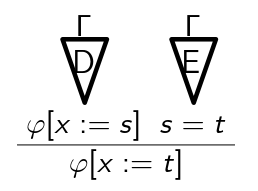
\includegraphics[width=\linewidth]{Assets/Logik-gleiches-für-gleiches-ausführlich.png)
  }

  Gleiches-für-Gleiches (Kurzform)
  %\includegraphics[width=\linewidth]{Assets/Logik-gleiches-für-gleiches-kurz.png)
  Bedingung: über keine Variable aus $s$ oder $t$ wird in $\varphi$ quantifiziert

  Die folgenden Beispiele zeigen, dass wir bereits jetzt die üblichen Eigenschaften der Gleichheit (Symmetrie, Transitivität, Einsetzen) folgern können.

  Beispiel: Seien $x$ Variable, $s$ Term ohne $x$ und $\varphi=(x=s)$.
  \begin{itemize*}
    \item Da $\varphi$ quantorenfrei ist, sind die Substitutionen $[x:=s]$ und $[x:=t]$ für $\varphi$ zulässig.
    \item Außerdem gelten $\varphi[x:=s] = (s=s)$ und $\varphi[x:=t] = (t=s)$.
    \item Also ist das folgende eine Deduktion: %\includegraphics[width=\linewidth]{Assets/Logik-deduktion-beispiel.png)
    \item Für alle Termesundthaben wir also $\{s=t\}\vdash t=s$.
  \end{itemize*}

  Beispiel: Seien $x$ Variable, $r,s$ und $t$ Terme ohne $x$ und $\varphi=(r=x)$.
  \begin{itemize*}
    \item Da $\varphi$ quantorenfrei ist, sind die Substitutionen $[x:=s]$ und $[x:=t]$ für $\varphi$ zulässig.
    \item Außerdem gelten $\varphi[x:=s]=(r=s)$ und $\varphi[x:=t]=(r=t)$.
    \item Also ist das folgende eine Deduktion: %\includegraphics[width=\linewidth]{Assets/Logik-deduktion-beispiel-2.png)
    \item Für alle Terme $r,s$ und $t$ haben wir also $\{r=s,s=t\}\vdash r=t$.
  \end{itemize*}

  Beispiel: Seien $x$ Variable, $s$ und $t$ Terme ohne $x$,$f$ einstelliges Funktionssymbol und $\varphi=(f(s)=f(x))$.
  \begin{itemize*}
    \item Da $\varphi$ quatorenfrei ist, sind die Substitutionen $[x:=s]$ und $[x:=t]$ für $\varphi$ zulässig.
    \item Außerdem gelten $\varphi[x:=s]=(f(s)=f(s))$ und $\varphi[x:=t]=(f(s)=f(t))$.
    \item Also ist das folgende eine Deduktion: %\includegraphics[width=\linewidth]{Assets/Logik-deduktion-beispiel-3.png)
  \end{itemize*}

  \note{Lemma V1}{Sei $\sum$ eine Signatur, $\Gamma$ eine Menge von $\sum$-Formeln und $\varphi$ eine $\sum$-Formel. Sei weiter $D$ eine Deduktion mit Hypothesen in $\Gamma$ und Konklusion $\varphi$, die die Regeln des natürlichen Schließens der Aussagenlogik, $(R)$ und $(GfG)$ verwendet. Dann gilt $\Gamma\Vdash\varphi$.}

  Beweis: Wir erweitern den Beweis des Korrektheitslemmas bzw. des Lemmas V0, der Induktion über die Größe der Deduktion $D$ verwendete.
  \begin{itemize*}
    \item Wir betrachten nur den Fall, dass $D$ die folgende Form hat: %\includegraphics[width=\linewidth]{Assets/Logik-lemma-v1-beweis.png)
    \item Da dies Deduktion ist, sind die Substitutionen $[x:=s]$ und $[x:=t]$ für $\varphi$
    zulässig, d.h. in $\varphi$ wird über keine Variable aus $s$ oder $t$ quantifiziert.
    \item $E$ und $F$ kleinere Deduktionen $\Rightarrow\Gamma\Vdash\varphi[x:=s]$ und $\Gamma\Vdash s=t$
    \item Seien A $\sum$-Struktur und $\rho$ Variableninterpretation mit $A\Vdash_p\gamma$ für alle $\gamma\in\Gamma$.
    \begin{itemize*}
      \item $\Rightarrow A\Vdash_p\varphi[x:=s]$ und $A\Vdash_p s=t$
      \item $\Rightarrow A\Vdash_{p[x\rightarrow \rho(s)]}\varphi$ und $\rho(s) =\rho(t)$
      \item $\Rightarrow A\Vdash_{p[x\rightarrow \rho(t)]}\varphi$
      \item $\Rightarrow A\Vdash_p \varphi[x:=t]$
    \end{itemize*}
    \item Da $A$ und $\rho$ beliebig waren mit $A\Vdash_p\gamma$ für alle $\gamma\in\Gamma$ haben wir $\Gamma\Vdash\varphi[x:=t]$ gezeigt.
  \end{itemize*}

  \subsubsection{$\forall$ in math. Beweisen}
  Ein mathematischer Beweis einer Aussage "für alle $x$ gilt $\varphi$" sieht üblicherweise so aus:
  "Sei $x$ beliebig, aber fest. Jetzt zeige ich $\varphi$ (hier steckt die eigentliche Arbeit). Da $x$ beliebig war, haben wird "für alle $x$ gilt $\varphi$" gezeigt. qed"

  \note{ $\forall$ -Einführung}{ Sei $D$ eine Deduktion mit Hypothesen in $\Gamma$ und Konklusion $\varphi$ und sei $x$ eine Variable, die in keiner Formel aus $\Gamma$ frei vorkommt. Dann ist das folgende eine Deduktion
    mit Hypothesen in $\Gamma$ und Konklusion $\forall x\varphi: \frac{\phi}{\forall x\varphi}$
    Bedingung: $x$ kommt in keiner Hypothese frei vor}

  \note{Lemma V2}{Sei $\sum$ eine Signatur, $\Gamma$ eine Menge von $\sum$-Formeln und $\varphi$ eine $\sum$-Formel. Sei weiter $D$ eine Deduktion mit Hypothesen in $\Gamma$ und Konklusion $\varphi$, die die Regeln des natürlichen Schließens der Aussagenlogik, (R), (GfG) und ($\forall$ -I) verwendet. Dann gilt $\Gamma\Vdash\varphi$.}

  Beweis: Betrachte die folgende Deduktion $D$
  \begin{itemize*}
    \item Insbesondere ist $x$ keine freie Variable einer Formel aus $\Gamma$ und es gilt nach IV $\Gamma\Vdash\varphi$
    \item Sei nun $A$ $\sum$-Struktur und $\rho$ Variableninterpretation mit $A\Vdash_p y$ für alle $y\in\Gamma$.
    \item Zu zeigen ist $A\Vdash_p \forall x\varphi$:
    \begin{itemize*}
      \item Sei also $a\in U_A$ beliebig.
      \item $\Rightarrow$ für alle $y\in\Gamma$ gilt $A\Vdash_{p[x\rightarrow a]} y$ da $x\not\in FV(y)$ und $A\Vdash_p y$
      \item $\Rightarrow A\Vdash_{\rho[x\rightarrow a]}\varphi$
      \item Da $a\in U_A$ beliebig war, haben wir $A\Vdash_\rho\forall x\varphi$ gezeigt
    \end{itemize*}
    \item Da $A$ und $\rho$ beliebig waren mit $A\Vdash_\rho\Gamma$ für alle $\gamma\in\Gamma$ haben wir also $\Gamma\Vdash\forall x\varphi$ gezeigt.
  \end{itemize*}

  \subsubsection{$\forall$ -Elimination in math. Beweisen}
  Ein mathematischer Beweis einer Aussage "t erfüllt $\varphi$" kann so aussehen:
  "Zunächst zeige ich $\forall x\varphi$ (hier steckt die eigentliche Arbeit). Damit erfüllt insbesondere $t$ die Aussage$\varphi$ , d.h., wir haben "$t$ erfüllt $\varphi$" gezeigt. qed"

  \note{ $\forall$ -Elimination}{Sei $D$ eine Deduktion mit Hypothesen in $\Gamma$ und Konklusion $\forall x\varphi$ und seit Term, so dass Substitution [x:=t] für $\varphi$ zulässig ist.
    Dann ist das folgende eine Deduktion mit Hypothesen in $\Gamma$ und Konklusion $\varphi[x:=t]:\frac{\forall x\varphi}{\varphi[x:=t]}$
    Bedingung: über keine Variable aus $t$ wird in $\varphi$ quantifiziert}

  \note{Lemma V3}{ Sei $\sum$ eine Signatur, $\Gamma$ eine Menge von $\sum$-Formeln und $\varphi$ eine $\sum$-Formel. Sei weiter $D$ eine Deduktion mit Hypothesen in $\Gamma$ und Konklusion $\varphi$, die die Regeln des natürlichen Schließens der Aussagenlogik, (R), (GfG), ($\forall$-I) und ($\forall$-E) verwendet. > Dann gilt $\Gamma\Vdash\varphi$.}

  Beweis: Analog zum Beweis von Lemma V2.

  \subsubsection{$\exists$ in math. Beweisen}
  Ein Beweis von "$\sigma$ gilt" kann so aussehen:
  "Zunächst zeige ich $\exists x\varphi$ (hier steckt Arbeit). Jetzt zeige ich, dass $\sigma$ immer gilt, wenn$\varphi$ gilt (mehr Arbeit). Damit gilt $\sigma$. qed"

  \note{$\exists$ -Elimination}{Sei $\Gamma$ eine Menge von Formeln, die die Variable $x$ nicht frei enthalten und enthalte die Formel $\sigma$  die Variabel $x$ nicht frei. Wenn $D$ eine Deduktion mit Hypothesen in $\Gamma$ und Konklusion $\exists x\varphi$ und $E$ eine Deduktion mit Hypothesen in $\Gamma\cup\{\varphi\}$ und Konklusion $\sigma$ ist, dann ist das folgende eine Deduktion mit Hypothesen in $\Gamma$ und Konklusion $\sigma:\frac{\exists x\varphi \quad\quad \sigma}{\sigma}$

    Bedingung: $x$ kommt in den Hypothesen und in $\sigma$ nicht frei vor.}

  \note{Lemma V4}{Sei $\sigma$ eine Signatur, $\Gamma$ eine Menge von $\sum$-Formeln und $\varphi$ eine $\sigma$ -Formel.
    Sei weiter $D$ eine Deduktion mit Hypothesen in $\Gamma$ und Konklusion $\varphi$, die die Regeln des natürlichen Schließens der Aussagenlogik, (R), (GfG), ($\forall$-I), ($\forall$-E) und ($\exists$-E) verwendet. Dann gilt $\Gamma\Vdash\varphi$.}

  Beweis: Sei $D$ die folgende Deduktion
  \begin{itemize*}
    \item Insbesondere kommt $x$ in den Formeln aus $\Gamma\cup\{\sigma\}$ nicht frei vor. Außerdem gelten nach IV $\Gamma\Vdash\exists x\varphi$ und $\Gamma\cup\{\varphi\}\Vdash\sigma$.
    \item Sei nun $A$ $\sigma$-Struktur und $\rho$ Variableninterpretation mit $A\Vdash_\rho\Gamma$ für alle $\gamma\in\Gamma$.
    \item Zu zeigen ist $A\Vdash_\rho\sigma$:
    \begin{itemize*}
      \item Wegen $A\Vdash_\rho\exists x\varphi$ existiert $a\in U_A$ mit $A\Vdash_{\rho[x\rightarrow a]}\varphi$.
      \item $x$ kommt in Formeln aus $\Gamma$ nicht frei vor $\Rightarrow A\Vdash_{\rho[x\rightarrow a]}\gamma$ für alle $\gamma\in\Gamma$.
      \item Aus $\Gamma\cup\{\varphi\}\Vdash\sigma$ folgt $A\Vdash_{\rho[x\rightarrow a]}\sigma$.
      \item Da $x\not\in FV(\sigma)$ erhalten wir $A\Vdash_\rho \sigma$.
    \end{itemize*}
    \item Da $A$ und $\rho$ beliebig waren mit $A\Vdash_\rho\gamma$ für alle $\gamma\in\Gamma$ haben wir also $\Gamma\Vdash\sigma$ gezeigt.
  \end{itemize*}

  \subsubsection{$\exists$ -Einführung in math. Beweisen}
  Ein mathematischer Beweis einer Aussage "es gibt ein $x$, das $\varphi$ erfüllt" sieht üblicherweise so aus: "betrachte dieses $t$ (hier ist Kreativität gefragt). Jetzt zeige ich, daß $t\varphi$ erfüllt (u.U. harte Arbeit). Also haben wir "es gibt ein $x$, das $\varphi$ erfüllt" gezeigt. qed"

  \note{$\exists$ -Einführung}{Sei die Substitution $[x:=t]$ für die Formel $\varphi$ zulässig.
    Sei weiter $D$ eine Deduktion mit Hypothesen in $\Gamma$ und Konklusion $\varphi[x:=t]$.
    Dann ist das folgende eine Deduktion mit Hypothesen in $\Gamma$ und Konklusion $\exists x\varphi:\frac{\varphi[x:=t]}{\exists x\varphi}$

    Bedingung: über keine Variable in $t$ wird in $\varphi$ quantifiziert}

  \note{Korrektheitslemma für das natürliche Schließen in der Prädikatenlogik}{
    Sei $\sigma$ eine Signatur, $\Gamma$ eine Menge von $\sum$-Formeln und $\varphi$ eine $\sigma$ -Formel.
    Sei weiter $D$ eine Deduktion mit Hypothesen in $\Gamma$ und Konklusion $\varphi$, die die Regeln des natürlichen Schließens der Aussagenlogik, (R), (GfG), ($\forall$-I), ($\forall$-E), ($\exists$ -E) und ($\exists$ -I) verwendet. Dann gilt $\Gamma\Vdash\varphi$.}

  Beweis: analog zu obigen Beweisen.

  \subsubsection{Regeln des natürlichen Schließens (Erweiterung)}
  \begin{itemize*}
    \item ($R$): $\frac{}{t=t}$
    \item (GfG): $\frac{\varphi[x:=s] \quad\quad s=t}{\varphi[x:=t]}$ (über keine Variable aus $s$ oder $t$ wird in $\varphi$ quantifiziert)
    \item ($\forall$-I): $\frac{\varphi}{\forall x\varphi}$ (x nicht frei in Hypothesen)
    \item ($\forall$-E): $\frac{\forall x\varphi}{\varphi[x:=t]}$ (über keine Variable aus $t$ wird in $\varphi$ quantifiziert)
    \item ($\exists$-I): $\frac{\varphi [x:=t]}{\exists x\varphi}$ (über keine Variable aus $t$ wird in $\varphi$  quantifiziert)
    \item ($\exists$-I): $\frac{\exists x\varphi\quad\quad \sigma}{\sigma}$ ($x$ kommt in Hypothesen und $\sigma$ nicht frei vor)
  \end{itemize*}

  \note{Definition}{Für eine Menge $\Gamma$ von $\sum$-Formeln und eine $\sum$-Formel $\varphi$ schreiben wir $\Gamma\vdash\varphi$ wenn es eine Deduktion gibt mit Hypothesen in $\Gamma$ und Konklusion $\varphi$. Wir sagen "$\varphi$ ist eine syntaktische Folgerung von $\Gamma$".
    Eine Formel $\varphi$ ist ein Theorem, wenn $\varnothing\vdash\varphi$ gilt.}

  Bemerkung: $\Gamma\vdash\varphi$ sagt (zunächst) nichts über den Inhalt der Formeln in $\Gamma\cup\{\varphi\}$ aus, sondern nur über den Fakt, dass $\varphi$ mithilfe des natürlichen Schließens aus den Formeln aus $\Gamma$ hergeleitet werden kann.
  Ebenso sagt "$\varphi$ ist Theorem" nur, dass $\varphi$ abgeleitet werden kann, über "Wahrheit" sagt dieser Begriff (zunächst) nichts aus.
  Wir haben aber "en passant" das folgende gezeigt:

  \note{Korrektheitssatz}{Für eine Menge von $\sum$-Formeln $\Gamma$ und eine $\sum$-Formel $\varphi$ gilt $\Gamma\vdash\varphi \Rightarrow \Gamma\Vdash\varphi$.}

  Beispiel: Seien $\varphi$ Formel und $x$ Variable. Dann gelten $\{\lnot\exists x\varphi\}\Vdash\forall x\lnot\varphi$ und $\{\forall x\lnot\varphi\}\Vdash\lnot\exists x\varphi$.
  \begin{itemize*}
    \item Beweis: %\includegraphics[width=\linewidth]{Assets/Logik-korrekheitssatz.png)
  \end{itemize*}

  Beispiel: Seien $\varphi$ Formel und $x$ Variable. Dann gelten $\{\lnot\forall x\varphi\}\Vdash \exists x\lnot\varphi$ und $\{\exists x\lnot\varphi\}\Vdash\lnot\forall x\varphi$.
  \begin{itemize*}
    \item Beweis: %\includegraphics[width=\linewidth]{Assets/Logik-beispiel-korrekheitssatz.png)
  \end{itemize*}

  \subsection{Vollständigkeit}
  Können wir durch mathematische Beweise zu allen korrekten Aussagen kommen?
  Können wir durch das natürliche Schließen zu allen korrekten Aussagen kommen?

  Existiert eine Menge $\Gamma$ von $\sum$-Formeln und eine $\sum$-Formel $\varphi$ mit $\Gamma\Vdash\varphi$ und $\Gamma\not\vdash\varphi$?

  Frage: Gilt $\Gamma\Vdash\varphi \Rightarrow \Gamma\vdash\varphi$ bzw. $\varphi$ ist allgemeingültig $\Rightarrow\varphi$ ist Theorem?

  Plan:
  \begin{itemize*}
    \item z.z. ist $\Gamma\Vdash\varphi \Rightarrow \Gamma\vdash\varphi$.
    \item dies ist äquivalent zu $\Gamma\not\vdash\varphi \Rightarrow \Gamma\not\Vdash\varphi$.
    \item hierzu geht man folgendermaßen vor:
    \begin{itemize*}
      \item $\Gamma\not\vdash\varphi$
      \item $\Leftrightarrow \Gamma\cup\{\lnot\varphi\}$ konsistent
      \item $\Rightarrow \exists\Delta\supseteq\Gamma\cup\{\lnot\varphi\}$ maximal konsistent
      \item $\Rightarrow \exists\Delta^+ \supseteq\Delta$ maximal konsistent mit Konkretisierung
      \item $\Rightarrow \Delta^+$ erfüllbar
      \item $\Rightarrow \Delta$ erfüllbar
      \item $\Rightarrow \Gamma\cup\{\lnot\varphi\}$ erfüllbar
      \item $\Leftrightarrow \Gamma\cup\{\lnot\varphi\}$
    \end{itemize*}
  \end{itemize*}

  \note{Definition}{Eine Menge $\Delta$ von Formeln hat Konkretisierungen, wenn für alle $\exists x\varphi\in\Delta$ ein variablenloser Term $t$ existiert mit $\varphi[x:=t]\in\Delta$.}

  \note{Satz}{Sei $\Delta$ eine maximal konsistente Menge von $\sum$-Formeln. Dann existiert eine Signatur $\sum^+ \supseteq\sum$ und eine maximal konsistente Menge von $\sum^+$-Formeln mit Konkretisierungen, so dass $\Delta\subseteq\Delta^+$.}

  Beweis: Wir konstruieren induktiv Signaturen $\sum_n$, maximal konsistente Menge von $\sum_n$-Formeln $\Delta_n$ und konsistente Mengen von $\sum_{n+1}$-Formeln $\Delta'_{n+1}$ mit
  \begin{itemize*}
    \item $\sum =\sum_0 \subseteq\sum_1 \subseteq\sum_2...$ und
    \item $\Delta = \Delta_0 \subseteq \Delta'_1 \subseteq\Delta_1 \subseteq\Delta'_2...$
    und setzen dann
    \item $\sum^+ =\bigcup_{n\geq 0} \sum_n$ und $\Delta^+ = \bigcup_{n\geq 0} \Delta_n$
  \end{itemize*}

  \begin{enumerate*}
    \item IA: $\sum_0 := \sum$ , $\Delta_0:=\Delta$
    \item IV: Sei $n\geq 0$ und $\Delta_n$ maximal konsistente Menge von $\sum_n$-Formeln. $\psi=\exists x\varphi$, ein "neues" Konstantensymbol $c_{\psi}$
    \item IS: $\sum_{n+1}$: alle Symbole aus $\sum_n$ und, für jede Formel $\psi\in\Delta_n$ der Form $\Delta'_{n+1}:= \Delta_n\cup\{\varphi[x:=c_{\psi}]|\psi=\exists x\varphi\in\Delta_n\}$
    \begin{itemize*}
      \item ohne Beweis: $\Delta'_{n+1}$ ist konsistent
      \item Idee: Ist $\varphi$ $\sum_n$-Formel mit $\Delta'_{n+1}\vdash\varphi$, so gilt $\Delta_n\vdash\varphi$.
      \item Konsistenz von $\Delta'_{n+1}$ folgt mit $\varphi=\bot$
      \item Analog zum Satz aus Vorlesung 4 existiert $\Delta_{n+1}\supseteq \Delta'_{n+1}$ maximal konsistent
    \end{itemize*}
    \begin{itemize*}
      \item Damit ist die Konstruktion der Signaturen $\sum_n$ und der maximal konsistenten Mengen $\Delta_n$  von $\sum_n$-Formeln abgeschlossen.
      \item noch z.z.: $\Delta^+$ hat Konkretisierungen und ist maximal konsistent
      \begin{itemize*}
        \item $\Delta^+$ hat Konkretisierungen: Sei $\psi=\exists x\varphi\in\Delta^+$
        \begin{itemize*}
          \item $\Rightarrow$ es gibt $n\geq 0$ mit $\psi\in\Delta_n$
          \item $\Rightarrow \varphi[x:=c_{\psi}]\in\Delta'_{n+1}\subseteq \Delta_{n+1}\subseteq\Delta^+$.
        \end{itemize*}
        \item Konsistenz: (indirekt) angenommen, $\Delta^+\vdash\bot$
        \begin{itemize*}
          \item Da jede Deduktion endlich ist, existiert $\Gamma\subseteq\Delta^+$ endlich mit $\Gamma\vdash\bot$.
          \item $\Rightarrow$ es gibt $n\geq 0$ mit $\Gamma\subseteq\Delta_n$
          \item $\Rightarrow \Delta_n\vdash\bot$ - im Widerspruch zur Konsistenz von $\Delta_n$.
        \end{itemize*}
        \item maximale Konsistenz: (indirekt) angenommen, $\Delta^+$ ist nicht maximal konsistent
        \begin{itemize*}
          \item $\Rightarrow$ es gibt $\Gamma\not\subseteq\Delta^+$ konsistent
          \item $\Rightarrow$ es gibt $\varphi\in\Gamma\backslash\Delta^+$
          \item $\Rightarrow$ $\Delta^+\cup\{\varphi\}\subseteq\Gamma$ konsistent
          \item $\varphi$ ist $\sum^+$-Formel $\Rightarrow$ es gibt $n\geq 0$, so dass $\varphi$ eine $\sum_n$-Formel ist.
          \item $\Delta_n$ maximal konsistente Menge von $\sum_n$-Formeln
          \item $\Rightarrow$ $\varphi\in\Delta_n\subseteq\Delta^+$ oder $\lnot\varphi\in\Delta_n\subseteq\Delta^+$
          \item $\Rightarrow$ $\lnot\varphi\in\Delta^+\subseteq\Gamma$
          \item Also $\varphi,\lnot\varphi\in\Gamma$, im Widerspruch zur Konsistenz von $\Gamma$.
        \end{itemize*}
      \end{itemize*}
    \end{itemize*}
  \end{enumerate*}

  \note{Satz}{Sei $\Delta^+$ maximal konsistente Menge von $\sum^+$-Formeln mit Konkretisierungen. Dann ist $\Delta^+$ erfüllbar.}

  Beweisidee: Sei $T$ die Menge der variablenlosen $\sum^+$-Terme. Auf $T$ definieren wir eine Äquivalenzrelation $\sim$ durch $s\sim t\Leftrightarrow \Delta^+\vdash(s=t)\Leftrightarrow (s=t)\in\Delta^+$
  Sei $A$ die folgende $\sum^+$-Struktur:
  \begin{itemize*}
    \item $U_A:=T/\sim$ ist die Menge der $\sim$-Äquivalenzklassen
    \item $R^A=\{([t_1],...,[t_k])|t_1 ,...,t_k\in T,R(t_1,...,t_k)\in\Delta^+\}$ für alle Relationssymbole R aus $\sum^+$
    \item $f^A([t_1],...,[t_k]) = [f(t_1,...,t_k)]$ für alle $t_1,...,t_k\in T$ und alle Funktionssymbole $f$ aus $\sum^+$ (Bemerkung: dies ist wohldefiniert)
    Dann gilt tatsächlich $A\Vdash\Delta^+$.
  \end{itemize*}

  \note{Satz: Vollständigkeitssatz der Prädikatenlogik }{Sei $\Gamma$ eine Menge von $\sum$-Formeln und $\varphi$ eine $\sum$-Formel. Dann gilt $\Gamma\Vdash\varphi \Rightarrow \Gamma\vdash\varphi$.
    Insbesondere ist jede allgemeingültige Formel ein Theorem.}

  Beweis:indirekt
  \begin{itemize*}
    \item $\Gamma\not\vdash\varphi$
    \item $\Gamma\cup\{\lnot\varphi\}$ konsistent
    \item $\Gamma\cup\{\lnot\varphi\}$ erfüllbar
    \item $\exists\Delta\supseteq\Gamma\cup\{\lnot\varphi\}$ maximal konsistent
    \item $\exists\Delta^+\supseteq\Delta$ maximal konsistent mit Konkretisierungen
    \item $\Delta^+$ erfüllbar
    \item $\Delta$ erfüllbar
    \item $\Gamma\not\Vdash\varphi$
  \end{itemize*}

  Bemerkung
  \begin{itemize*}
    \item Dieser Satz ist (im wesentlichen) der berühmte Gödelsche Vollständigkeitssatz von 1930.
    \item Der obige Beweis wurde von Leon Henkin 1949 veröffentlicht.
  \end{itemize*}

  Wir haben gleichzeitig gezeigt:
  \note{Satz}{Sei $\Gamma$ höchstens abzählbar unendliche und konsistente Menge von Formeln. Dann hat $\Gamma$ ein höchstens abzählbar unendliches Modell.}

  Beweis: $\Gamma$ konsistent heißt $\Gamma\not\vdash\bot$. Obiger Beweis gibt ein Modell $A$ von $\Gamma\cup\{\lnot\bot\}$ an. Wir zeigen, dass diese Struktur $A$ höchstens abzählbar unendlich ist:
  \begin{itemize*}
    \item Sei $\sum$ Signatur der Relations- und Funktionssymbole aus $\Gamma$.
    \item $|\Gamma|\leq \mathbb{N}_0 \Rightarrow |\sum|\leq \mathbb{N}_0$
    \item $\Rightarrow |\sum_n|\leq \mathbb{N}_0$ und $|\Delta_n|\leq \mathbb{N}_0$ für alle $n\geq 0$
    \item $\Rightarrow |\sum^+|,|\Delta^+| \leq\mathbb{N}_0$
    \item $\Rightarrow |T| \leq\mathbb{N}_0$
    \item $\Rightarrow A$ hat $\leq\mathbb{N}_0$ viele Elemente
    \item $\Rightarrow \Gamma\cup\{\lnot\bot\}$ hat ein höchstens abzählbar unendliches Modell
    \item $\Rightarrow \Gamma$ hat ein höchstens abzählbar unendliches Modell
  \end{itemize*}

  \subsection{Vollständigkeit und Korrektheit für die Prädikatenlogik}
  \note{Satz}{Seien $\Gamma$ eine Menge von $\sum$-Formeln und $\varphi$ eine $\sum$-Formel. Dann gilt $\Gamma\vdash\varphi\Leftrightarrow \Gamma\Vdash\varphi$.
    Insbesondere ist eine $\sum$-Formel genau dann allgemeingültig, wenn sie ein Theorem ist.}

  Beweis: Folgt unmittelbar aus Korrektheitssatz und Vollständigkeitssatz.

  \subsubsection{Folgerung 1: Kompaktheit}
  \note{Satz}{Seien $\Gamma$ eine u.U. unendliche Menge von $\sum$-Formeln und $\varphi$ eine $\sum$-Formel mit $\Gamma\Vdash\varphi$. Dann existiert $\Gamma'\subseteq\Gamma$ endlich mit $\Gamma'\Vdash\varphi$.}

  Beweis: $\Gamma\Vdash\varphi$
  \begin{itemize*}
    \item $\Gamma\vdash\varphi$ (nach dem Vollständigkeitssatz)
    \item es gibt Deduktion von $\varphi$ mit Hypothesen $\gamma_1,...,\gamma_n\in\Gamma$
    \item $\Gamma'=\{\gamma_1,...,\gamma_n\}\subseteq\Gamma$ endlich mit $\Gamma'\vdash\varphi$
    \item $\Gamma'\vdash\varphi$ (nach dem Korrektheitssatz).
  \end{itemize*}

  \note{Folgerung (Kompaktheits- oder Endlichkeitssatz)}{Sei $\Gamma$ eine u.U. unendliche Menge von $\sum$-Formeln. Dann gilt $\Gamma$ erfüllbar $\Leftrightarrow \forall\Gamma'\subseteq\Gamma$ endlich: $\Gamma'$ erfüllbar}

  Beweis:
  \begin{itemize*}
    \item $\Gamma$ unerfüllbar
    \item $\Leftrightarrow \Gamma\cup\{\lnot\bot\}$ unerfüllbar
    \item $\Leftrightarrow \Gamma\Vdash\bot$
    \item $\Leftrightarrow$ es gibt $\Gamma'\subseteq\Gamma$ endlich: $\Gamma'\Vdash\bot$
    \item $\Leftrightarrow$ es gibt $\Gamma'\subseteq\Gamma$ endlich: $\Gamma'\cup\{\lnot\bot\}$ unerfüllbar
    \item $\Leftrightarrow$ es gibt $\Gamma'\subseteq\Gamma$ endlich: $\Gamma'$ unerfüllbar
  \end{itemize*}

  \note{Satz}{Sei $\Delta$ eine u.U. unendliche Menge von $\sum$-Formeln, so dass für jedes $n\in\mathbb{N}$ eine endliche Struktur $A_n$ mit $A_\Vdash\Delta$ existiert, die wenigstens $n$ Elemente hat.
    Dann existiert eine unendliche Struktur $A$ mit $A\Vdash\Delta$.}

  Beweis: für $n\in\mathbb{N}$ setze $\varphi_n=\exists x_1 \exists x_2 ...\exists x_n \bigwedge_{1\leq i< j \leq n} x_i \not= x_j$
  \begin{itemize*}
    \item und $\Gamma =\Delta\cup\{\varphi_n | n\geq 0\}$.
    \item Für $\Gamma'\subseteq\Gamma$ endlich existiert $n\in\mathbb{N}$ mit $\varphi_m\not\in\Gamma'$ für alle $m\geq n$
    \item $\Rightarrow A_n\Vdash\Gamma'$, d.h. jede endliche Teilmenge von $\Gamma$ ist erfüllbar.
    \item $\Rightarrow$ es gibt Struktur $A$ mit $A\Vdash\Gamma$
    \item $\Rightarrow$ A hat $\geq n$ Elemente (für alle $n\in\mathbb{N}$)
  \end{itemize*}

  \subsubsection{Folgerung 2: Löwenheim-Skolem}
  Frage: Gibt es eine Menge $\Gamma$ von $\sum$-Formeln, so dass für alle Strukturen $A$ gilt: $A\Vdash\Gamma \Leftrightarrow A\cong (\mathbb{R},+,*, 0 , 1 )$?

  \note{Satz von Löwenheim-Skolem}{Sei $\Gamma$ erfüllbare und höchstens abzählbar unendliche Menge von $\sum$-Formeln. Dann existiert ein höchstens abzählbar unendliches Modell von $\Gamma$.}

  Beweis:
  \begin{itemize*}
    \item $Gamma$ erfüllbar $\Rightarrow \Gamma\not\Vdash\bot$
    \item $\Rightarrow$ $\Gamma\not\vdash\bot$, d.h. $\Gamma$ konsistent
    \item $\Rightarrow \Gamma$ hat ein höchstens abzählbar unendliches Modell.
  \end{itemize*}

  Die Frage auf der vorherigen Folie muß also verneint werden:
  \begin{itemize*}
    \item angenommen, $\Gamma$ wäre eine solche Menge
    \item $\Rightarrow |\Gamma|\leq \mathbb{N}_0$
    \item $\Rightarrow \Gamma$ hat ein höchstens abzählbar unendliches Modell $A$
    \item $\Rightarrow A\not\cong (\mathbb{R},+,*, 0 , 1 )$
  \end{itemize*}


  \subsubsection{Folgerung 3: Semi-Entscheidbarkeit}
  \note{Satz}{Die Menge der allgemeingültigen $\sum$-Formeln ist semi-entscheidbar.}

  Beweis:Sei$\varphi$ $\sum$-Formel. Dann gilt
  \begin{itemize*}
    \item $\varphi$ allgemeingültig
    \item $\Leftrightarrow \varphi$ Theorem
    \item $\Leftrightarrow$ Es gibt hypothesenlose Deduktion mit Konklusion $\varphi$
  \end{itemize*}

  Ein Semi-Entscheidungsalgorithmus kann also folgendermaßen vorgehen:
  Teste für jede Zeichenkette $w$ nacheinander, ob sie hypothesenlose Deduktion mit Konklusion $\varphi$ ist. Wenn ja, so gib aus "$\varphi$ ist allgemeingültig". Ansonsten gehe zur nächsten Zeichenkette über.

  \subsubsection{Der Satz von Church}
  Jetzt zeigen wir, daß dieses Ergebnis nicht verbessert werden kann: Die Menge der allgemeingültigen $\sum$-Formeln ist nicht entscheidbar.
  Wegen $\varphi$ allgemeingültig $\Leftrightarrow\lnot\varphi$ unerfüllbar reicht es zu zeigen, dass die Menge der erfüllbaren Sätze nicht entscheidbar ist.
  Genauer zeigen wir dies sogar für "Horn-Formeln":

  \note{Definition}{Eine Horn-Formel ist eine Konjunktion von $\sum$-Formeln der Form $\forall x_1 \forall x_2 ...\forall x_n((\lnot\bot \wedge\alpha_1\wedge\alpha_2\wedge...\wedge\alpha_m)\rightarrow\beta)$, wobei $\alpha_1,...,\alpha_m$ und $\beta$ atomare $\sum$-Formeln sind.}

  Unser Beweis reduziert die unentscheidbare Menge PCP auf die Menge der erfüllbaren Horn-Formeln.

  Im folgenden sei also $I=((u_1,v_1),(u_2,v_2),...,(u_k,v_k))$ ein Korrespondenzsystem und $A$ das zugrundeliegende Alphabet.
  Hieraus berechnen wir eine Horn-Formel $\varphi_I$, die genau dann erfüllbar ist, wenn $I$ keine Lösung hat.
  Wir betrachten die Signatur $\sum= (\Omega,Rel,ar)$ mit
  \begin{itemize*}
    \item $\Omega=\{e\}\cup\{f_a|a\in A\}$ mit $ar(e) =0$ und $ar(f_a) =1$ für alle $a\in A$.
    \item $Rel=\{R\}$ mit $ar(R)=2$.
  \end{itemize*}

  Zur Abkürzung schreiben wir $f_{a_1 a_2 ...a_n} (x)$ für $f_{a_1}(f_{a_2}(...(f_{a_n}(x))...))$ für alle $a_1,a_2,...,a_n\in A$ und $n\geq 0$ (insbes. steht $f_{\epsilon}(x)$ für $x$).

  Zunächst betrachten wir die folgende Horn-Formel $\psi_I$:
  \begin{itemize*}
    \item $\wedge \bigwedge_{1\leq j \leq k}^{R(e,e)} \forall x,y(R(x,y)\rightarrow R(f_{u_j}(x),f_{v_j}(y)))$
    \item $\wedge \bigwedge_{a\in A} \forall x(e=f_a(x)\rightarrow \bot)$
  \end{itemize*}

  Beispiel: Betrachte die $\sum$-Struktur $A$ mit Universum $U_A=A^*$
  \begin{itemize*}
    \item $e^A=\epsilon$
    \item $f_a^A(u) =au$
    \item $R^A=\{(u_{i1} u_{i2} ...u_{in},v_{i1} v_{i2} ...v_{in})|n\geq 0 , 1\geq i_1,i_2,...,i_n\geq k\}$
    \item Für $u,v\in A^*$ gilt $f_u^A(v) =uv$.
    \item Dann gilt $A\Vdash \psi_I$.
  \end{itemize*}

  \note{Lemma}{Angenommen, das Korrespondenzsystem $I$ hat keine Lösung. Dann ist die Horn-Formel $\varphi_I=\psi_I \wedge \forall x(R(x,x)\rightarrow x=e)$ erfüllbar.}

  Beweis: Sei $A$ die obige Struktur mit $A\Vdash\psi_I$.
  \begin{itemize*}
    \item Um $A\Vdash\forall x(R(x,x)\rightarrow x=e)$ zu zeigen, sei $w\in U_A$ beliebig mit $(w,w)\in R^A$.
    \item Die Definition von $R^A$ sichert die Existenz von $n\geq 0$ und $1\leq i_1,i_2,...,i_n\leq k$ mit $u_{i1} u_{i2}...u_{in}=w=v_{i1} v_{i2} ...v_{in}$.
    \item Da $I$ keine Lösung hat, folgt $n=0$ und damit $w=\epsilon$.
  \end{itemize*}

  \note{Lemma}{Sei $B$ Struktur mit $B\Vdash\psi_I$. Dann gilt $(f_{u_{i_1} u_{i_2} ...u_{i_n}}^B (e^B),f_{v_{i_1} v_{i_2}...v_{i_n}}^B(e^B))\in R^B$ für alle $n\geq 0, 1\leq i_1,i_2,...,i_n \leq k$.}

  Beweis: per Induktion über $n\geq 0$.
  \begin{itemize*}
    \item IA: für $n=0$ gelten $f_{u_{i_1} u_{i_2} ...u_{i_n}}^B(e^B) =e^B$ und $f_{v_{i_1} v_{i_2}...v_{i_n}}^B(e^B) =e^B$
    \begin{itemize*}
      \item und damit $(f_{u_{i_1} u_{i_2} ...u_{i_n}}^B(e^B), f_{v_{i_1} v_{i_2}...v_{i_n}}^B(e^B) \in R^B$
      \item wegen $B\Vdash\psi_I$.
    \end{itemize*}
    \item IS: Seien $n>0$ und $1\leq i_1 ,i_2 ,...,i_n\leq k$.
    \begin{itemize*}
      \item Mit $u=u_{i2} u_{i3} ...u_{in}$ und $v=v_{i2} v_{i3} ...v_{in}$ gilt nach IV $(f_u^B(e^B),f_v^B(e^B))\in R^B$. Wegen $B\Vdash\psi_I$ folgt $f_{u_{i_1} u_{i_2} ...u_{i_n}}^B(e^B), f_{v_{i_1} v_{i_2}...v_{i_n}}^B(e^B) = (f_{u_{i1}}^B (f_u^B(e^B)),f_{v_{i1}}^B (f_v^B(e^B)))\in RB$.
    \end{itemize*}
  \end{itemize*}

  \note{Lemma}{Angenommen, $(i_1,...,i_n)$ ist eine Lösung von $I$. Dann ist die $\sum$-Formel $\varphi_I$ unerfüllbar.}

  \note{Satz}{Die Menge der unerfüllbaren Horn-Formeln ist nicht entscheidbar.}

  Beweis: Die Abbildung $I\rightarrow\varphi_I$ ist berechenbar.

  Nach den vorherigen Lemmata ist sie eine Reduktion von PCP auf die Menge der unerfüllbaren Horn-Formeln. Da PCP unentscheidbar ist (vgl. Automaten, Sprachen und Komplexität), ist die Menge der unerfüllbaren Horn-Formeln unentscheidbar.

  \note{Folgerung (Church 1936)}{Die Menge der allgemeingültigen $\sum$-Formeln ist nicht entscheidbar.}

  Beweis: Eine $\sum$-Formel $\varphi$ ist genau dann unerfüllbar, wenn $\lnot\varphi$ allgemeingültig ist. Also ist $\varphi\rightarrow\lnot\varphi$ eine Reduktion der unentscheidbaren Menge der unerfüllbaren $\sum$-Formeln auf die Menge der allgemeingültigen $\sum$-Formeln, die damit auch unentscheidbar ist.

  Allgemeingültige $\sum$-Formeln gelten in allen Strukturen. Was passiert, wenn wir uns nur auf "interessante" StrukturenAeinschränken (z.B. auf eine konkrete), d.h. wenn wir die Theorie $Th(A)$ von $A$ betrachten?


  \subsection{Theorie der natürlichen Zahlen}
  \note{Definition}{Sei $A$ eine Struktur. Dann ist $Th(A)$ die Menge der prädikatenlogischen $\sum$-Formeln $\varphi$ mit $A\Vdash\varphi$. Diese Menge heißt die(elementare) Theorie von $A$.}

  Beispiel: Sei $N= (N,\leq,+,*, 0 , 1 )$. Dann gelten
  \begin{itemize*}
    \item $(\forall x\forall y:x+y=y+x)\in Th(N)$
    \item $(\forall x\exists y:x+y= 0 )\not\in Th(N)$
    \item aber $(\forall x\exists y:x+y= 0 )\in Th((Z,+, 0 ))$.
  \end{itemize*}

  \note{Lemma}{Die Menge $Th(N)$ aller Sätze $\varphi$ mit $N\Vdash\varphi$ ist nicht entscheidbar.}

  \note{Zahlentheoretisches Lemma}{Für alle $n\in N,x_0,x_1,...,x_n\in N$ existieren $c,d\in N$, so dass für alle $0\leq i\leq n$ gilt: $x_i=c\ mod ( 1 +d*(i+ 1 ))$.}

  Beweis:Setze $m= max\{n,x_0,x_1 ,...,x_n\}$ und $d=2*3*4...(m+1)$. Dann sind die Zahlen $1+d, 1+d*2,..., 1 +d*(n+1)$ paarweise teilerfremd. Nach dem Chinesischen Restsatz folgt die Existenz
  einer natürlichen Zahl $c$.

  Bemerkung: Es gibt $\sum$-Formeln
  \begin{itemize*}
    \item $mod(x_1,x_2 ,y)$ mit $N\Vdash_{\alpha} mod \Leftrightarrow \alpha (x_1) mod\alpha (x_2) =\alpha (y)$.
    \item $\gamma(x_1 ,x_2 ,x_3 ,y)$ mit $N\Vdash_{\alpha} \gamma\Leftrightarrow \alpha(x_1) mod(1+\alpha(x_2)*(\alpha (x3)+1)) =\alpha (y)$.
  \end{itemize*}

  \note{Satz}{Sei $A$ eine Struktur, so dass $Th(A)$ semi-entscheidbar ist. Dann ist $Th(A)$ entscheidbar.}

  \note{Korollar}{Die Menge $TH(N)$ der Aussagen $\varphi$ mit $N\Vdash\varphi$ ist nicht semi-entscheidbar.}

  \note{Korollar (1. Gödelscher Unvollständigkeitssatz)}{Sei $Gamma$ eine semi-entscheidbare Menge von Sätzen mit $N\Vdash\gamma$ für alle $\gamma\in\Gamma$. Dann existiert ein Satz $\varphi$ mit $\Gamma\not\vdash\varphi$ und $\Gamma\not\vdash\lnot\varphi$ (d.h. "$\Gamma$ ist nicht vollständig").}

  \subsection{2. Semi Entscheidungsverfahren für allgemeingültige Formeln}
  bekanntes Verfahren mittels natürlichem Schließen: Suche hypothesenlose Deduktion mit Konklusion $\psi$.

  Jetzt alternatives Verfahren, das auf den Endlichkeitssatz der Aussagenlogik zurückgreift:
  \begin{itemize*}
    \item Berechne aus $\sum$-Formel $\psi$ eine Menge E von aussagenlogischen Formeln mit $E$ unerfüllbar $\Leftrightarrow\lnot\psi$ unerfüllbar $\Leftrightarrow\psi$ allgemeingültig
    \item Suche endliche unerfüllbare Teilmenge $E'$ von $E$
  \end{itemize*}

  Kern des Verfahrens ist es also, aus $\sum$-Formel $\varphi$ eine Menge $E$ aussagenlogischer Formeln zu berechnen mit $\varphi$ unerfüllbar $\Leftrightarrow$ E unerfüllbar.

  Hierzu werden wir die Formel $\varphi$ zunächst in zwei Schritten (Gleichungsfreiheit und Skolem-Form) vereinfachen, wobei die Formel erfüllbar bzw unerfüllbar bleiben muss.

  \note{Definition}{Zwei $\sum$-Formeln $\varphi$ und $\psi$ heißen erfüllbarkeitsäquivalent, wenn gilt: $\varphi$ ist erfüllbar $\Leftrightarrow\psi$ ist erfüllbar}

  Unsere Vereinfachungen müssen also erfüllbarkeitsäquivalente Formeln liefern.

  \subsubsection{Elimination von Gleichungen}
  \note{Definition}{Eine $\sum$-Formel ist gleichungsfrei, wenn sie keine Teilformel der Form $s=t$ enthält. }

  Ziel: aus einer $\sum$ Formel $\varphi$ soll eine erfüllbarkeitsäquivalente gleichungsfreue Formel $\varphi'$ berechnet werden

  Bemerkung: Man kann i.a. keine äquivalente gleichungsfreie Formel $\varphi'$ angeben, da es eine solche z.B. zu $\varphi=(\forall x\forall y:x=y)$ nicht gibt.

  Idee: Die Formel $\varphi'$ entsteht aus $\varphi$, indem alle Teilformeln der Form $x=y$ durch $GI(x,y)$ ersetzt werden, wobei $GI$ ein neues Relationssymbol ist.

  Notationen
  \begin{itemize*}
    \item Sei $\sum=(\Omega,Rel,ar)$ endliche Signatur und $\varphi$ $\sum$-Formel
    \item $\sum_{GI} = (\Omega, Rel\bigcup^+\{GI\},ar_{GI})$ mit $ar_{GI}(f)$ für alle $f\in\Omega\cup Rel$ und $ar_{GI}(GI)=2$
    \item Für eine $\sum$-Formel $\varphi$ bezeichnet $\varphi_{GI}$ die $\sum_{GI}$-Formel, die aus $\varphi$ entsthet, indem alle Vorkommen und Teilformen $s=t$ durch $GI(s,t)$ ersetzt werden.
  \end{itemize*}

  Behauptung: $\varphi$ erfüllbar $\Rightarrow \varphi_{GI}$ erfüllbar

  Behauptung: es gilt nicht $\varphi$ erfüllbar $\Leftarrow\varphi_{GI}$ erfüllbar

  \note{Definition}{Sei A eine $\sum$-Struktur und $\sim$ eine binäre Relation auf $U_A$. Die Relation $\sim$ heißt Kongruenz auf A, wenn gilt:
    \begin{itemize*}
      \item $\sim$ ist eine Äquivalentrelation (d.h. reflexiv, transitiv und symmetrisch)
      \item für alle $f\in\Omega$ mit $k=ar(f)$ und alle $a_1,b_1,...,a_k,b_k\in U_A$ gilt $a_1\sim b_1,a_2\sim b_2,...,a_k\sim b_k\Rightarrow f^A(a_1,...,a_k)\sim f^A(b_1,...,b_k)$
      \item für alle $R\in Rel$ mit $k=ar(R)$ und alle $a_1,b_1,...,a_k,b_k\in U_A$ gilt $a_1\sim b_1,...,a_k\sim b_k,(a_1,...,a_k)\in R^A\Rightarrow (b_1,...,b_k)\in R^A$.
    \end{itemize*}
  }

  \note{Definition}{Sei $A$ eine $\sum$-Struktur und $\sim$ eine Kongruenz auf A.
    \begin{enumerate*}
      \item Für $a\in U_A$ sei $[a]=\{b\in U_A|a\sim b\}$ die Äquivalenzklasse von a bzgl $\sim$.
      \item Dann definieren wir den Quotienten $B=A\backslash \sim$ von $A$ bzgl $\sim$ wie folgt:
      \begin{itemize*}
        \item $U_B=U_A\backslash\sim = \{[a]|a\in U_A\}$
        \item Für jedes $f\in\Omega$ mit $ar(f)=k$ und alle $a_1,...,a_k\in U_A$ setzten wir $f^B([a_1],...,[a_k])=[f^A(a_1,...,a_k)]$
        \item für jede $R\in Rel$ mit $ar(R)=k$ setzten wir $R^B=\{([a_1],[a_2],...,[a_k])|(a_1,...,a_k)\in R^A\}$
      \end{itemize*}
      \item Sei $p:Var\rightarrow U_A$ Variableninterpretation. Dann definieren die Variableninterpretation $p\backslash\sim: Var\rightarrow U_B:x\rightarrow[p(x)]$.
    \end{enumerate*}
  }

  Veranschaulichung: %\includegraphics[width=\linewidth]{Assets/Logik-variableninterpretation-beispiel.png)

  \note{Lemma 1}{Sei A Struktur, $p:Var\rightarrow U_A$ Variableninterpretation und $\sim$ Kongruenz. Seien weiter $B=A\backslash\sim$ und $p_B=p\backslash\sim$. Dann gilt für jeden Term $:[p(t)]=p_B(t)$}

  Beweis: per Induktion über den Aufbau des Terms t

  \note{Lemma 2}{Sei $A$ $\sum$-Struktur, $\sim$ Kongruenz und $B=A\backslash\sim$. Dann gilt für alle $R\in Rel$ mit $k=ar(R)$ und alle $c_1,...,c_k\in U_A$: $([c_1],[c_2],...,[c_k])\in R^B\Leftrightarrow (c_1,c_2,...,c_k)\in R^A$}

  \note{Satz}{Seien $A$ $\sum_{GI}$-Struktur und $p:Var\rightarrow U_A$ Variableninterpretation, so dass $\sim=GI^A$ Kongruenz auf A ist.
    Seien $B=A\backslash\sim$ und $p_B=p\backslash\sim$.
    Dann gilt für alle $\sum$-Formeln $\varphi: A\Vdash_p \varphi_{GI} \Leftrightarrow B\Vdash_{p_B} \varphi$
  }

  Beweis: per Induktion über den Aufbau der Formel $\varphi$

  \note{Lemma}{Aus einer endlichen Signatur $\sum$ kann ein gleichungsfreuer Horn-Satz $Kong_{\sum}$ über $\sum_{GI}$ berechnet werden, so dass für alle $\sum_{GI}$-Strukturen $A$ gilt: $A\Vdash Kong_{\sum} \Leftrightarrow GI^A$ ist eine Kongruenz}

  \note{Satz}{Aus einer endlichen Signatur $\sum$ und einer $\sum$-Formel $\varphi$ kann eine gleichungsfreie und erfüllbarkeitsäquivalente $\sum_{GI}$-Formel $\varphi'$ berechnet werden. Ist $\varphi$ Horn Formel, so ist auch $\varphi'$ Horn Formel.}

  Beweis: Setzte $\varphi' =\varphi_{GI}\wedge Kong_{\sum}$ und zeige: $\varphi$ erfüllbar $\Leftrightarrow \varphi'$ erfüllbar.

  \subsection{Skolemform}
  Ziel: Jede $\sum$-Formel $\varphi$ ist erfüllbarkeitsäquivalent zu einer $\sum$'-Formel $\varphi'=\forall x_1\forall x_2 ...\forall x_k \psi$, wobei $\psi$ kein Quantoren enthält, $\varphi'$ heißt in Skolemform.

  Bemerkung: Betrachte die Formel $\exists x\exists y E(x,y)$. Es gibt keine Formel in Skolemform, die hierzu äquivalent ist.

  2 Schritte:
  \begin{enumerate*}
    \item Quantoren nach vorne (d.h. Pränexform)
    \item Existenzquantoren eliminieren
  \end{enumerate*}

  \note{Definition}{Zwei $\sum$-Formeln $\varphi$ und $\psi$ sind äquivalent (kurz:$\varphi\equiv\psi$), wenn für alle $\sum$-Strukturen $A$ und alle Variableninterpretationen $\rho$ gilt: $A\Vdash_{\rho}\psi\Leftrightarrow A\Vdash_{\rho}\psi$.}

  \note{Lemma}{Seien $Q\in\{\exists ,\forall\}$ und $\oplus\in\{\wedge,\vee,\rightarrow,\leftarrow\}$. Sei $\varphi= (Qx \alpha)\oplus\beta$ und sei $y$ eine Variable, die weder in $\alpha$ noch in $\beta$ vorkommt. Dann gilt $\varphi \equiv \begin{cases} Qy(\alpha[x:=y]\oplus\beta) \text{ falls } \oplus\in\{\wedge,\vee,\leftarrow\}\\ \forall y(\alpha[x:=y]\rightarrow\beta) \text{ falls } \oplus=\rightarrow,Q=\exists \\ \exists y(\alpha[x:=y]\rightarrow\beta) \text{ falls }\oplus=\rightarrow,Q=\forall\end{cases}$}

  Notwendigkeit der Bedingung "$y$ kommt weder in $\alpha$ noch in $\beta$ vor":
  \begin{itemize*}
    \item $(\exists x:f(x) \not =f(y))\wedge\beta \not\equiv\exists y: (f(y) \not =f(y)\wedge\beta)$
    \item $(\exists x:\lnot P(x))\wedge P(y)\not\equiv \exists y: (\lnot P(y) \wedge P(y))$
  \end{itemize*}

  \note{Lemma}{Seien $Q\in\{\exists,\forall\}$ und $\oplus\in\{\wedge,\vee,\rightarrow,\leftarrow\}$. Sei $\varphi= (Qx\alpha)\oplus\beta$ und sei $y$ eine Variable, die weder in $\alpha$ noch in $\beta$ vorkommt. Dann gilt $\varphi\equiv\begin{cases} Qy(\alpha[x:=y]\oplus\beta) \text{ falls }\oplus\in\{\wedge,\vee,\leftarrow\} \\ \forall y(\alpha[x:=y]\rightarrow\beta) \text{ falls }\oplus=\rightarrow,Q=\exists \\ \exists y(\alpha[x:=y]\rightarrow\beta) \text{ falls }\oplus=\rightarrow,Q=\forall \end{cases}$}

  Beweis: (für den Fall $Q=\exists$ und $\oplus=\wedge$)
  \begin{itemize*}
    \item Seien $A$ $\sum$-Struktur und $\rho$ Variableninterpretation.
    \item Für $a\in U_A$ setze $\rho_a:=\rho[y\rightarrow a]$.
    \item Dann gilt $\rho_a[x\rightarrow \rho_a(y)](z) =\rho[x\rightarrow a](z)$ für alle $z\not=y$
  \end{itemize*}


  Wir erhalten also
  \begin{itemize*}
    \item $A\vdash_\rho (\exists x\alpha)\wedge\beta$
    \item $\Leftrightarrow A\vdash_\rho (\exists x\alpha) $ und $A\vdash_\rho \beta$
    \item $\Leftrightarrow$ (es gibt $a\in U_A$ mit $A\vdash_{\rho[x\rightarrow a]}\alpha$) und (es gilt $A\vdash_\rho \beta$)
    \item $\Leftrightarrow$ es gibt $a\in U_A$ mit ($A\vdash_{\rho[x\rightarrow a]}\alpha$ und $A\vdash_\rho \beta$)
    \item $\Leftrightarrow$ es gibt $a\in U_A$ mit
    \begin{itemize*}
      \item $A\vdash_{\rho_a[x\rightarrow \rho_a(y)]}\alpha$ (da $y$ in $\alpha$ nicht vorkommt)
      \item $A\vdash_{\rho_a} \beta$ (da $y$ in $\beta$ nicht vorkommt)
    \end{itemize*}
    \item $\Leftrightarrow$ es gibt $a\in U_A$ mit
    \begin{itemize*}
      \item $A\vdash_{\rho_a} \alpha[x:=y]$
      \item $A\vdash_{\rho_a} \beta$
    \end{itemize*}
    \item $\Leftrightarrow$ es gibt $a\in U_A$ mit $A\vdash_{\rho[y\rightarrow a]}\alpha[x:=y]\wedge\beta$
    \item $\Leftrightarrow A\vdash_\rho \exists y(\alpha[x:=y]\wedge\beta)$
  \end{itemize*}

  \note{Satz}{Aus einer endlichen Signatur $\sum$ und einer $\sum$-Formel $\varphi$ kann eine äquivalente $\sum$-Formel $\varphi'=Q_1 x_1 Q_2 x_2 ...Q_k x_k \psi$ (mit $Q_i\in\{\exists,\forall\},\psi$ quantorenfrei und $x_i$ paarweise verschieden) berechnet werden. Eine Formel $\varphi'$ dieser Form heißt Pränexform.
    Ist $\varphi$ gleichungsfrei, so ist auch $\varphi'$ gleichungsfrei.}

  Beweis: Der Beweis erfolgt induktiv über den Aufbau von $\varphi$:
  \begin{itemize*}
    \item I.A. $\varphi$ ist atomare Formel: Setze $\varphi'=\varphi$.
    \item I.S.
    \begin{itemize*}
      \item $\varphi=\lnot\psi$ : Nach I.V. kann Formel in Pränexform $\psi\equiv Q_1 x_1 Q_2 x_2 ...Q_m x_m \psi'$ berechnet werden. Mit $\forall=\exists$ und $\exists=\forall$ setze $\varphi'=Q_1 x_1 Q_2 x_2 ...Q_m x_m\lnot\psi'$.
      \item $\varphi=\exists x\psi$: Nach I.V. kann Formel in Pränexform $\psi\equiv Q_1 x_1 Q_2 x_2 ...Q_m x_m \psi'$ berechnet werden. Setze $\varphi'= \begin{cases} \exists x Q_1 x_1 Q_2 x_2 ...Q_m x_m\psi'\text{ falls }x\not\in\{x_1,x_2,...,x_m\}\\ Q_1 x_1 Q_2 x_2 ...Q_m x_m\psi'\text{ sonst}\end{cases}$
      \item $\varphi=\alpha\wedge\beta$: Nach I.V. können Formeln in Pränexform $\alpha\equiv Q_1 x_1 Q_2 x_2 ...Q_mx_m \alpha_0; \beta\equiv Q_1'y_1 Q_2'y_2 ...Q_n'y_n \beta_0$ berechnet werden.
    \end{itemize*}
  \end{itemize*}

  Ziel: Berechnung einer erfüllbarkeitsäquivalenten Formel in Skolemform

  Idee:
  \begin{enumerate*}
    \item wandle Formel in Pränexform um
    \item eliminiere $\exists$-Quantoren durch Einführen neuer Funktionssymbole
  \end{enumerate*}

  Konstruktion: Sei $\varphi=\forall x_1\forall x_2...\forall x_m\exists y\psi$ Formel in Pränexform (u.U. enthält $\psi$ weitere Quantoren). Sei $g\not\in\Omega$ ein neues m-stelliges Funktionssymbol.
  Setze $\varphi'=\forall x_1\forall x_2...\forall x_m \psi[y:=g(x_1,...,x_m)]$.
  Offensichtlich hat $\varphi$'einen Existenzquantor weniger als $\varphi$. Außerdem ist $\varphi'$ keine $\sum$-Formel (denn sie verwendet $g\not\in\Omega$), sondern Formel über einer erweiterten Signatur.

  \note{Lemma}{Die Formeln $\varphi$ und $\varphi'$ sind erfüllbarkeitsäquivalent.}

  Beweis: "$\Leftarrow$" Sei $A'$ Struktur und $\rho'$ Variableninterpretation mit $A'\vdash_{\rho'}\varphi'$. Wir zeigen $A'\vdash_{\rho'}\varphi$. Hierzu seien $a_1,...,a_m\in U_{A'}$ beliebig.

  \note{Satz}{Aus einer Formel $\varphi$ kann man eine erfüllbarkeitsäquivalente Formel $\varphi$ in Skolemform berechnen. Ist $\varphi$ gleichungsfrei, so auch $\varphi$.}

  Beweis: Es kann zu $\varphi$ äquivalente Formel $\varphi_0 =Q_1 x_1 Q_2 x_2 ...Q_{\iota}  x_{\iota}   \psi$ in Pränexform berechnet werden (mit $n\leq {\iota}  $ Existenzquantoren). Durch wiederholte Anwendung des vorherigen Lemmas erhält man Formeln $\varphi_1,\varphi_2,...\varphi_n$ mit
  \begin{itemize*}
    \item $\varphi_i$ und $\varphi_{i+1}$ sind erfüllbarkeitsäquivalent
    \item $\varphi_{i+1}$ enthält einen Existenzquantor weniger als $\varphi_i$
    \item $\varphi_{i+1}$ ist in Pränexform
    \item ist $\varphi_i$ gleichungsfrei, so auch $\varphi_{i+1}$
  \end{itemize*}

  Dann ist $\bar{\varphi}=\varphi_n$ erfüllbarkeitsäquivalente (ggf. gleichungsfreie) Formel in Skolemform.

  \subsection{Herbrand-Strukturen und Herbrand-Modelle}
  Sei $\sum= (\Omega,Rel,ar)$ eine Signatur. Wir nehmen im folgenden an, dass $\Omega$ wenigstens ein Konstantensymbol enthält.

  Das Herbrand-Universum $D(\sum)$ ist die Menge aller variablenfreien $\sum$-Terme.

  Beispiel: $\Omega =\{b,f\}$ mit $ar(b) =0$ und $ar(f) =1$. Dann gilt $D(\sum) =\{b,f(b),f(f(b)),f(f(f(b))),...\}$

  Eine $\sum$-Struktur $A=(UA,(fA)f\in\Omega,(RA)R\in Rel)$ ist eine Herbrand-Struktur, falls folgendes gilt:
  \begin{enumerate*}
    \item $UA=D(\sum)$,
    \item für alle $f\in\Omega$ mit $ar(f)=k$ und alle $t_1,t_2,...,t_k\in D(\sum)$ ist $f^A(t_1,t_2,...,t_k) =f(t_1,t_2,...,t_k)$.
  \end{enumerate*}

  Für jede Herbrand-Struktur $A$, alle Variableninterpretationen $\rho$ und alle variablenfreien Terme $t$ gilt dann $\rho(t) =t$.

  Ein Herbrand-Modell von $\varphi$ ist eine Herbrand-Struktur, die gleichzeitig ein Modell von $\varphi$ ist.

  \note{Satz}{Sei $\varphi$ eine gleichungsfreie Aussage in Skolemform. $\varphi$ ist genau dann erfüllbar, wenn $\varphi$ ein Herbrand-Modell besitzt.}

  Beweis:
  \begin{itemize*}
    \item Falls $\varphi$ ein Herbrand-Modell hat, ist $\varphi$ natürlich erfüllbar.
    \item Sei nun $\varphi=\forall y_1...\forall y_n\psi$ erfüllbar. Dann existieren eine $\sum$-Struktur $A=(U_A,(f^A)_{f\in\Omega},(R^A)_{R\in Rel})$ und eine Variableninterpretation $\rho$ mit $A\vdash_\rho \varphi$.
  \end{itemize*}

  \paragraph{Plan des Beweises}
  Wir definieren eine Herbrand-Struktur $B=(D(\sum),(f^B)_{f\in\Omega},(R^B)_{R\in Rel})$:
  \begin{itemize*}
    \item Seien $f\in\Omega$ mit $ar(f)=k$ und $t_1,...,t_k\in D(\sum)$. Um eine Herbrand-Struktur $B$ zu konstruieren setzen wir $f^B(t_1,...,t_k) =f(t_1,...,t_k)$
    \item Sei $R\in Rel$ mit $ar(R)=k$ und seien $t_1,...,t_k\in D(\sum)$. Dann setze $(t_1,...,t_k)\in RB:\Leftrightarrow (\rho(t_1),...,\rho(t_k))\in RA$.
  \end{itemize*}

  Sei $\rho_B:Var \rightarrow D(\sum)$ beliebige Variableninterpretation.

  \paragraph{Behauptung 1: }
  Ist $\psi$ eine quantoren- und gleichungsfreie Aussage, so gilt $A\vdash_{\rho}\psi \Leftrightarrow B\vdash_{\rho B} \psi$. Diese Behauptung wird induktiv über den Aufbau von $\psi$ gezeigt.

  \paragraph{Intermezzo}
  Behauptung 1 gilt nur für quantorenfreie Aussagen

  $\sum = (\Omega,Rel,ar)$ mit $\Omega =\{a\},ar(a) =0$ und $Rel=\{E\},ar(E) =2$.
  Betrachte die Formel $\varphi=\forall x(E(x,x)\wedge E(a,a))$ in Skolemform.
  $A\vdash_\rho \varphi$ mit $U^A=\{a^A,m\}$ und $E^A=\{(m,m),(a^A,a^A)\}$.
  Die konstruierte Herbrand-Struktur $B:U_B=D(\sum) =\{a\}$ und $E^B=\{(a,a)\}$.

  Betrachte nun die Formel $\psi=\forall x,y E(x,y)$. Dann gilt $B\vdash_{\rho B}\psi$ und $A\not\vdash_\rho \psi$.

  Für allgemeine Formeln in Skolemform (also u.U. mit Quantoren) können wir also Behauptung 1 nicht zeigen, sondern höchstens die folgende Abschwächung.

  \paragraph{Behauptung 2:}
  Ist $\psi$ eine gleichungsfreie Aussage in Skolemform, so gilt $A\vdash_\rho \psi \Rightarrow B\vdash_{\rho B}\psi$.
  (hieraus folgt dann $B\vdash_{\rho B}\varphi$ wegen $A\vdash_\rho \varphi$)

  Diese Behauptung wird induktiv über die Anzahl $n$ der Quantoren in $\psi$ bewiesen.

  \subsection{Die Herbrand-Expansion}
  verbleibende Frage: Wie erkennt man, ob eine gleichungsfreie Aussage in Skolemform ein Herbrand-Modell hat?

  Beispiel: Seien $\sum=(\{a,f\},\{P,R\},ar)$ und $\varphi=\forall x\forall y (P(a,x)\wedge\lnot R(f(y)))$.
  Jedes Herbrand-Modell A von $\varphi$
  \begin{itemize*}
    \item hat als Universum das Herbrand-Universum $D(\sum)=\{a,f(a),f^2 (a),...\}=\{f^n(a)|n\geq 0\}$
    \item erfüllt $f^A(f^n(a))= f^{n+1} (a)$ für alle $n\geq 0$
  \end{itemize*}

  Um ein Herbrand-Modell zu konstruieren, müssen (bzw. können) wir für alle Elemente $s,t,u\in D(\sum)$ unabhängig und beliebig wählen, ob $(s,t)\in P^A$ und $u\in R^A$ gilt.
  Wir fassen dies als "aussagenlogische B-Belegung" B der "aussagenlogischen atomaren Formeln" $P(s,t)$ bzw. $R(u)$ auf.

  Jede solche aussagenlogische B-Belegung $B$ definiert dann eine Herbrand-Struktur $A_B$:
  \begin{itemize*}
    \item $P^{A_B} = \{(s,t)\in D(\sum)^2 |B(P(s,t))= 1\}$
    \item $R^{A_B} = \{u\in D(\sum) |B(R(u))= 1\}$
  \end{itemize*}

  Mit $\varphi=\forall x\forall y(P(a,x)\wedge\lnot R(f(y)))$ gilt dann $A_B \Vdash_\rho \varphi$
  \begin{itemize*}
    \item $\Leftrightarrow A_B \Vdash_{\rho[x\rightarrow f^m(a)][y\rightarrow f^n(a)]} P(a,x)\wedge\lnot R(f(y))$ f.a. $m,n\geq 0$
    \item $\Leftrightarrow (a,fm(a))\in P^{A_B}$ und $f^{n+1}(a)\not\in R^{A_B}$ f.a. $m,n\geq 0$
    \item $\Leftrightarrow B(P(a,f^m(a)))= 1$ und $B(R(f^{n+1} (a)))= 0$ f.a. $m,n\geq 0$
    \item $\Leftrightarrow B(P(a,f^m(a))\wedge\lnot R(f^{n+1} (a)))= 1$ f.a. $m,n\geq 0$
  \end{itemize*}

  Also hat $\varphi$ genau dann ein Herbrand-Modell, wenn es eine erfüllende B-Belegung $B$ der Menge aussagenlogischer Formeln $E(\varphi)=\{P(a,f^m(a))\wedge\lnot R(f^{n+1}(a)) | m,n\geq 0\}$ gibt.

  Beispiellösung: Setzt $B(P(s,t))= 1$ und $B(R(s))= 0$ für alle $s,t\in D(\sum)$.

  Diese B-Belegung erfüllt $E(\varphi)$ und "erzeugt" die Herbrand-Struktur $A_B$ mit $P^{A_B}=D(\sum)^2$ und $R^{A_B}=\varnothing$.

  Nach obiger Überlegung gilt $A_B\Vdash\varphi$, wir haben also ein Herbrand-Modell von $\varphi$ gefunden.


  Sei $\varphi=\forall y_1\forall y_2...\forall y_n\psi$ gleichungsfreie Aussage in Skolemform.

  Ziel: Konstruktion einer Menge aussagenlogischer Formeln, die genau dann erfüllbar ist, wenn $\varphi$  ein Herbrand-Modell hat.

  Die Herbrand-Expansion von $\varphi$  ist die Menge der Aussagen $E(\varphi)=\{\psi[y_1:=t_1][y_2:=t_2]...[y_n:=t_n]|t_1,t_2,...,t_n\in D(\sum)\}$

  Die Formeln von $E(\varphi)$ entstehen also aus $\psi$, indem die (variablenfreien) Terme aus $D(\sum)$ in jeder möglichen Weise in $\psi$ substituiert werden.

  Wir betrachten die Herbrand-Expansion von $\varphi$ im folgenden als eine Menge von aussagenlogischen Formeln.

  Die atomaren Formeln sind hierbei von der Gestalt $P(t_1,...,t_k)$ für $P\in Rel$ mit $ar(P)=k$ und $t_1,...,t_k\in D(\sum)$.

  \note{Konstruktion}{Sei $B:\{P(t_1,...,t_k)|P\in Rel,k=ar(P),t_1,...,t_k\in D(\sum)\}\rightarrow B$ eine
    B-Belegung. Die hiervon induzierte Herbrand-Struktur $A_B$ ist gegeben durch $P^{A_B} = \{(t_1,...,t_k)|t_1,...,t_k\in D(\sum),B(P(t_1,...,t_k))= 1\}$ für alle $P\in Rel$ mit $ar(P)=k$. }

  \note{Lemma}{Für jede quantoren- und gleichungsfreie Aussage $\alpha$ und jede Variableninterpretation $\rho$ in $A_B$ gilt $A_B\Vdash_\rho\alpha \Leftrightarrow B(\alpha)= 1$.}

  Beweis:
  \begin{itemize*}
    \item per Induktion über den Aufbau von $\alpha$
    \item I.A. $\alpha$ ist atomar, d.h. $\alpha= P(t_1,...,t_k)$ mit $t_1,...,t_k$ variablenlos $A_B\Vdash_\rho \alpha\Leftrightarrow (\rho(t_1),\rho(t_2),...,\rho(t_k))\in P^{A_B}\Leftarrow B(\alpha)= 1$
    \item I.S.
    \begin{itemize*}
      \item $\alpha=\beta\wedge\gamma: A_B\Vdash_\rho \alpha\Leftrightarrow A_B \Vdash_\rho\beta$ und $A_B\Vdash_\rho\gamma \Leftrightarrow B(\beta)=B(\gamma)= 1 \Leftrightarrow B(\alpha)= 1$
      \item $\alpha=\beta\vee\gamma$: analog
      \item $\alpha=\beta\rightarrow\gamma$: analog
      \item $\alpha=\lnot\beta$: analog
    \end{itemize*}
  \end{itemize*}

  \note{Lemma}{Sei $\varphi=\forall y_1 \forall y_2 ...\forall y_n\psi$ gleichungsfreie Aussage in Skolemform. Sie hat genau dann ein Herbrand-Modell, wenn die Formelmenge $E(\varphi)$ (im aussagenlogischen Sinn) erfüllbar ist.}

  Beweis: Seien $A$ Herbrand-Struktur und $\rho$ Variableninterpretation. Sei $B$ die B-Belegung mit $B(P(t_1,...,t_k))= 1\Leftrightarrow(t_1,...,t_k)\in P^A$ für alle $P\in Rel$ mit $k=ar(P)$ und $t_1,...,t_k\in D(\sum)$. Dann gilt $A=A_B$.

  \note{Satz von Gödel-Herbrand-Skolem}{Sei $\varphi$ gleichungsfreie Aussage in Skolemform. Sie ist genau dann erfüllbar, wenn die Formelmenge $E(\varphi)$ (im aussagenlogischen Sinn) erfüllbar ist.}

  Beweis: $\varphi$ erfüllbar $\Leftrightarrow$ $\varphi$  hat ein Herbrand-Modell $\Leftrightarrow$  $E(\varphi)$ ist im aussagenlogischen Sinne erfüllbar.

  \note{Satz von Herbrand}{Eine gleichungsfreie Aussage $\varphi$ in Skolemform ist genau dann unerfüllbar, wenn es eine endliche Teilmenge von $E(\varphi)$ gibt, die (im aussagenlogischen Sinn) unerfüllbar ist. (Jacques Herbrand (1908-1931))}

  Beweis: $\varphi$ unerfüllbar $\Leftrightarrow$ $E(\varphi)$ unerfüllbar $\Leftrightarrow$ es gibt $M\subseteq E(\varphi)$ endlich und unerfüllbar


  \subsection{Algorithmus von Gilmore}
  Sei $\varphi$ gleichungsfreie Aussage in Skolemform und sei $\alpha_1,\alpha_2,\alpha_3,...$ eine Aufzählung von $E(\varphi)$.

  Eingabe: $\varphi$
  \begin{lstlisting}
  n:=0;
  repeat n := n +1;
  until { alpha_1, alpha_2,..., alpha_n } ist unerfuellbar;
    (dies kann mit Mitteln der Aussagenlogik, z.B. Wahrheitswertetabelle, getestet werden)
  Gib "unerfuellbar" aus und stoppe.
  \end{lstlisting}

  Folgerung: Sei $\varphi$  eine gleichungsfreie Aussage in Skolemform. Dann gilt:
  \begin{itemize*}
    \item Wenn die Eingabeformel $\varphi$ unerfüllbar ist, dann terminiert der Algorithmus von Gilmore und gibt "unerfüllbar" aus.
    \item Wenn die Eingabeformel $\varphi$ erfüllbar ist, dann terminiert der Algorithmus von Gilmore nicht, d.h. er läuft unendlich lange.
  \end{itemize*}

  Beweis: unmittelbar mit Satz von Herbrand

  Zusammenfassung: alternative Semi-Entscheidungsverfahren für die Menge der allgemeingültigen Formeln.
  \begin{itemize*}
    \item Berechne aus $\psi$ eine zu $\lnot\psi$ erfüllbarkeitsäquivalente gleichungsfreie Formel $\varphi$ in Skolemform.
    \item Suche mit dem Algorithmus von Gilmore nach einer endlichen Teilmenge $E'$ von $E(\varphi)$, die unerfüllbar ist.
  \end{itemize*}


  \subsection{Berechnung von Lösungen}
  \begin{itemize*}
    \item Beispiel
    \begin{itemize*}
      \item $\gamma = \forall x,y (R(x,f(y))\wedge R(g(x),y))$
      \item $\varphi = \forall x,yR(x,y)$
    \end{itemize*}
    \item Gilt $\{\gamma\}\Vdash\varphi$? nein, denn $A\Vdash\gamma\wedge\lnot\varphi$ mit
    \begin{itemize*}
      \item $A=(\mathbb{N},f^A,g^A,R)$
      \item $f^A(n)=g^A(n)=n+1$ für alle $n\in\mathbb{N}$
      \item $R^A = \mathbb{N}^2 \backslash\{( 0 , 0 )\}$
    \end{itemize*}
    \item Gibt es variablenfreie Terme $s$ und $t$ mit $\{\gamma\}\Vdash R(s,t)$?
    \begin{itemize*}
      \item ja: z.B. $(s,t)=(g(f(a)),g(a))$ oder $(s,t)=(g(a),g(a))$ oder $(s,t)=(a,f(b))$
    \end{itemize*}
    \item Kann die Menge aller Termpaare $(s,t)$ (d.h. aller "Lösungen") mit $\{\gamma\}\Vdash R(s,t)$ effektiv und übersichtlich angegeben werden?
    \begin{itemize*}
      \item Wegen $\{\gamma\}\Vdash R(s,t) \Leftrightarrow\gamma\wedge\lnot R(s,t)$ unerfüllbar ist die gesuchte Menge der variablenfreien Terme $(s,t)$ semi-entscheidbar, d.h. durch eine Turing-Maschine beschrieben.
    \end{itemize*}
    \item Im Rest des Logikteils der Vorlesung "Logik und Logikprogrammierung" wollen wir diese Menge von Termpaaren "besser" beschreiben (zumindest in einem Spezialfall, der die Grundlage der logischen Programmierung bildet).
  \end{itemize*}

  \note{Erinnerung}{Eine Horn-Klausel der Prädikatenlogik ist eine Aussage der Form $\forall x_1\forall x_2...\forall x_n ((\lnot\bot\wedge\alpha_1 \wedge\alpha_2 \wedge...\wedge\alpha_m)\rightarrow\beta)$, mit $m\geq 0$, atomaren Formeln $\alpha_1,...,\alpha_m$ und $\beta$ atomare Formel oder $\bot$.}

  Aufgabe:
  $\varphi_1,...,\varphi_n$ gleichungsfreie Horn-Klauseln, $\psi(x_1,x_2,...,x_{\iota} )=R(t_1,...,t_k)$ atomare Formel, keine Gleichung. Bestimme die Menge der Tupel $(s_1,...,s_{\iota} )$ von variablenfreien Termen mit $\{\varphi_1,...,\varphi_n\}\Vdash\psi(s_1,...,s_{\iota} )=R(t_1,...,t_k)[x_1:=s_1]...[x_{\iota} :=s_{\iota} ]$, d.h., für die die folgende Formel unerfüllbar ist: $\bigwedge_{1\leq i\leq n} \varphi_i \wedge \lnot\psi(s_1,...,s_{\iota} ) \equiv \bigwedge_{1\leq i\leq n} \varphi_i\wedge(\psi(s_1,...,s_{\iota} )\rightarrow\bot)$

  Erinnerung
  \begin{itemize*}
    \item Eine Horn-Formel der Prädikatenlogik ist eine Konjunktion von Horn-Klauseln der Prädikatenlogik.
    \item Eine Horn-Klausel der Aussagenlogik ist eine Formel der Form $(\lnot\bot\wedge q_1\wedge q_2 \wedge...\wedge q_m)\rightarrow r$ mit $m\geq 0$, atomaren Formeln $q_1,q_2,...,q_m, r$ atomare Formel od. $\bot$.
  \end{itemize*}

  Beobachtung
  \begin{itemize*}
    \item Wir müssen die Unerfüllbarkeit einer gleichungsfreien Horn-Formel der Prädikatenlogik testen.
    \item Ist $\varphi$ gleichungsfreie Horn-Klausel der Prädikatenlogik, so ist $E(\varphi)$ eine Menge von Horn-Klauseln der Aussagenlogik.
  \end{itemize*}

  Schreib- und Sprechweise
  \begin{itemize*}
    \item $\{\alpha_1,\alpha_2,...,\alpha_n\}\rightarrow\beta$ für Horn-Klausel der Prädikatenlogik $(\lnot\bot\wedge\alpha_1 \wedge\alpha_2\wedge...\wedge\alpha_n)\rightarrow\beta$ insbes. $\varnothing\rightarrow\beta$ für $\lnot\bot\rightarrow\beta$
    \item $\{(N_i\rightarrow\beta_i) | 1\leq i\leq m\}$ für Horn-Formel $\bigwedge_{1\leq i\leq m} (N_i\rightarrow\beta_i)$
  \end{itemize*}

  Folgerung: Sei $\varphi =\bigwedge_{1\leq i\leq n} \varphi_i$ gleichungsfreie Horn-Formel der Prädikatenlogik. Dann ist $\varphi$ genau dann unerfüllbar, wenn $\bigcup_{1\leq i\leq n} E(\varphi_i)$ im aussagenlogischen Sinne unerfüllbar ist.

  Beweis: Für $1\leq i\leq n$ sei $\varphi_i=\forall x_1^i,x_2^i,...,x_{m_i}^i \psi_i$.
  Zur Vereinfachung nehme wir an, daß die Variablen $x_j^i$ für $1\leq i\leq n$ und $1\leq j\leq m_i$ paarweise verschieden sind.

  Folgerung: Eine gleichungsfreie Horn-Formel der Prädikatenlogik $\varphi=\bigwedge_{1\leq i\leq n} \varphi_i$ ist genau dann unerfüllbar, wenn es eine SLD-Resolution $(M_0\rightarrow\bot,M_1\rightarrow\bot,...,M_m\rightarrow\bot)$ aus $\bigcup_{1\leq i\leq n} E(\varphi_i)$ mit $M_m =\varnothing$ gibt.

  \subsection{Substitutionen}
  Eine verallgemeinerte Substitution $\sigma$ ist eine Abbildung der Menge der Variablen in die Menge aller Terme, so daß nur endlich viele Variable $x$ existieren mit $\sigma(x) \not=x$.

  Sei $Def(\sigma)=\{x\ Variable|x\not =\sigma(x)\}$ der Definitionsbereich der verallgemeinerten Substitution $\sigma$. Für einen Term $t$ definieren wir den Term $t\sigma$ (Anwendung der verallgemeinerten Substitution $\sigma$ auf den Term $t$) wie folgt induktiv:
  \begin{itemize*}
    \item $x\sigma=\sigma(x)$
    \item $[f(t_1 ,... ,t_k)]\sigma=f(t_1\sigma,... ,t_k\sigma)$ für Terme $t_1,... ,t_k,f\in\Omega$ und $k=ar(f)$
    Für eine atomare Formel $\alpha=P(t_1 ,... ,t_k)$ (d.h. $P\in Rel,ar(P) =k,t_1 ,... ,t_k$ Terme) sei $\alpha\sigma = P(t_1\sigma,... ,t_k\sigma)$
  \end{itemize*}

  Verknüpfungvon verallgemeinerten Substitutionen: Sind $\sigma_1$ und $\sigma_2$ verallgemeinerte Substitutionen, so definieren wir eine neue verallgemeinerte Substitution $\sigma_1 \sigma_2$ durch $(\sigma_1 \sigma_2)(x) = (x\sigma_1)\sigma_2$.

  Beispiel: Sei $x$ Variable und $t$ Term. Dann ist $\sigma$ mit
  $\sigma(y) =\begin{cases} t \quad\text{ falls } x=y \\ y \quad\text{ sonst }\end{cases}$
  eine verallgemeinerte Substitution. Für alle Terme $s$ und alle atomaren Formeln $\alpha$ gilt
  $s\sigma=s[x:=t]$ und $\alpha\sigma=\alpha[x:=t]$.
  Substitutionen sind also ein Spezialfall der verallgemeinerten Substitutionen.

  Beispiel: Die verallgemeinerte Substitution $\sigma$ mit $Def(\sigma)=\{x,y,z\}$ und $\sigma(x) =f(h(x')), \sigma(y) =g(a,h(x')), \sigma(z) =h(x')$ ist gleich der verallgemeinerten Substitution $[x:=f(h(x'))] [y:=g(a,h(x'))] [z:=h(x')] = [x:=f(z)] [y:=g(a,z)] [z:=h(x')]$.
  Es kann sogar jede verallgemeinerte Substitution $\sigma$ als Verknüpfung von Substitutionen der Form $[x:=t]$ geschrieben werden.
  Vereinbarung: Wir sprechen ab jetzt nur von "Substitutionen", auch wenn wir "verallgemeinerte Substitutionen" meinen.

  \note{Lemma}{Seien $\sigma$ Substitution, $x$ Variable und $t$ Term, so dass
    \begin{itemize*}
      \item (i) $x\not\in Def(\sigma)$ und
      \item (ii) $x$ in keinem der Terme $y\sigma$ mit $y\in Def(\sigma)$ vorkommt.
      Dann gilt $[x:=t]\sigma=\sigma[x:=t\sigma]$.
    \end{itemize*}
  }

  Beispiele: Im folgenden sei $t=f(y)$.
  \begin{itemize*}
    \item Ist $\sigma=[x:=g(z)]$, so gilt $x[x:=t]\sigma=t\sigma=t\not=g(z) =g(z)[x:=t\sigma] =x\sigma[x:=t\sigma]$.
    \item Ist $\sigma= [y:=g(x)]$, so gilt $y[x:=t]\sigma=y\sigma=g(x) \not=g(f(g(x)))= g(x) [x:=t\sigma] =y\sigma[x:=t\sigma]$.
    \item Ist $\sigma= [y:=g(z)]$, so gelten $Def([x:=t]\sigma) =\{x,y\}=Def(\sigma[x:=t\sigma]),[x:=t]\sigma(x) =f(g(z)) =\sigma[x:=t\sigma]$ und $[x:=t]\sigma(y) =\sigma(z) =\sigma[x:=t\sigma]$, also $[x:=t]\sigma=\sigma[x:=t\sigma]$.
  \end{itemize*}

  Beweis: Wir zeigen $y[x:=t]\sigma=y\sigma[x:=t\sigma]$ für alle Variablen $y$.
  \begin{itemize*}
    \item $y=x$: Dann gilt $y[x:=t]\sigma=t\sigma$. Außerdem $y\sigma=x$ wegen $y=x\not\in Def(\sigma)$ und damit $y\sigma[x:=t\sigma]=x[x:=t\sigma]=t\sigma$.
    \item $y\not =x$: Dann gilt $y[x:=t]\sigma=y\sigma$ und ebenso $y\sigma[x:=t\sigma]=y\sigma$, da $x$ in $y\sigma$ nicht vorkommt.
  \end{itemize*}

  \subsection{Unifikator/Allgemeinster Unifikator}
  Gegeben seien zwei gleichungsfreie Atomformeln $\alpha$ und $\beta$. Eine Substitution $\sigma$ heißt Unifikator von $\alpha$ und $\beta$, falls $\alpha\sigma=\beta\sigma$.

  Ein Unifikator $\sigma$ von $\alpha$ und $\beta$ heißt allgemeinster Unifikator von $\alpha$ und $\beta$, falls für jeden Unifikator $\sigma'$ von $\alpha$ und $\beta$ eine Substitution $\tau$ mit $\sigma'=\sigma \tau$ existiert.

  Aufgabe: Welche der folgenden Paare $(\alpha,\beta)$ sind unifizierbar?
  | $\alpha$            | $\beta$          | Ja  | Nein |
  | ------------------- | ---------------- | --- | ---- |
  | $P(f(x))$           | $P(g(y))$        |     |
  | $P(x)$              | $P(f(y))$        |     |
  | $Q(x,f(y))$         | $Q(f(u),z)$      |     |
  | $Q(x,f(y))$         | $Q(f(u),f(z))$   |     |
  | $Q(x,f(x))$         | $Q(f(y),y)$      |     |
  | $R(x,g(x),g^2 (x))$ | $R(f(z),w,g(w))$ |     |

  \subsubsection{Zum allgemeinsten Unifikator}
  Eine Variablenumbenennung ist eine Substitution $\rho$, die $Def(\rho)$ injektiv in die Menge der Variablen abbildet.

  \note{Lemma}{Sind $\sigma_1$ und $\sigma_2$ allgemeinste Unifikatoren von $\alpha$ und $\beta$, so existiert eine Variablenumbenennung $\rho$ mit $\sigma_2=\sigma_1 \rho$.}

  Beweis: $\sigma_1$ und $\sigma_2$ allgemeinste Unifikatoren $\Rightarrow$ es gibt Substitutionen $\tau_1$ und $\tau_2$ mit $\sigma_1\tau_1 =\sigma_2$ und $\sigma_2\tau_2 =\sigma_1$.
  Definiere eine Substitution $\rho$ durch:
  $\rho(y) =\begin{cases} y\tau_1 \quad\text{ falls es x gibt, so dass y in } x\sigma_1 \text{ vorkommt}\\ y \quad\text{ sonst }\end{cases}$
  Wegen $Def(\rho)\subseteq Def(\tau_1)$ ist $Def(\rho)$ endlich, also $\rho$ eine Substitution.
  \begin{itemize*}
    \item Für alle Variablen $x$ gilt dann $x\sigma_1 \rho=x\sigma_1 \tau_1 =x\sigma_2$ und daher $\sigma_2 =\sigma_1 \rho$.
    \item Wir zeigen, dass $\rho(y)$ Variable und $\rho$ auf $Def(\rho)$ injektiv ist: Sei $y\in Def(\rho)$. Dann existiert Variable $x$, so dass $y$ in $x\sigma_1$ vorkommt. Es gilt $x\sigma_1 =x\sigma_2\tau_2=x\sigma_1\tau_1\tau_2$, und damit $y=y\tau_1 \tau_2 =y\rho \tau_2 =\rho(y)\tau_2$, d.h. $\rho(y)$ ist Variable, die Abbildung $\rho:Def(\rho)\rightarrow\{z|z\ Variable\}$ ist invertierbar (durch $\tau_2$) und damit injektiv.
  \end{itemize*}

  \subsubsection{Unifikationsalgorithmus}
  \begin{itemize*}
    \item Eingabe: Paar$(\alpha,\beta)$ gleichungsfreier Atomformeln $\sigma:=$ Substitution mit $Def(\sigma)=\varnothing$ (d.h. Identität)
    \item while $\alpha\sigma\not =\beta\sigma$ do
    \begin{itemize*}
      \item Suche die erste Position, an der sich $\alpha\sigma$ und $\beta\sigma$ unterscheiden
      \item if keines der beiden Symbole an dieser Position ist eine Variable
      \item then stoppe mit "nicht unifizierbar"
      \item else sei $x$ die Variable und $t$ der Term in der anderen Atomformel (möglicherweise auch eine Variable)
      \begin{itemize*}
        \item if $x$ kommt in $t$ vor
        \item then stoppe mit "nicht unifizierbar"
        \item else $\sigma:=\sigma[x:=t]$
      \end{itemize*}
    \end{itemize*}
    \item endwhile
    \item Ausgabe: $\sigma$
  \end{itemize*}

  \note{Satz}{
    \begin{itemize*}
      \item (A) Der Unifikationsalgorithmus terminiert für jede Eingabe.
      \item (B) Wenn die Eingabe nicht unifizierbar ist, so terminiert der Unifikationsalgorithmus mit der Ausgabe "nicht unifizierbar".
      \item (C) Wenn die Eingabe $(\alpha,\beta)$ unifizierbar ist, dann findet der Unifikationsalgorithmus einen allgemeinsten Unifikator von $\alpha$ und $\beta$.
    \end{itemize*}
  }

  (C) besagt insbesondere, daß zwei unifizierbare gleichungsfreie Atomformeln (wenigstens) einen allgemeinsten Unifikator haben. Nach dem Lemma oben haben sie also genau einen allgemeinsten Unifikator (bis auf Umbenennung der Variablen).

  Die drei Teilaussagen werden in getrennten Lemmata bewiesen werden.

  \note{Lemma (A)}{Der Unifikationsalgorithmus terminiert für jede Eingabe($\alpha$, $\beta$).}

  Beweis: Wir zeigen, daß die Anzahl der in $\alpha\sigma$ oder $\beta\sigma$ vorkommenden Variablen in jedem Durchlauf der while-Schleife kleiner wird.
  Betrachte hierzu einen Durchlauf durch die while-Schleife.
  Falls der Algorithmus in diesem Durchlauf nicht terminiert, so wird $\sigma$ auf $\sigma[x:=t]$ gesetzt.
  Hierbei kommt $x$ in $\alpha\sigma$ oder in $\beta\sigma$ vor und der Term $t$ enthält $x$ nicht.
  Also kommt $x$ weder in $\alpha\sigma[x:=t]$ noch in $\beta\sigma[x:=t]$ vor.

  \note{Lemma (B)}{Wenn die Eingabe nicht unifizierbar ist, so terminiert der Unifikationsalgorithmus mit der Ausgabe "nicht unifizierbar".}

  Beweis: Sei die Eingabe $(\alpha,\beta)$ nicht unifizierbar.
  Falls die Bedingung $\alpha\sigma\not=\beta\sigma$ der while-Schleife irgendwann verletzt wäre, so wäre $(\alpha,\beta)$ doch unifizierbar (denn $\sigma$ wäre ja ein Unifikator).
  Da nach Lemma (A) der Algorithmus bei Eingabe $(\alpha,\beta)$ terminiert, muss schließlich "nicht unifizierbar" ausgegeben werden.

  \note{Lemma (C1)}{Sei $\sigma'$ ein Unifikator der Eingabe $(\alpha,\beta)$, so dass keine Variable aus $\alpha$ oder $\beta$ auch in einem Term aus $\{y\sigma'|y\in Def(\sigma')\}$ vorkommt. Dann terminiert der Unifikationsalgorithmus erfolgreich und gibt einen Unifikator $\sigma$ von $\alpha$ und $\beta$ aus. Außerdem gibt es eine Substitution $\tau$ mit $\sigma'=\sigma\tau$.}

  Beweis:
  \begin{itemize*}
    \item Sei $N\in\mathbb{N}$ die Anzahl der Durchläufe der while-Schleife (ein solches $N$ existiert, da der Algorithmus nach Lemma (A) terminiert).
    \item Sei $\sigma_0$ Substitution mit $Def(\sigma_0) =\varnothing$, d.h. die Identität. Für $1\leq i\leq N$ sei $\sigma_i$ die nach dem $i$-ten Durchlauf der while-Schleife berechnete Substitution $\sigma$.
    \item Für $1\leq i\leq N$ sei $x_i$ die im $i$-ten Durchlauf behandelte Variable $x$ und $t_i$ der entsprechende Term $t$.
    \item Für $0\leq i\leq N$ sei $\tau_i$ die Substitution mit $\tau_i(x)=\sigma'(x)$ für alle $x\in Def(\tau_i) =Def(\sigma')\backslash\{x_1,x_2,...,x_i\}$.
  \end{itemize*}

  Behauptung:
  \begin{enumerate*}
    \item Für alle $0\leq i\leq N$ gilt $\sigma'=\sigma_i\tau_i$.
    \item Im $i$-ten Durchlauf durch die while-Schleife $(1\leq i\leq N)$ terminiert der Algorithmus entweder erfolgreich (und gibt die Substitution $\sigma_N$ aus) oder der Algorithmus betritt die beiden else-Zweige.
    \item Für alle $0\leq i\leq N$ enthalten $\{\alpha\sigma_i,\beta\sigma_i\}$ und $T_i=\{y\tau_i|y\in Def(\tau_i)\}$ keine gemeinsamen Variablen.
  \end{enumerate*}

  Aus dieser Behauptung folgt tatsächlich die Aussage des Lemmas:
  \begin{itemize*}
    \item Nach (2) terminiert der Algorithmus erfolgreich mit der Substitution $\sigma_N$. Daher gilt aber $\alpha\sigma_N=\beta\sigma_N$, d.h. $\sigma_N$ ist ein Unifikator.
    \item Nach (1) gibt es auch eine Substitution $\tau_n$ mit $\sigma'=\sigma_N\tau_n$.
  \end{itemize*}

  \note{Lemma (C)}{Sei die Eingabe $(\alpha,\beta)$ unifizierbar. Dann terminiert der Unifikationsalgorithmus erfolgreich und gibt einen allgemeinsten Unifikator $\sigma$ von $\alpha$ und $\beta$ aus.}

  Beweis: Sei $\sigma'$ ein beliebiger Unifikator von $\alpha$ und $\beta$. Sei $Y=\{y_1,y_2,... ,y_n\}$ die Menge aller Variablen, die in $\{y\sigma'|y\in Def(\sigma')\}$ vorkommen.
  Sei $Z=\{z_1,z_2,...,z_n\}$ eine Menge von Variablen, die weder in $\alpha$ noch in $\beta$ vorkommen.
  Sei $\rho$ die Variablenumbenennung mit $Def(\rho)=Y\cup Z,\rho(y_i) =z_i$ und $\rho(z_i)=y_i$ für alle $1\leq i\leq n$.
  Dann ist auch $\sigma'\rho$ ein Unifikator von $\alpha$ und $\beta$ und keine Variable aus $\alpha$ oder $\beta$ kommt in einem der Terme aus $\{y\sigma'\rho|y\in Def(\sigma')\}$ vor.
  Nach Lemma (C1) terminiert der Unifikationsalgorithmus erfolgreich mit einem Unifikator $\sigma$ von $\alpha$ und $\beta$, so dass es eine Substitution $\tau$ gibt mit $\sigma'\rho=\sigma\tau$.
  Also gilt $\sigma'=\sigma(\tau\rho^{-1})$.
  Da $\sigma'$ ein beliebiger Unifikator von $\alpha$ und $\beta$ war und da die Ausgabe $\sigma$ des Algorithmus nicht von $\sigma'$ abhängt, ist $\sigma$ also ein allgemeinster Unifikator.

  \note{Satz}{
    \begin{itemize*}
      \item (A) Der Unifikationsalgorithmus terminiert für jede Eingabe.
      \item (B) Wenn die Eingabe nicht unifizierbar ist, so terminiert der Unifikationsalgorithmus mit der Ausgabe "nicht unifizierbar".
      \item (C) Wenn die Eingabe $(\alpha,\beta)$ unifizierbar ist, dann findet der Unifikationsalgorithmus immer einen allgemeinsten Unifikator von $\alpha$ und $\beta$.
    \end{itemize*}
  }

  (C) besagt insbesondere, daß zwei unifizierbare gleichungsfreie Atomformeln(wenigstens) einen allgemeinsten Unifikator haben. Damit haben sie aber genau einen allgemeinsten Unifikator (bis auf Umbenennung der Variablen).

  \subsection{Prädikatenlogische SLD-Resolution}
  Erinnerung
  \begin{itemize*}
    \item Eine Horn-Klausel der Prädikatenlogik ist eine Aussage der Form $\forall x_1 \forall x_2... \forall x_n ((\lnot\bot \wedge\alpha_1 \wedge\alpha_2 \wedge...\wedge\alpha_m)\rightarrow\beta)=\Psi$ mit $m\geq 0$, atomaren Formeln $\alpha_1,...,\alpha_m$ und $\beta$ atomare Formel oder $\bot$. Sie ist definit, wenn $\beta\not =\bot$.
    \item $E(\varphi) =\{\Psi[x_1 :=t_1 ][x_2 :=t_2 ]...[x_n:=tn]|t_1 ,t_2 ,...,t_n\in D(\sigma)\}$
    \item Eine Horn-Klausel der Aussagenlogik ist eine Formel der Form $(\lnot\bot\wedge q_1 \wedge q_2 \wedge... \wedge q_m)\rightarrow r$ mit $m\geq 0$, atomaren Formeln $q_1,q_2,...,q_m,r$ atomare Formel oder $\bot$.
  \end{itemize*}

  Schreib- und Sprechweise:
  Für die Horn-Klausel der Prädikatenlogik $\forall x_1...\forall x_n(\lnot\bot \wedge \alpha_1 \wedge \alpha_2 \wedge...\wedge \alpha_m)\rightarrow\beta$ schreiben wir kürzer $\{\alpha_1,\alpha_2,...,\alpha_m\}\rightarrow\beta$.
  insbes. $\varnothing\rightarrow\beta$ für $\forall x_1...\forall x_n(\lnot\bot\rightarrow\beta)$

  Erinnerung:
  Sei $\Gamma$ eine Menge von Horn-Klauseln der Aussagenlogik. Eine aussagenlogische SLD-Resolution aus $\Gamma$ ist eine Folge $(M_0 \rightarrow\bot,M_1 \rightarrow\bot,...,M_m\rightarrow\bot)$ von Hornklauseln mit
  \begin{itemize*}
    \item $(M_0\rightarrow\bot)\in\Gamma$ und
    \item für alle $0\leq n<m$ existiert $(N\rightarrow q)\in\Gamma$ mit $q\in M_n$ und $M_{n+1} =M_n\backslash\{q\}\cup N$
  \end{itemize*}

  \note{Definition}{Sei $\Gamma$ eine Menge von gleichungsfreien Horn-Klauseln der Prädikatenlogik. Eine SLD-Resolution aus $\Gamma$ ist eine Folge $((M_0\rightarrow\bot,\sigma_0),(M_1\rightarrow\bot,\sigma_1),...,(M_m\rightarrow\bot,\sigma_m))$ von Horn-Klauseln und Substitutionen mit
    \begin{itemize*}
      \item $(M_0\rightarrow\bot)\in\Gamma$ und $Def(\sigma_0)=\varnothing$
      \item für alle $0\leq n<m$ existieren $\varnothing\not=Q\subseteq M_n,(N\rightarrow\alpha)\in\Gamma$ und Variablenumbenennung $\rho$, so dass
      \begin{itemize*}
        \item $(N\cup\{\alpha\})\rho$ und $M_n$ variablendisjunkt sind,
        \item $\sigma_{n+1}$ ein allgemeinster Unifikator von $\alpha\rho$ und $Q$ ist und
        \item $M_{n+1} = (M_n\backslash Q\cup N\rho)\sigma_{n+1}$.
      \end{itemize*}
    \end{itemize*}
  }

  Ziel:
  Seien $\Gamma=\{\varphi_1,...,\varphi_n\}$ Menge gleichungsfreier Horn-Klauseln, $\Psi(x_1,x_2 ,...,x_{\iota}) =R(t_1 ,...,t_k)$ atomare Formel, keine Gleichung und $(s_1,...,s_{\iota})$ Tupel variablenloser Terme.
  Dann sind äquivalent:
  \begin{enumerate*}
    \item $\Gamma\Vdash\Psi(s_1,...,s_{\iota})$.
    \item Es gibt eine SLD-Resolution $((M_n\rightarrow\bot,\sigma_n))_{0\leq n\leq m}$ aus $\Gamma\cup\{M_0\rightarrow\bot\}$ mit $M_0=\{\Psi(x_1,...,x_{\iota})\}$ und $M_m=\varnothing$ und eine Substitution $\tau$, so dass $s_i=x_i\sigma_0 \sigma_1 ...\sigma_m\tau$ für alle $1\leq i\leq \iota$ gilt.
  \end{enumerate*}

  \note{Lemma}{Sei $\Gamma$ Menge von gleichungsfreien Horn-Klauseln der Prädikatenlogik und $(M_n \rightarrow\bot,\sigma_n))_{0\leq n\leq m}$ eine SLD-Resolution aus $\Gamma\cup\{M_0\rightarrow\bot\}$ mit $M_m=\varnothing$.
    Dann gilt $\Gamma\Vdash\Psi\sigma_0 \sigma_1\sigma_2...\sigma_m$ für alle $\Psi\in M_0$.}

  Konsequenz:
  $\Gamma=\{\varphi_1,...,\varphi_n\},M_0 =\{\Psi(x_1,...,x_{\iota})\},\tau$ Substitution, so dass $s_i=x_i \sigma_0 \sigma_1 \sigma_2 ...\sigma_m \tau$ variablenlos für alle $1\leq i \leq \iota$. Nach dem Lemma gilt also $\Gamma \Vdash\Psi(x_1,...,x_{\iota})\sigma_0 ...\sigma_m$ und damit $\Gamma\Vdash\Psi(x_1 ,...,x_{\iota} )\sigma_0 ...\sigma_m\tau=\Psi(s_1,...,s_{\iota} )$.
  Die Implikation $(2)\Rightarrow (1)$ des Ziels folgt also aus diesem Lemma.

  \note{Lemma}{Sei $\Gamma$ eine Menge von definiten gleichungsfreien Horn-Klauseln der Prädikatenlogik, sei $M\rightarrow\bot$ eine gleichungsfreie Horn-Klausel und sei $\nu$ Substitution, so dass $M\nu$ variablenlos ist und $\Gamma\Vdash M\nu$ gilt. Dann existieren eine prädikatenlogische SLD-Resolution $((M_n \rightarrow\bot,\sigma_n))_{0 \leq n\leq m}$ und eine Substitution $\tau$ mit $M_0=M,M_m=\varnothing$ und $M_0 \sigma_0 \sigma_1... \sigma_m \tau=M_{\nu}$.}

  Konsequenz:
  $\Gamma=\{\varphi_1,...,\varphi_n\},M=\{\psi(x_1 ,...,x_{\iota})\},s_1,...,s_\iota\}$ variablenlose Terme, so dass $\{\varphi_1 ,...,\varphi_n\}\Vdash\psi(s_1,...,s_{\iota}) =\psi(x_1 ,...,x_{\iota})\nu$ mit $\nu(x_i)=s_i$. Dann existieren SLD-Resolution und Substitution $\tau$ mit $M_0\sigma 0...\sigma_m\tau=M\nu=\{\psi (s_1,...,s_{\iota} )\}$.
  Die Implikation $(1)\Rightarrow (2)$ des Ziels folgt also aus diesem Lemma.

  \note{Satz}{Sei $\Gamma$ eine Menge von definiten gleichungsfreien Horn-Klauseln der Prädikatenlogik, sei $M\rightarrow\bot$ eine gleichungsfreie Horn-Klausel und sei $\nu$ Substitution, so dass $M\nu$ variablenlos ist. Dann sind äquivalent:
    \begin{itemize*}
      \item $\Gamma\Vdash M\nu$
      \item Es existieren eine SLD-Resolution $((M_n\rightarrow\bot,\sigma_n))_{0\leq n\leq m}$ aus $\Gamma\cup\{M\nu\rightarrow\bot\}$ und eine Substitution $\tau$ mit $M_0=M,M_m=\varnothing$ und $M_0\sigma_0\sigma_1...\sigma_m\tau=M\nu$.
    \end{itemize*}
  }

  Konsequenz:
  $\Gamma =\{\varphi_1,...,\varphi_n\},M_0 =\{\psi(x_1,...,x_{\iota})\}=\{R(t_1,t_2,...,t_k)\}$. Durch SLD-Resolutionen können genau die Tupel variablenloser Terme gewonnen werden, für die gilt:
  $\{\varphi_1,...,\varphi_n\}\Vdash\psi (s_1,...,s_{\iota})$

  \subsection{Zusammenfassung Prädikatenlogik}
  \begin{itemize*}
    \item Das natürliche Schließen formalisiert die "üblichen" Argumente in     mathematischen Beweisen.
    \item Das natürliche Schließen ist vollständig und korrekt.
    \item Die Menge der allgemeingültigen Formeln ist semi-entscheidbar, aber nicht entscheidbar.
    \item Die Menge der Aussagen, die in $(\mathbb{N},+,*,0,1)$ gelten, ist nicht     semi-entscheidbar.
    \item Die SLD-Resolution ist ein praktikables Verfahren, um die Menge der     "Lösungen" $(s_1,...,s_{\iota})$ von $\Gamma\Vdash\psi(s_1,...,s_{\iota})$ zu bestimmen (wobei $\Gamma$ Menge von gleichungsfreien Horn-Klauseln und $\psi$ Konjunktion von gleichungsfreien Atomformeln sind.
  \end{itemize*}

  \section{Logische Programmierung}
  \subsection{Einführung in die Künstliche Intelligenz (KI)}
  Ziel: Mechanisierung von Denkprozessen

  Grundidee (nach G.W. Leibniz)
  \begin{enumerate*}
    \item lingua characteristica - Wissensdarstellungssprache
    \item calculus ratiocinator - Wissensverarbeitungskalkül
  \end{enumerate*}

  **Teilgebiete der KI**
  \begin{itemize*}
    \item Wissensrepräsentation
    \item maschinelles Beweisen (Deduktion)
    \item KI-Sprachen: Prolog, Lisp
    \item Wissensbasierte Systeme
    \item Lernen (Induktion)
    \item Wissensverarbeitungstechnologien (Suchtechniken, fallbasiertes Schließen, Multiagenten-Systeme)
    \item Sprach- und Bildverarbeitung
  \end{itemize*}

  \subsection{Logische Grundlagen}
  \subsubsection{PROLOG - ein Folgerungstool}
  Sei $M$ eine Menge von Aussagen, $H$ eine Hypothese.

  $H$ folgt aus $M(M \Vdash H)$, falls jede Interpretation, die zugleich alle Elemente aus $M$ wahr macht (jedes Modell von M), auch $H$ wahr macht.
  Für endliche Aussagenmengen $M=\{A_1, A_2, ... , A_n\}$ bedeutet das:
  $M \Vdash H$, gdw. $ag(\bigwedge_{i=1}^n A_i\rightarrow A)$ bzw. (was dasselbe ist) $kt(\bigwedge_{i=1}^n A_i \wedge \lnot A)$

  \subsubsection{Aussagen in PROLOG: HORN-Klauseln des PK1}
  %\includegraphics[width=\linewidth]{Assets/Logik-prolog-horn.png)

  $A(X_1,...,X_n), A_i(X_1,...,X_n)$ quantorfreie Atomformeln, welche die allquantifizierten Variablen $X_1,...,X_n$ enthalten können

  Varianten / Spezialfälle
  \begin{enumerate*}
    \item Regeln (vollständige HORN-Klauseln)        $\forall X_1... \forall X_n(A(X_1,...,X_n)\leftarrow \bigwedge_{i=1}^n A_i(X_1,...,X_n))$
    \item Fakten (HORN-Klauseln mit leerem Klauselkörper)        $\forall X_1...\forall X_n(A(X_1,...,X_n)\leftarrow true)$
    \item Fragen (HORN-Klauseln mit leerem Klauselkopf)        $\forall X_1...\forall X_n(false \leftarrow \bigwedge_{i=1}^n A_i(X_1,...,X_n))$
    \item leere HORN-Klauseln (mit leeren Kopf \& leerem Körper)        $false\leftarrow true$
  \end{enumerate*}

  Effekte der Beschränkung auf HORN-Logik
  \begin{enumerate*}
    \item Über HORN-Klauseln gibt es ein korrektes und vollständiges Ableitungsverfahren.
    \begin{itemize*}
      \item $\{K_1, ...,K_n\} \Vdash H$ , gdw. $\{K_1,...,K_n\} \vdash_{ROB} H$
    \end{itemize*}
    \item Die Suche nach einer Folge von Resolutionsschritten ist algorithmisierbar.
    \begin{itemize*}
      \item Das Verfahren "Tiefensuche mit Backtrack" sucht systematisch eine Folge, die zur leeren Klausel führt.
      \item Rekursive und/oder metalogische Prädikate stellen dabei die Vollständigkeit in Frage.
    \end{itemize*}
    \item Eine Menge von HORN-Klauseln mit nichtleeren Klauselköpfen ist stets erfüllbar; es lassen sich keine Widersprüche formulieren.
    \begin{itemize*}
      \item $K_1 \wedge K_2...\wedge K_n \not= false$
    \end{itemize*}
  \end{enumerate*}

  Die systematische Erzeugung von (HORN-) Klauseln
  \begin{enumerate*}
    \item Verneinungstechnischen Normalform (VTNF): $\lnot$ steht nur vor Atomformeln
    \begin{itemize*}
      \item $\lnot\lnot A\equiv A$
    \end{itemize*}
    \item Erzeugung der Pränexen Normalform (PNF): $\forall, \exists$ stehen vor dem Gesamtausdruck
    \begin{itemize*}
      \item $\forall X A(X) \rightarrow B \equiv \exists X(A(X)\rightarrow B)$
      \item $\exists X A(X) \rightarrow B \equiv \forall X(A(X)\rightarrow B)$
    \end{itemize*}
    \item Erzeugung der SKOLEM‘schen Normalform (SNF): $\exists$ wird eliminiert
    Notation aller existenzquantifizierten Variablen als Funktion derjenigen allquantifizierten Variablen, in deren Wirkungsbereich ihr Quantor steht. Dies ist keine äquivalente - , wohl aber eine die Kontradiktorizität erhaltende Umformung.
    \item Erzeugung der Konjunktiven Normalform (KNF)
    Durch systematische Anwendung des Distributivgesetzes $A\vee (B\wedge C)\equiv (A\vee B)\wedge(A\vee C)$ lässt sich aus der SNF $\forall X_1...\forall X_n A(X_1,...,X_n)$ stets die äquivalente KNF $\forall X_1...\forall X_n((L_1^1\vee...\vee L_1^{n_1})\wedge...\wedge(L_m^1\vee...\vee L_m^{n_m}))$ erzeugen. Die $L_i^k$ sind unnegierte oder negierte Atomformeln und heißen positive bzw. negative Literale.
    \item Erzeugung der Klauselform (KF)
    Jede der Elementardisjunktionen $(L_1^j \vee...\vee L_1^{j_k})$ der KNF kann man als äquivalente Implikation (Klausel) $(L_i^j \vee...\vee L_i^{j_m})\leftarrow(L_1^{j_{m+1}}\wedge ...\wedge L_1^{j_k})$ notieren, indem man alle positiven Literale $L_i^j,...,L_i^{j_m}$ disjunktiv verknüpft in den DANN-Teil (Klauselkopf) und alle negativen Literale $L_i^{j_{m+1}},...,L_i^{j_k}$ konjunktiv verknüpft in den WENN-Teil (Klauselkörper) notiert.
    \item Sind die Klauseln aus Schritt 5. HORN?
    In dem Spezialfall, dass alle Klauselköpfe dabei aus genau einem Literal bestehen, war die systematische Erzeugung von HORN-Klauseln erfolgreich; anderenfalls gelingt sie auch nicht durch andere Verfahren.
    Heißt das etwa, die HORN-Logik ist eine echte Beschränkung der Ausdrucksfähigkeit? Richtig, das heißt es.
  \end{enumerate*}

  Im Logik-Teil dieser Vorlesung lernten Sie eine Resolutionsmethode für Klauseln kennenlernen
  \begin{itemize*}
    \item ... deren Algorithmisierbarkeit allerdings an der "kombinatorischen Explosion" der Resolutionsmöglichkeiten scheitert, aber ...
    \item ... in der LV "Inferenzmethoden" können Sie noch ein paar "Tricks" kennenlernen, die "Explosion" einzudämmen
  \end{itemize*}


  \subsubsection{Inferenz in PROLOG: Resolution nach ROBINSON}
  gegeben:
  \begin{itemize*}
    \item Menge von Regeln und Fakten M $M=\{K_1,...,K_n\}$
    \item negierte Hypothese $\lnot H$ $\lnot H\equiv \bigwedge_{i=1}^m H_i \equiv false \rightarrow \bigwedge_{i=1}^m H_i$
  \end{itemize*}

  Ziel: Beweis, dass $M \Vdash H$. $kt(\bigwedge_{i=1}^n K_i \wedge \lnot H)$

  Eine der Klauseln habe die Form $A\leftarrow \bigwedge_{k=1}^p B_k$. ($A,B_k$- Atomformeln)

  Es gebe eine Substitution (Variablenersetzung) $\nu$ für die $A$ und eines der $H_i$ (etwa $H_l$) vorkommenden Variablen, welche $A$ und $H_l$ syntaktisch identisch macht.

  $M\equiv \bigwedge_{i=1}^n K_i\wedge \lnot(\bigwedge_{i=1}^m H_i)$ ist kontradiktorisch ($kt\ M‘$), gdw. $M‘$ nach Ersetzen von $H$ durch $\bigwedge_{i=1}^{l-1}\nu(H_i)\wedge\bigwedge_{k=1}^p\nu(B_k)\wedge\bigwedge_{i=l+1}^m \nu(H_i)$ noch immer kontradiktorisch ist.

  Jetzt wissen wir also, wie man die zu zeigende Kontradiktorizität auf eine andere - viel kompliziertere Kontradiktorizität zurückführen kann.
  Für $p=0$ und $m=1$ wird es allerdings trivial.
  Die sukzessive Anwendung von Resolutionen muss diesen Trivialfall systematisch herbeiführen:

  \note{Satz von ROBINSON}{$M'\equiv\bigwedge_{i=1}^n K_i\wedge \lnot H$ ist kontradiktorisch ($kt\ M‘$), gdw. durch wiederholte Resolutionen in endlich vielen Schritten die negierte Hypothese $\lnot H\equiv false \leftarrow H$ durch die leere Klausel $false\leftarrow true$ ersetzt werden kann.}

  Substitution
  \begin{itemize*}
    \item Eine (Variablen-) Substitution $\nu$ einer Atomformel $A$ ist eine Abbildung der Menge der in $A$ vorkommenden Variablen $X$ in die Menge der Terme (aller Art: Konstanten, Variablen, strukturierte Terme).
    \item Sie kann als Menge von Paaren $[Variable,Ersetzung]$ notiert werden: $\nu=\{[x,t]: x\in X, t=\nu(x)\}$
    \item Für strukturierte Terme wird die Substitution auf deren Komponenten angewandt: $\nu(f(t_1,...,t_n)) = f(\nu(t_1),...,\nu(t_n))$
    \item Verkettungsoperator $\circ$ für Substitutionen drückt Hintereinander-anwendung aus: $\sigma\circ\nu(t)=\sigma(\nu(t))$
    \item Substitutionen, die zwei Terme syntaktisch identisch machen, heißen Unifikator: $\nu$unifiziert zwei Atomformeln (oder Terme) $s$ und $t$ (oder: heißt Unifikator von $s$ und $t$), falls dessen Einsetzung $s$ und $t$ syntaktisch identisch macht.
  \end{itemize*}

  \paragraph{Unifikation}
  Zwei Atomformeln $p(t_{11},...,t_{1n})$ und $p_2(t_{21},...,t_{2n})$ sind unifizierbar, gdw.
  \begin{itemize*}
    \item sie die gleichen Prädikatensymbole aufweisen ($p_1= p_2$),
    \item sie die gleichen Stelligkeiten aufweisen ($n = m$) und
    \item die Terme $t_{1i}$ und $t_{2i}$ jeweils miteinander unifizierbar sind.
  \end{itemize*}

  Die Unifizierbarkeit zweier Terme richtet sich nach deren Sorte:
  \begin{enumerate*}
    \item Zwei Konstanten $t_1$ und $t_2$ sind unifizierbar, gdw. $t_1= t_2$
    \item Zwei strukturierte Terme $f(t_{11},...,t_{1n})$ und $f(t_{21},...,t_{2n})$ sind unifizierbar, gdw.
    \begin{itemize*}
      \item sie die gleichen Funktionssymbole aufweisen ($f_1= f_2$),
      \item sie die gleichen Stelligkeiten aufweisen ($n=m$) und
      \item die Terme $t_{1i}$ und $t_{2i}$ jeweils miteinander unifizierbar sind.
    \end{itemize*}
    \item Eine Variable $t_1$ ist mit einer Konstanten oder einem strukturierten Term $t_2$ unifizierbar. $t_1$ wird durch $t_2$ ersetzt (instanziert): $t_1:= t_2$
    \item Zwei Variablen $t_1$ und $_2$ sind unifizierbar und werden gleichgesetzt: $t_1:=t_2$ bzw. $t_2:= t_1$
  \end{enumerate*}

  Genügt "irgendein" Unifikator?
  \begin{itemize*}
    \item ein Beispiel
    \begin{itemize*}
      \item $K_1: p(A,B)\leftarrow q(A)\wedge r(B)$
      \item $K_2:q(c)\leftarrow true$
      \item $K_3:r(d)\leftarrow true$
      \item $\lnot H: false\leftarrow p(X,Y)$
    \end{itemize*}
    \item Unifikatoren für $H_1^0$ und Kopf von $K_1$:
    \begin{itemize*}
      \item $\nu^1 = \{[X,a],[Y,b],[A,a],[B,b]\}$
      \item $\nu^2 =\{[X,a],[Y,B],[A,a]\}$
      \item $\nu^3 =\{[X,A],[Y,b],[B,b]\}$
      \item $\nu^4=\{[A,X],[B,Y]\}$ ...
    \end{itemize*}
    \item Obwohl $\{K_1, K_2, K_3\}\Vdash H$, gibt es bei Einsetzung von $\nu^1$, $\nu^2$ und $\nu^3$ keine Folge von Resolutionsschritten, die zur leeren Klausel führt.
    \item Bei Einsetzung von $\nu^4$ hingegen gibt es eine solche Folge.
    \item Die Vollständigkeit des Inferenzverfahrens hängt von der Wahl des "richtigen" Unifikators ab.
    \item Dieser Unifikator muss möglichst viele Variablen variabel belassen. Unnötige Spezialisierungen versperren zukünftige Inferenzschritte.
    \item Ein solcher Unifikator heißt **allgemeinster Unifikator** bzw. "most general unifier" (m.g.u.).
  \end{itemize*}

  \note{Allgemeinster Unifikator}{Eine Substitution heißt allgemeinster Unifikator (most general unfier; m.g.u.) zweier (Atomformeln oder) Terme $s$ und $t$ ($\nu= m.g.u.(s,t)$), gdw.
    \begin{enumerate*}
      \item die Substitution $\nu$ ein Unifikator von $s$ und $t$ ist und
      \item für jeden anderen Unifikator $\sigma$ von $s$ und $t$ eine nichtleere und nicht identische Substitution $\tau$ existiert, so dass $\sigma=\tau\circ\nu$ ist.
    \end{enumerate*}
    graphisch betrachtet: %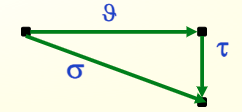
\includegraphics[width=\linewidth]{Assets/Logik_allgemeinster-unifikator.png}
  }

  Der Algorithmus zur Berechnung des m.g.u. zweier Terme $s$ und $t$ verwendet Unterscheidungsterme: Man lese $s$ und $t$ zeichenweise simultan von links nach rechts. Am ersten Zeichen, bei welchem sich $s$ und $t$ unterscheiden, beginnen die Unterscheidungsterme $s*$ und $t*$ und umfassen die dort beginnenden (vollständigen) Teilterme.

  Algorithmus zur Bestimmung des allgemeinsten Unifikators 2er Terme

  \begin{lstlisting}
  input: s, t
  output: Unifizierbarkeitsaussage, ggf. $\nu= m.g.u.( s , t )$
  $i:=0;\nu_i:=\varnothing;s_i:=s; t_i=t$
  Start: $s_i$ und $t_i$ identisch?
    ja $\Rightarrow$ s und t sind unifizierbar, $\nu=\nu_i=m.g.u.(s,t)$ (fertig)
    nein $\Rightarrow$ Bilde die Unterscheidungsterme $s_i^*$ und $t_i^*$
      $s_i^*$ oder $t_i^*$ Variable?
        nein $\Rightarrow$ $s$ und $t$ sind nicht unifizierbar (fertig)
        ja $\Rightarrow$ sei (o.B.d.A.) $s_i^*$ eine Variable
          $s_i^* \subseteq t_i^*$? (enthaelt $t_i^*$ die Variable $s_i^*$?)
            ja $\Rightarrow$ $s$ und $t$ sind nicht unifizierbar (fertig)
            nein $\Rightarrow$ 
              $\nu':=\{[s,t']: [s,t]\in\nu, t':=t|_{s*\rightarrow t*}\}\cup \{[s_i^*, t_i^*]\}$
              $s':=\nu'(s_i); t':=\nu'(t_i); i:=i+1;$
              $\nu_i:=\nu'; s_i:=s'; t_i:=t';$ 
              gehe zu Start
  \end{lstlisting}

  \subsection{Logische Programmierung}
  \subsubsection{Einordnung des logischen Paradigmas}
  %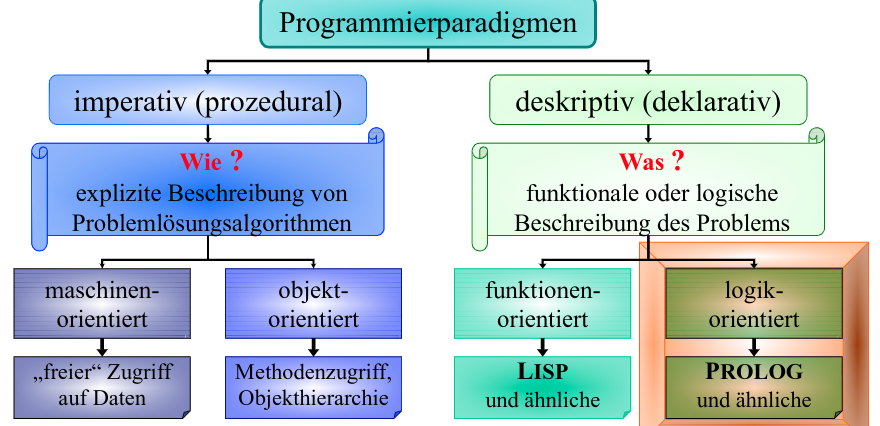
\includegraphics[width=\linewidth]{Assets/Logik-logische-programmierung-einordnung.png}

  "deskriptives" Programmierparadigma =
  \begin{enumerate*}
    \item Problembeschreibung
    \begin{itemize*}
      \item Die Aussagenmenge $M =\{K_1,...,K_n\}$, über denen gefolgert wird, wird in Form von Fakten und Regeln im PK1 notiert.
      \item Eine mutmaßliche Folgerung (Hypothese) $H$ wird in Form einer Frage als negierte Hypothese hinzugefügt.
    \end{itemize*}
    \item (+) Programmverarbeitung
    \begin{itemize*}
      \item Auf der Suche eines Beweises für $M \Vdash H$ werden durch mustergesteuerte Prozedur-Aufrufe Resolutions-Schritte zusammengestellt.
      \item Dem "Programmierer" werden (begrenzte) Möglichkeiten gegeben, die systematische Suche zu beeinflussen.
    \end{itemize*}
  \end{enumerate*}

  \subsubsection{Syntax}
  Syntax von Klauseln
  |       | Syntax                                                                                                     | Beispiel                                                                |
  | ----- | ---------------------------------------------------------------------------------------------------------- | ----------------------------------------------------------------------- |
  | Fakt  | praedikatensymbol(term,...term).                                                                           | $liefert(xy\_ag,motor,vw)$.                                                |
  | Regel | praedikatensymbol(term,...term) :- praedikatensymbol(term,...term) ,... , praedikatensymbol(term,...term). | konkurrenten(Fa1,Fa2) :- liefert(Fa1,Produkt,\_),liefert(Fa2,Produkt,\_). |
  | Frage | ?- praedikatensymbol(term,...term) , ... ,praedikatensymbol(term,...term).                                 | ?- konkurrenten(ibm,X), liefert(ibm,\_,X).                               |

  Syntax von Termen
  |                     |                                                                           | Syntax                                                                                      | Beispiele             |
  | ------------------- | ------------------------------------------------------------------------- | ------------------------------------------------------------------------------------------- | --------------------- |
  | Konstante           | Name                                                                      | Zeichenfolge, beginnend mit Kleinbuchstaben, die Buchstaben, Ziffern und \_ enthalten kann. | otto\_1 , tisch, hund |
  |                     | beliebige Zeichenfolge in "..." geschlossen                               | "Otto", "r@ho"                                                                              |
  |                     | Sonderzeichenfolge                                                        | €\%\&§\$€                                                                                      |
  | Zahl                | Ziffernfolge, ggf. mit Vorzeichen, Dezimalpunkt und Exponentendarstellung | 3, -5, 1001, 3.14E-12                                                                       |
  | Variable            | allg.                                                                     | Zeichenfolge, mit Großbuchstaben oder $\_$ beginnend                                          | X, Was, \_alter        |
  | anonym              | Unterstrich                                                               | \_                                                                                          |
  | strukturierter Term | allg.                                                                     | funktionssymbol( term , ... , term )                                                        | nachbar(chef(X))      |
  | Liste               | leere Liste                                                               | [ ]                                                                                         |
  |                     | $[term | restliste]$                                                                                 | $[mueller | [mayer | []]]$ |
  |                     | $[term , term , ... , term ]$                                             | $[ mueller, mayer, schulze ]$                                                               |

  BACKUS-NAUR-Form
  \begin{itemize*}
    \item PROLOG-Programm ::= Wissensbasis Hypothese
    \item Wissensbasis ::= Klausel | Klausel Wissensbasis
    \item Klausel ::= Fakt | Regel
    \item Fakt ::= Atomformel.
    \item Atomformel ::= Prädikatensymbol (Termfolge)
    \item Prädikatensymbol ::= Name
    \item Name ::= Kleinbuchstabe |Kleinbuchstabe Restname | "Zeichenfolge" | Sonderzeichenfolge
    \item RestName ::= Kleinbuchstabe | Ziffer | $\_$ | Kleinbuchstabe RestName | Ziffer RestName | \_ RestName
    \item ...
  \end{itemize*}

  \subsubsection{PROLOG aus logischer Sicht}
  Was muss der Programmierer tun?
  \begin{itemize*}
    \item Formulierung einer Menge von Fakten und Regeln (kurz: Klauseln), d.h. einer Wissensbasis $M\equiv\{K_1,...,K_n\}$
    \item Formulierung einer negierten Hypothese (Frage, Ziel) $\lnot H\equiv\bigwedge_{i=1}^m H_i \equiv false\leftarrow \bigwedge_{i=1}^m H_i$
  \end{itemize*}

  Was darf der Programmierer erwarten?
  \begin{itemize*}
    \item Dass das "Deduktionstool" PROLOG $M \Vdash H$ zu zeigen versucht, d.h. $kt(\bigwedge_{i=1}^n K_i\wedge \lnot H)$ )
    \item ..., indem systematisch die Resolutionsmethode auf $\lnot H$ und eine der Klauseln aus $M$ angewandt wird, solange bis $\lnot H\equiv false\leftarrow true$ entsteht
  \end{itemize*}

  \paragraph{Formulierung von Wissensbasen}
  Beispiel 1 (BSP1.PRO)
  \begin{itemize*}
    \item Yoshihito und Sadako sind die Eltern von Hirohito.
    \begin{itemize*}
      \item vater\_von(yoshihito,hirohito).
      \item mutter\_von(sadako,hirohito).
    \end{itemize*}
    \item Kuniyoshi und Chikako sind die Eltern von Nagako.
    \begin{itemize*}
      \item vater\_von(kunioshi,nagako).
      \item mutter\_von(chikako,nagako).
    \end{itemize*}
    \item Akihito‘s und Hitachi‘s Eltern sind Hirohito und Nagako.
    \begin{itemize*}
      \item vater\_von(hirohito,akihito).
      \item vater\_von(hirohito,hitachi).
      \item mutter\_von(nagako,akihito).
      \item mutter\_von(nagako,hitachi).
    \end{itemize*}
    \item Der Großvater ist der Vater des Vaters oder der Vater der Mutter.
    \begin{itemize*}
      \item grossvater\_von(G,E) :- vater\_von(G,V), vater\_von(V,E).
      \item grossvater\_von(G,E) :-vater\_von(G,M),mutter\_von(M,E).
    \end{itemize*}
    \item Geschwister haben den gleichen Vater und die gleiche Mutter.
    \begin{itemize*}
      \item geschwister(X,Y) :- vater\_von(V,X), vater\_von(V,Y), mutter\_von(M,X), mutter\_von(M,Y).
    \end{itemize*}
  \end{itemize*}

  Visual Prolog benötigt aber einen Deklarationsteil für Datentypen und Aritäten der Prädikate, der für die o.g. Wissensbasis so aussieht:
  \begin{lstlisting}
  domains
    person = symbol
  predicates
    vater_von(person,person)        % bei nichtdeterministischen Praedikaten
    mutter_von(person,person).      % kann man "nondeterm" vor das
    grossvater_von(person,person)   % Praedikat schreiben, um die
    geschwister(person,person)      % Kompilation effizienter zu machen
  clauses
    < Wissensbasis einfuegen und Klauseln gleichen Kopfpraedikates gruppieren>
  goal
    < Frage ohne "?-" einfuegen>
  \end{lstlisting}

  Deklarationsteil
  \begin{lstlisting}
  domains
    person, raum: symbol
  predicates
    arbeitet_in(person,raum)
    ansluss_in(raum)
    erreichbar(person)
    koennen_daten_austauschen(person,person)
  clauses
    ...
  goal
    ...
  \end{lstlisting}

  \paragraph{Verarbeitung Logischer Programme}
  \paragraph{Veranschaulichung ohne Unifikation}
  %\includegraphics[width=\linewidth]{Assets/Logik-prolog-ohne-unifikation.png)

  Tiefensuche mit Backtrack:
  Es werden anwendbare Klauseln für das erste Teilziel gesucht. Gibt es ...
  \begin{itemize*}
    \item ... genau eine, so wird das 1. Teilziel durch deren Körper ersetzt.
    \item ... mehrere, so wird das aktuelle Ziel inklusive alternativ anwendbarer Klauseln im Backtrack-Keller abgelegt und die am weitesten oben stehende Klausel angewandt.
    \item ... keine (mehr), so wird mit dem auf dem Backtrack-Keller liegendem Ziel die Bearbeitung fortgesetzt.
  \end{itemize*}

  Dies geschieht solange, bis
  \begin{itemize*}
    \item das aktuelle Ziel leer ist oder
    \item keine Klausel (mehr) anwendbar ist und der Backtrack-Keller leer ist.
  \end{itemize*}


  \paragraph{Veranschaulichung mit Unifikation}
  %\includegraphics[width=\linewidth]{Assets/Logik-prolog-mit-unifikation.png)

  Zusätzliche Markierung der Kanten mit der Variablenersetzung (dem Unifikator).


  \subsubsection{PROLOG aus prozeduraler Sicht}
  Beispiel: die "Hackordnung"
  \begin{enumerate*}
    \item chef\_von(mueller,mayer).
    \item chef\_von(mayer,otto).
    \item chef\_von(otto,walter).
    \item chef\_von(walter,schulze).
    \item weisungsrecht(X,Y) :- chef\_von(X,Y).
    \item weisungsrecht(X,Y) :- chef\_von(X,Z), weisungsrecht(Z,Y).
  \end{enumerate*}

  \note{Deklarative Interpretation}{In einem Objektbereich $I=\{mueller, mayer, schulze, ...\}$ bildet das Prädikat $weisungsrecht(X,Y)$ $[X,Y]$ auf wahr ab, gdw.
    \begin{itemize*}
      \item das Prädikat $chef_von(X,Y)$ das Paar $[X,Y]$ auf wahr abbildet oder
      \item es ein $Z\in I$ gibt, so dass
      \begin{itemize*}
        \item das Prädikat $chef_von(X,Z)$ das Paar $[X,Z]$ auf wahr abbildet und
        \item das Prädikat $weisungsrecht(Z,Y)$ das Paar $[Z,Y]$ auf wahr abbildet.
      \end{itemize*}
    \end{itemize*}
  }

  \note{Prozedurale Interpretation}{Die Prozedur $weisungsrecht(X,Y)$ wird abgearbeitet, indem
    \begin{enumerate*}
      \item die Unterprozedur $chef_von(X,Y)$ abgearbeitet wird. Im Erfolgsfall ist die Abarbeitung beendet; anderenfalls werden
      \item die Unterprozeduren $chef_von(X,Z)$ und $weisungsrecht(Z,Y)$ abgearbeitet; indem systematisch Prozedurvarianten beider Unterprozeduren aufgerufen werden. Dies geschieht bis zum Erfolgsfall oder erfolgloser erschöpfender Suche.
    \end{enumerate*}
  }


  | deklarative Interpretation         | prozedurale Interpretation |
  | ---------------------------------- | -------------------------- |
  | Prädikat                           | Prozedur                   |
  | Ziel                               | Prozeduraufruf             |
  | Teilziel                           | Unterprozedur              |
  | Klauseln mit gleichem Kopfprädikat | Prozedur-varianten         |
  | Klauselkopf                        | Prozedurkopf               |
  | Klauselkörper                      | Prozedurrumpf              |

  Die Gratwanderung zwischen Wünschenswertem und technisch Machbarem erfordert mitunter "Prozedurales Mitdenken", um
  \begin{enumerate*}
    \item eine gewünschte Reihenfolge konstruktiver Lösungen zu erzwingen,
    \item nicht terminierende (aber - deklarativ, d.h. logisch interpretiert - völlig korrekte) Programme zu vermeiden,
    \item seiteneffektbehaftete Prädikate sinnvoll einzusetzen,
    \item (laufzeit-) effizienter zu programmieren und
    \item das Suchverfahren gezielt zu manipulieren.
  \end{enumerate*}

  Programm inkl. Deklarationsteil (BSP3.PRO)
  \begin{lstlisting}
  domains
    person = symbol
  predicates
    chef_von(person,person)
    weisungsrecht(person,person)
  clauses
    chef_von(mueller,mayer).
    chef_von(mayer,otto).
    chef_von(otto,walter).
    chef_von(walter,schulze).
    weisungsrecht(X,Y) :- chef_von(X,Y).
    weisungsrecht(X,Y) :- chef_von(X,Z), weisungsrecht(Z,Y).
  goal
    weisungsrecht(Wer,Wem).
  \end{lstlisting}

  Prädikate zur Steuerung der Suche nach einer Folge von Resolutionsschritten!

  !(cut)
  Das Prädikat $!/0$ ist stets wahr. In Klauselkörpern eingefügt verhindert es ein Backtrack der hinter $!/0$ stehenden Teilziele zu den vor $!/0$ stehenden Teilzielen sowie zu alternativen Klauseln des gleichen Kopfprädikats. Die Verarbeitung von $!/0$ schneidet demnach alle vor der Verarbeitung verbliebenen Lösungswege betreffenden Prozedur ab.

  Prädikate zur Steuerung der Suche: $!/0$
  %\includegraphics[width=\linewidth]{Assets/Logik-prädikate-suche.png)


  Prädikate zur Steuerung der Suche nach einer Folge von Resolutionsschritten
  **fail**
  Das Prädikat $fail/0$ ist stets falsch. In Klauselkörpern eingefügt löst es ein Backtrack aus bzw. führt zum Misserfolg, falls der Backtrack-Keller leer ist, d.h. falls es keine verbleibenden Lösungswege (mehr) gibt.
  ![BSP4.PRO](Assets/Logik-prädikate-suche-fail.png)
  ![BSP4.PRO](Assets/Logik-prädikate-suche-fail-2.png)

  \subsubsection{Listen und rekursive Problemlösungsstrategien}
  Listen
  \begin{enumerate*}
    \item $[]$ ist eine Liste.
    \item Wenn $T$ ein Term und $L$ eine Liste ist, dann ist
    \begin{enumerate*}
      \item $[T|L]$ eine Liste.
      \item $T.L$ eine Liste. (ungebräuchlich)
      \item $.(T,L)$ eine Liste. (ungebräuchlich)
      \item Das erste Element $T$ heißt Listenkopf, $L$ heißt Listenkörper oder Restliste.
    \end{enumerate*}
    \item Wenn $t_1, ... ,t_n$ Terme sind, so ist $[t_1,...,t_n]$ eine Liste.
    \item Weitere Notationsformen von Listen gibt es nicht.
  \end{enumerate*}

  Listen als kompakte Wissensrepräsentation: ein bekanntes Beispiel (BSP5.PRO)
  \begin{lstlisting}
  - arbeiten_in([meier, mueller], raum_1).
    - arbeitet_in(meier, raum_1).
    - arbeitet_in(mueller, raum_1).
  - arbeitet_in(otto, raum_2).
    - arbeiten_in([otto], raum_2 ).
  - arbeitet_in(kraus, raum_3).
    - arbeiten_in([kraus], raum_3 ).
  - anschluesse_in([raum_2, raum_3]).
    - anschluss_in(raum_2).
    - anschluss_in(raum_3).
  \end{lstlisting}

  **Rekursion** in der Logischen Programmierung
  Eine Prozedur heißt (direkt) rekursiv, wenn in mindestens einem der Klauselkörper ihrer Klauseln ein erneuter Aufruf des Kopfprädikates erfolgt.
  Ist der Selbstaufruf die letzte Atomformel des Klauselkörpers der letzten Klausel dieser Prozedur - bzw. wird er es durch vorheriges "Abschneiden" nachfolgender
  Klauseln mit dem Prädikat $!/0$ - , so spricht man von Rechtsrekursion ; anderenfalls von Linksrekursion.
  Eine Prozedur heißt indirekt rekursiv, wenn bei der Abarbeitung ihres Aufrufes ein erneuter Aufruf derselben Prozedur erfolgt.

  Wissensverarbeitung mit Listen: (BSP5.PRO)
  \begin{lstlisting}
  - erreichbar(K) :- arbeitet_in(K,R), anschluss_in(R).
    - erreichbar(K) :- anschluesse_in(Rs), member(R, Rs), arbeiten_in(Ks, R), member(K, Ks).
  - koennen_daten_austauschen(K1,K2) :- arbeitet_in(K1,R),arbeitet_in(K2,R).
    - koennen_daten_austauschen(K1,K2) :- arbeiten_in(Ks,_),member(K1,Ks), member(K2,Ks).
  - koennen_daten_austauschen(K1,K2) :- erreichbar(K1),erreichbar(K2).
    - koennen_daten_austauschen(K1,K2) :- erreichbar(K1),erreichbar(K2).
  \end{lstlisting}

  BSP5.PRO
  \begin{lstlisting}
  domains
    person, raum = symbol
    raeume = raum*
    personen = person*
  predicates
    arbeiten_in(personen, raum)
    anschluesse_in(raeume)
    erreichbar(person)
    koennen_daten_austauschen(person,person)
    member(person,personen)
    member(raum,raeume)
  clauses
    ... (siehe oben)
    member(E,[E|_]).
    member(E,[_|R]) :- member(E,R).
  goal
    erreichbar(Wer).
  \end{lstlisting}

  **Unifikation 2er Listen**
  \begin{enumerate*}
    \item Zwei leere Listen sind (als identische Konstanten aufzufassen und daher) miteinander unifizierbar.
    \item Zwei nichtleere Listen $[K_1|R_1]$ und $[K_2|R_2]$ sind miteinander unifizierbar, wenn ihre Köpfe ($K_1$ und $K_2$) und ihre Restlisten ($R_1$ und $R_2$) jeweils miteinander unifizierbar sind.
    \item Eine Liste $L$ und eine Variable $X$ sind miteinander unifizierbar, wenn die Variable selbst nicht in der Liste enthalten ist. Die Variable $X$ wird bei erfolgreicher Unifikation mit der Liste $L$ instanziert: $X:=L$.
  \end{enumerate*}

  **Differenzlisten:** eine intuitive Erklärung
  Eine Differenzliste $L_1 - L_2$ besteht aus zwei Listen $L_1$ und $L_2$ und wird im allgemeinen als $[L_1,L_2]$ oder (bei vorheriger Definition eines pre- bzw. infix notierten Funktionssymbols
  -/2) als $-(L_1,L_2)$ bzw. $L_1-L_2$ notiert.

  Sie wird (vom Programmierer, nicht vom PROLOG-System!) als eine Liste interpretiert, deren Elemente sich aus denen von $L_1$ abzüglich derer von $L_2$ ergeben. Differenzlisten verwendet man typischerweise, wenn häufig Operationen am Ende von Listen vorzunehmen sind.

  Eine Definition
  \begin{enumerate*}
    \item Die Differenz aus einer leeren Liste und einer (beliebigen) Liste ist die leere Liste: $[] - L = []$
    \item Die Differenz aus einer Liste $[E|R]$ und der Liste $L$, welche $E$ enthält, ist die Liste $D$,
    wenn die Differenz aus $R$ und $L$ (abzügl. $E$) die Liste $D$ ist: $[E|R]-L = D$, wenn $E\in L$ und $R-(L-[E]) = D$
    \item Die Differenz aus einer Liste $[E|R]$ und einer Liste $L$, welche $E$ nicht enthält, ist die Liste $[E|D]$, wenn die Differenz aus $R$ und $L$ die Liste $D$ ist: $[E|R] - L = [E|D]$, wenn $E\in L$ und $R-L=D$
  \end{enumerate*}

  Differenzlisten: Ein Interpreter $interpret(Differenzliste,Interpretation)$ (BSP6.PRO)
  \begin{enumerate*}
    \item $interpret([[],_],[]).$
    \item $interpret([[E|R],L] , D ) :- loesche(E , L, L1),! , interpret( [ R , L1 ] , D ).$
    \item $interpret([[E|R],L] , [E|D] ) :- interpret([R,L],D).$
    \item $loesche(E, [E|R], R) :-!.$
    \item $loesche(E, [K|R], [K|L]) :- loesche(E,R,L).$
  \end{enumerate*}

  \subsubsection{Prolog-Fallen}
  \paragraph{Nicht terminierende Programme }
  Ursache: "ungeschickt" formulierte (direkte oder indirekte) Rekursion

  \paragraph{Alternierende Zielklauseln}
  Ein aktuelles Ziel wiederholt sich und die Suche nach einer Folge von Resolutionsschritten endet nie:
  \begin{enumerate*}
    \item $liegt_auf(X,Y) :- liegt_unter(Y,X).$
    \item $liegt_unter(X,Y) :- liegt_auf(Y,X).$
  \end{enumerate*}
  \begin{itemize*}
    \item $?- liegt_auf( skript, pult ).$
    \item logisch korrekte Antwort: nein
    \item tatsächliche Antwort: keine
  \end{itemize*}

  oder die Suche nach Resolutionsschritten endet mit einem Überlauf des Backtrack-Kellers: (BSP8.PRO)
  \begin{enumerate*}
    \item $liegt_auf(X,Y) :- liegt_unter(Y,X).$
    \item $liegt_auf( skript , pult ).$
    \item $liegt_unter(X,Y) :- liegt_auf(Y,X).$
  \end{enumerate*}
  \begin{itemize*}
    \item $?- liegt_auf( skript , pult ).$
    \item logisch korrekte Antwort: ja
    \item tatsächliche Antwort: keine
  \end{itemize*}

  \paragraph{Expandierende Zielklauseln }
  Das erste Teilziel wird in jeden Resolutionsschritt durch mehrere neue Teilziele ersetzt; die Suche endet mit einem Speicherüberlauf: (BSP9.PRO)
  \begin{enumerate*}
    \item $liegt_auf( notebook , pult ).$
    \item $liegt_auf( skript , notebook ).$
    \item $liegt_auf(X,Y) :- liegt_auf(X,Z), liegt_auf(Z,Y).$
  \end{enumerate*}
  \begin{itemize*}
    \item $?- liegt_auf( handy , skript ).$
    \item logisch korrekte Antwort: nein
    \item tatsächliche Antwort: keine
  \end{itemize*}

  Auch dieses Beispiel lässt sich so erweitern, dass die Hypothese offensichtlich aus der Wissensbasis folgt, die Umsetzung der Resolutionsmethode aber die Vollständigkeit zerstört:
  \begin{enumerate*}
    \item $liegt_auf( notebook , pult ).$
    \item $liegt_auf( skript , notebook ).$
    \item $liegt_auf(X,Y) :- liegt_auf(X,Z), liegt_auf(Z,Y).$
    \item $liegt_auf( handy , skript ).$
  \end{enumerate*}
  \begin{itemize*}
    \item $?- liegt_auf( handy , pult ).$
    \item logisch korrekte Antwort: ja
    \item tatsächliche Antwort: keine
  \end{itemize*}

  Auch dieses Beispiel zeigt, dass das Suchverfahren "Tiefensuche mit Backtrack" die Vollständigkeit des Inferenzverfahrens zerstört.

  \paragraph{Metalogische Prädikate und konstruktive Lösungen}
  Das Prädikat $not/1$ hat eine Aussage als Argument und ist somit eine Aussage über eine Aussage, also metalogisch.
  I.allg. ist $not/1$ vordefiniert, kann aber mit Hilfe von $call/1$ definiert werden. $call/1$ hat Erfolg, wenn sein Argument - als Ziel interpretiert - Erfolg hat.

  Beispiel (BSP10.PRO):
  \begin{enumerate*}
    \item $fleissig(horst).$
    \item $fleissig(martin).$
    \item $faul(X) :- not( fleissig(X) ).$
    \item $not(X) :- call(X), !, fail.$
    \item $not( _ ).$
  \end{enumerate*}
  \begin{itemize*}
    \item $?- faul(horst).$ Antwort: nein
    \item $?- faul(alex).$ Antwort: ja
    \item $?- faul(Wer).$ Antwort: nein
  \end{itemize*}

  Widerspruch ... und Beweis der Unvollständigkeit durch Metalogik

  \subsubsection{Typische Problemklassen für die Anwendung der Logischen Programmierung}
  \paragraph{Rekursive Problemlösungsstrategien}
  \note{Botschaft  1}{Man muss ein Problem nicht in allen Ebenen überblicken, um eine Lösungsverfahren zu programmieren. Es genügt die Einsicht,
    \begin{enumerate*}
      \item wie man aus der Lösung eines einfacheren Problems die Lösung des präsenten Problems macht und
      \item wie es im Trivialfall zu lösen ist.
    \end{enumerate*}
  }

  **Türme von Hanoi**
  Es sind N Scheiben von der linken Säule auf die mittlere Säule zu transportieren, wobei die rechte Säule als Zwischenablage genutzt wird. Regeln:
  \begin{enumerate*}
    \item Es darf jeweils nur eine Scheibe transportiert werden.
    \item Die Scheiben müssen mit fallendem Durchmesser übereinander abgelegt werden.
  \end{enumerate*}

  (doppelt) rekursive Lösungsstrategie:
  \begin{itemize*}
    \item $N = 0:$ Das Problem ist gelöst.
    \item $N > 0:$
    \begin{enumerate*}
      \item Man löse das Problem für N-Scheiben, die von der Start-Säule zur Hilfs-Säule zu transportieren sind.
      \item Man lege eine Scheibe von der Start- zur Ziel-Säule.
      \item Man löse das Problem für N-Scheiben, die von der Hilfs-Säule zur Ziel-Säule zu transportieren sind.
    \end{enumerate*}
  \end{itemize*}

  Prädikate
  \begin{itemize*}
    \item $hanoi(N)$ löst das Problem für N Scheiben
    \item $verlege(N,Start,Ziel,Hilf)$ verlegt N Scheiben von Start nach Ziel unter Nutzung von Hilf als Ablage
  \end{itemize*}

  Die Regeln zur Kodierung der Strategie (BSP11.PRO)
  \begin{itemize*}
    \item $hanoi( N ) :- verlege( N , s1 , s2 , s3 ).$
    \item $verlege( 0 , \_ , \_ , \_ ).$
    \item $verlege( N , S , Z , H ) :-$
    \begin{itemize*}
      \item $N1 = N - 1,$
      \item $verlege( N1 , S , H , Z ),$
      \item $write("Scheibe\ von ", S," nach ", Z),$
      \item $verlege( N1 , H , Z , S ).$
    \end{itemize*}
  \end{itemize*}

  \paragraph{Sprachverarbeitung mit PROLOG}
  \note{Botschaft  2}{Wann immer man Objekte mit Mustern vergleicht, z.B.
    \begin{enumerate*}
      \item eine Struktur durch "Auflegen von Schablonen" identifiziert,
      \item Gemeinsamkeiten mehrerer Objekte identifiziert, d.h. "eine Schablone entwirft" oder
      \item "gemeinsame Beispiele für mehrere Schablonen" sucht,
    \end{enumerate*}
    mache man sich den Unifikations-Mechanismus zu nutzen.}

  \begin{itemize*}
    \item Eine kontextfreie Grammatik (Chomsky-Typ 2) besteht aus
    \begin{enumerate*}
      \item einem Alphabet A, welches die terminalen (satzbildenden) Symbole enthält
      \item einer Menge nichtterminaler (satzbeschreibender) Symbole N (= Vokabular abzüglich des Alphabets: $N = V \backslash A$)
      \item einer Menge von Ableitungsregeln $R\subseteq N\times (N\cup A)^*$
      \item dem Satzsymbol $S\in N$
    \end{enumerate*}
    \item ... und in PROLOG repräsentiert werden durch
    \begin{enumerate*}
      \item 1-elementige Listen, welche zu satzbildenden Listen komponiert werden: $[der],[tisch],[liegt],...$
      \item Namen, d.h. mit kleinem Buchstaben beginnende Zeichenfolgen: $nebensatz,subjekt,attribut,...$
      \item PROLOG-Regeln mit $l\in N$ im Kopf und $r\in(N\cup A)^*$ im Körper
      \item einen reservierten Namen: $satz$
    \end{enumerate*}
  \end{itemize*}

  Ein Ableitungsbaum beschreibt die grammatische Struktur eines Satzes. Seine Wurzel ist das Satzsymbol, seine Blätter in Hauptreihenfolge bilden den Satz.
  %\includegraphics[width=\linewidth]{Assets/Logik-ableitungsbaum-beispiel.png)

  \begin{enumerate*}
    \item Alphabet $ministerium, rektorat, problem, das, loest, ignoriert, verschaerft$
    \item nichtterminale Symbole $satz, subjekt, substantiv, artikel, praedikat,objekt$
    \item Ableitungsregeln (in BACKUS-NAUR-Form)
  \end{enumerate*}
  \begin{itemize*}
    \item $satz ::= subjekt praedikat objekt$
    \item $subjekt ::= artikel substantiv$
    \item $objekt ::=  artikel substantiv$
    \item $substantiv ::= ministerium | rektorat | problem$
    \item $artikel ::= das$
    \item $praedikat ::= loest | ignoriert | verschaerft$
  \end{itemize*}
  4. Satzsymbol $satz$

  Verketten einer Liste von Listen
  ```
  % die Liste ist leer
  verkette( [ ] , [ ] ) .

  % das erste Element ist eine leere Liste
  verkette( [ [ ] | Rest ] , L ) :-
  verkette( Rest , L ).

  % das erste Element ist eine nichtleere Liste
  verkette([ [K | R ] | Rest ] , [ K | L ] ) :-
  verkette( [ R | Rest ] , L ).4
  ```

  \paragraph{Die "Generate - and - Test" Strategie}
  \note{Botschaft  3}{Es ist mitunter leichter (oder überhaupt erst möglich), für komplexe Probleme
    \begin{enumerate*}
      \item eine potentielle Lösung zu "erraten" und dazu
      \item ein Verfahren zu entwickeln, welches diese Lösung auf Korrektheit testet,
    \end{enumerate*}
    als zielgerichtet die korrekte Lösung zu entwerfen. Hierbei kann man den Backtrack-Mechanismus nutzen.}

  Strategie: Ein Prädikat $moegliche_loesung(L)$ generiert eine potentielle Lösung, welche von einem Prädikat $korrekte_loesung(L)$ geprüft wird:
  \begin{itemize*}
    \item Besteht $L$ diesen Korrektheitstest, ist eine Lösung gefunden.
    \item Fällt $L$ bei diesem Korrektheitstest durch, wird mit Backtrack das Prädikat $moegliche_loesung(L)$ um eine alternative potentielle Lösung ersucht.
    (vgl.: Lösen NP-vollständiger Probleme, Entscheidung von Erfüllbarkeit)
  \end{itemize*}

  ein Beispiel: konfliktfreie Anordnung von $N$ Damen auf einem $N\times N$ Schachbrett (BSP13.PRO)
  \begin{itemize*}
    \item eine Variante: Liste strukturierter Terme
    \begin{itemize*}
      \item $[dame(Zeile,Spalte),...,dame(Zeile,Spalte)]$
      \item $[dame(1,2), dame(2,4), dame(3,1), dame(4,3) ]$
    \end{itemize*}
    \item noch eine Variante: Liste von Listen
    \begin{itemize*}
      \item $[[Zeile, Spalte] , ... , [Zeile,Spalte] ]$
      \item $[ [1,2] , [2,4] , [3,1] , [4,3] ]$
    \end{itemize*}
    \item ... und noch eine (in die Wissensdarstellung etwas "natürliche" Intelligenz investierende, den Problemraum enorm einschränkende) Variante: Liste der Spaltenindizes
    \begin{itemize*}
      \item $[ Spalte_zu_Zeile_1, ..., Spalte_zu_Zeile_N ]$
      \item $[ 2, 4, 1, 3 ]$
    \end{itemize*}
  \end{itemize*}

  \paragraph{Heuristische Problemlösungsmethoden}
  \note{Botschaft  4}{Heuristiken sind
    \begin{enumerate*}
      \item eine Chance, auch solche Probleme einer Lösung zuzuführen, für die man keinen (determinierten) Lösungsalgorithmus kennt und
      \item das klassische Einsatzgebiet zahlreicher KI-Tools - auch der Logischen Programmierung.
    \end{enumerate*}
  }

  Was ist eine Heuristik? Worin unterscheidet sich eine heuristische Problemlösungsmethode von einem Lösungsalgorithmus?

  Heuristiken bewerten die Erfolgsaussichten alternativer Problemlösungsschritte. Eine solche Bewertung kann sich z.B. ausdrücken in
  \begin{itemize*}
    \item einer quantitativen Abschätzung der "Entfernung" zum gewünschten Ziel oder der "Kosten" für das Erreichen des Ziels,
    \item einer quantitativen Abschätzung des Nutzens und/oder der Kosten der alternativen nächsten Schritte,
    \item eine Vorschrift zur Rangordnung der Anwendung alternativer Schritte, z.B. durch Prioritäten oder gemäß einer sequenziell abzuarbeitenden Checkliste.
  \end{itemize*}

  Ein Beispiel: Das Milchgeschäft meiner Großeltern in den 40er Jahren
  \begin{itemize*}
    \item Der Milchhof liefert Milch in großen Kannen.
    \item Kunden können Milch nur in kleinen Mengen kaufen.
    \item Es gibt nur 2 Sorten geeichter Schöpfgefäße; sie fassen 0.75 Liter bzw. 1.25 Liter.
    \item Eine Kundin wünscht einen Liter Milch.
  \end{itemize*}
  \begin{enumerate*}
    \item Wenn das große Gefäß leer ist, dann fülle es.
    \item Wenn das kleine Gefäß voll ist, dann leere es.
    \item Wenn beides nicht zutrifft, dann schütte so viel wie möglich vom großen in das kleine Gefäß.
  \end{enumerate*}

  Prädikat $miss_ab(VolGr, VolKl, Ziel, InhGr, InhKl)$ mit
  \begin{itemize*}
    \item VolGr -  Volumen des großen Gefäßes
    \item VolKl -  Volumen des kleinen Gefäßes
    \item Ziel - die abzumessende (Ziel-) Menge
    \item InhGr - der aktuelle Inhalt im großen Gefäß
    \item InhKl - der aktuelle Inhalt im kleinen Gefäß
  \end{itemize*}

  Beispiel-Problem: $?- miss_ab( 1.25 , 0.75 , 1 , 0 , 0 )4$

  \paragraph{Pfadsuche in gerichteten Graphen}
  \note{Botschaft  5}{
    1. Für die systematische Suche eines Pfades kann der Suchprozess einer Folge von Resolutionsschritten genutzt werden. Man muss den Suchprozess nicht selbst programmieren.
    2. Für eine heuristische Suche eines Pfades gilt Botschaft 4: Sie ist das klassische Einsatzgebiet zahlreicher KI-Tools - auch der Logischen Programmierung.
  }

  Anwendungen
  \begin{itemize*}
    \item Handlungsplanung, z.B.
    \begin{itemize*}
      \item Suche einer Folge von Bearbeitungsschritten für ein Produkt, eine Dienstleistung, einen "Bürokratischen Vorgang"
      \item Suche eines optimalen Transportweges in einem Netzwerk von Straßen-, Bahn-, Flugverbindungen
    \end{itemize*}
    \item Programmsynthese = Handlungsplanung mit ...
    \begin{itemize*}
      \item ... Schnittstellen für die Datenübergabe zwischen "Handlungsschritten" (= Prozeduraufrufen) und
      \item ... einem hierarchischen Prozedurkonzept, welches die Konfigurierung von "Programmbausteinen" auf mehreren Hierarchie-Ebenen
    \end{itemize*}
  \end{itemize*}

  Ein Beispiel: Suche einer zeitoptimalen Flugverbindung (BSP15.PRO)
  \begin{itemize*}
    \item Repräsentation als Faktenbasis $verbindung(Start,Zeit1,Ziel,Zeit2,Tag).$
    \item Start -  Ort des Starts
    \item Zeit1 - Zeit des Starts
    \item Ziel - Ort der Landung
    \item Zeit2 - Zeit der Landung
    \item Tag - 0, falls Zeit1 und Zeit2 am gleichen Tag und 1 ansonsten
    \item möglich:
    \begin{itemize*}
      \item $verbindung(fra,z(11,45),ptb,z(21,0),0).$
      \item $verbindung(fra,z(11,15),atl,z(21,25),0).$
      \item $verbindung(ptb,z(24,0),orl,z(2,14),1).$
      \item $verbindung(atl,z(23,30),orl,z(0,54),1).$
    \end{itemize*}
  \end{itemize*}

  In einer dynamischen Wissensbasis wird die bislang günstigste Verbindung in Form eines Faktes $guenstigste([ v(Von,Zeit1,Nach,Zeit2,Tag), ... ], Ankunftszeit, Tag ).$ festgehalten und mit den eingebauten Prädikaten $assert(<Fakt>)$ - zum Einfügen des Faktes - und $retract (<Fakt>)$ - zum Entfernen des Faktes - bei Bedarf aktualisiert.
  Zum Beispiel $guenstigste([v(fra,z(11,45),ptb,z(21,00),0),v(ptb,z(24,0),orl,z(2,14),1)],z(2,14),1).$ erklärt den Weg über Pittsburgh zum bislang günstigsten gefundenen Weg.

  \paragraph{"Logeleien" als Prolog-Wissensbasen}
  \note{Botschaft 6}{
    \begin{enumerate*}
      \item "Logeleien" sind oft Aussagen über Belegungen von Variablen mit endlichem Wertebereich, ergänzt um eine Frage zu einem nicht explizit gegebenen Wert.
      \item Dabei handelt es sich um Grunde um eine Deduktionsaufgabe mit einer Hypothese zu einem mutmaßlichen Wert der gesuchten Variablen. Deshalb ist es oft auch mit dem "Deduktionstool" Prolog lösbar, denn Prolog tut im Grunde nichts anderes als ein ziel-gerichtetes "Durchprobieren" legitimer Deduktionsschritte im "Generate - and - Test" - Verfahren.
    \end{enumerate*}
  }


  Beispiel SUDOKU (BSP17.PRO)

  \paragraph{Tools für die formale Logik}
  \note{Botschaft 7}{Auch in der formalen Logik gibt es Deduktionsaufgaben, bei der Variablenbelegungen gesucht sind, welche eine Aussage wahr machen:
    \begin{enumerate*}
      \item Meist geschieht das durch systematische Auswertung der Aussage, wozu das Suchverfahren von Prolog genutzt werden kann.
      \item Auch hier geht es oft um gesuchte Werte für Variablen. Deshalb ist es oft auch mit dem "Deduktionstool" Prolog lösbar, denn Prolog tut im Grunde nichts anderes als ein ziel-gerichtetes "Durchprobieren" legitimer Deduktionsschritte im "Generate - and - Test" - Verfahren.
    \end{enumerate*}
  }

  Repräsentation von Aussagen als PROLOG-Term:
  \begin{itemize*}
    \item true, false: atom(true), atom(false)
    \item $A1\wedge A2$: und(A1,A2)
    \item $A1\vee A2$: oder(A1,A2)
    \item $\lnot A$: nicht(A)
    \item $A1\rightarrow A2$: wenndann(A1,A2)
    \item $A1\leftarrow A2$: dannwenn(A1,A2)
    \item $A1\leftrightarrow A2$: gdw(A1,A2)
  \end{itemize*}

  Erfüllbarkeitstest:
  \begin{itemize*}
    \item $?- erfuellbar(gdw(wenndann(nicht(oder(atom(false),atom(X))),atom(Y)), atom(Z))).$
    \item X=true, Y=\_, Z=true ; steht für 2 Modelle (eines mit Y = true und eines mit Y = false)
    \item X=false, Y=true, Z=true
  \end{itemize*}

  Ketten von Konjunktionen und Disjunktionen als PROLOG-Listen:
  \begin{itemize*}
    \item $A1\wedge A2\wedge ... \wedge An$: und verkettung([A1,A2, ..., An])
    \item $A1\vee A2\vee ...\vee An$: oder verkettung([A1,A2, ..., An])
  \end{itemize*}

  Erfüllbarkeitstest:
  \begin{itemize*}
    \item $?- erfuellbar(undverkettung([true,X,Y,true]))$
    \item X = true, Y = true
    \item $?- erfuellbar(oderverkettung([false,X,Y,false]))$
    \item X = true, Y = \_
    \item X = \_, Y = true
  \end{itemize*}

  Repräsentation von Termen als PROLOG-Term:
  \begin{itemize*}
    \item Wert: atom(<reelle Zahl>)
    \item $A1\wedge A2$: und(A1,A2)
    \item $A1\vee A2$: oder(A1,A2)
    \item $\lnot A$: nicht(A)
    \item $A1\rightarrow A2$: wenndann(A1,A2)
    \item $A1\leftarrow A2$: dannwenn(A1,A2)
    \item $A1\leftrightarrow A2$: gdw(A1,A2)
    \item $A1\wedge A2\wedge ... \wedge An$: und verkettung([A1,A2, ..., An])
    \item $A1\vee A2\vee ...\vee An$: oder verkettung([A1,A2, ..., An])
  \end{itemize*}

  Termauswertung:
  \begin{itemize*}
    \item $?- hat_wert(und(atom(0.5),oder(atom(0.7),atom(0.3))),X).$
    \item X=0.5
  \end{itemize*}

  Termauswertung unter Vorgabe des Wertebereiches:
  \begin{itemize*}
    \item $?- hat_wert([0,0.3, 0.5, 0.7, 1], und(atom(X),oder(atom(0.5),atom(0.7))),Wert).$
    \item X=0, Wert=0
    \item X=0.3, Wert=0.3
    \item X=0.5, Wert=0.5
    \item X=0.7, Wert=0.7
    \item X=1, Wert=0.7
  \end{itemize*}

\end{multicols}
\end{document}